\documentclass{article}
\usepackage{graphicx} % Required for inserting images
\usepackage[T1]{fontenc}
\usepackage[polish]{babel}
\usepackage[utf8]{inputenc}
\usepackage[a4paper, total={6in, 8in}]{geometry}
\usepackage{hyperref}
\usepackage{csquotes}
\usepackage{flafter}
\usepackage{float}
\usepackage{pgfplots}
\usepackage{multirow}
\usepackage{colortbl}
\usepackage{xpatch}
\usepackage{xcolor}
\usepackage{realboxes}
\usepackage{cleveref}

\usepackage{listings}
\newcommand{\chapref}[1]{[p. Rozdział~\ref{#1}]}


%New colors defined below
\definecolor{mygray}{rgb}{0.8,0.8,0.8}
\lstset{
  basicstyle=\ttfamily,
  backgroundcolor=\color{mygray},
}
\makeatletter
\xpretocmd\lstinline{\Colorbox{mygray}\bgroup\appto\lst@DeInit{\egroup}}{}{}
\makeatother

\definecolor{codegreen}{rgb}{0,0.6,0}
\definecolor{codegray}{rgb}{0.5,0.5,0.5}
\definecolor{codepurple}{rgb}{0.58,0,0.82}
\definecolor{backcolour}{rgb}{0.95,0.95,0.92}

%Code listing style named "mystyle"
\lstdefinestyle{mystyle}{
  backgroundcolor=\color{backcolour},   commentstyle=\color{codegreen},
  keywordstyle=\color{magenta},
  numberstyle=\tiny\color{codegray},
  stringstyle=\color{codepurple},
  basicstyle=\ttfamily\footnotesize,
  breakatwhitespace=false,         
  breaklines=true,                 
  captionpos=b,                    
  keepspaces=true,                 
  numbers=left,                    
  numbersep=5pt,                  
  showspaces=false,                
  showstringspaces=false,
  showtabs=false,                  
  tabsize=2
}

%"mystyle" code listing set
\lstset{style=mystyle}

\title{Kultura DevOps i współczesne rozwiązania CI/CD}
\author{Aleksander Błaszkiewicz}
\date{Styczeń 2024}

\begin{document}

\maketitle
\newpage
\tableofcontents
\newpage

\section{Wstęp}
Kultura DevOps reprezentuje syntezę filozofii, praktyk oraz narzędzi, które są kluczowe w zwiększaniu zdolności organizacji do efektywnego dostarczania aplikacji i usług w akcelerowanym tempie. Ta koncepcja ewoluowała jako odpowiedź na rosnącą potrzebę lepszej komunikacji, współpracy i integracji między działami rozwoju oprogramowania (Dev) i operacjami IT (Ops).

Za rok, w którym narodziła się ta kultura uważa się rok 2009. To wtedy John Allspaw (starszy wiceprezes ds. operacji technicznych) oraz Paul Hammond (dyrektor inżynieryjny) wygłosili słynną prezentację "10+ Deploys per Day: Dev and Ops Cooperation at Flickr"\cite{flickr}. Z kolei za ojca tej kultury uważa się Patricka Deboisa - który zainspirowany prezentacją zorganizował własną konferencję o nazwie DevOpsDays, która popularna jest aż do dzisiaj.

Rozwój tej kultury, chociaż silnie związany z programowaniem, wydaje się być opóźniony w stosunku do ewolucji samego programowania. Kultura DevOps, będąc reakcją na dynamiczny rozwój branży programistycznej, dopiero niedawno wkroczyła w fazę ustalania i konsolidacji najlepszych praktyk, analogicznie do etapu, w którym programowanie zaczęło koncentrować się na koncepcjach takich jak "czysty kod".\cite{stateOfDevops}

Jeszcze dekadę temu, umiejętność autonomicznego wdrażania aplikacji była rzadkością, wymagającą dogłębnej wiedzy o narzędziach i zasadach działania systemów operacyjnych. Obecnie, implementacja automatycznego systemu wdrażania aplikacji wielośrodowiskowych na serwerze jest możliwa w znacznie krótszym czasie. Przypisuję to zjawisko rozwojowi narzędzi o wysokim stopniu abstrakcji, które nazwałbym "meta-narzędziami"\chapref{subsectionMetaNarzedzia}. Pod tym terminem rozumiem narzędzia wykorzystujące inne narzędzia do jeszcze bardziej efektywnego osiągania określonych celów. Warto zauważyć, że to nie koniec - istnieją "meta-meta-narzędzia", które integrują wiele "meta-narzędzi".

Obserwuje się trend, w którym końcowy użytkownik tych rozwiązań jest coraz bardziej oddalony od pierwotnego celu, który stara się osiągnąć, co skutkuje ograniczeniem jego potrzeby posiadania szczegółowej wiedzy na temat działania tych systemów. Ma to swoje zalety, jak ułatwienie osiągania celów, ale również wady, takie jak utrzymanie użytkownika w nieświadomości konsekwencji niektórych decyzji. \cite{devOpsHandbook}. Jednym z typowych przykładów jest nieoptymalne wykorzystanie zasobów chmurowych i rachunki sięgające setek tysięcy dolarów spowodowane niewłaściwą konfiguracją.

Tematem niniejszej pracy jest analiza oraz praktyczne wdrożenie elementów kultury DevOps w kontekście projektu aplikacji. Praca skupia się przede wszystkim na procesach i rozwiązaniach związanych z implementacją, automatyzacją oraz utrzymaniem wysokiej jakości systemów IT. 

Kluczowym celem jest ukazanie, jak różne narzędzia oraz strategie DevOps mogą zostać wykorzystane do stworzenia aplikacji charakteryzującej się wysokim poziomem bezpieczeństwa, wydajności, kontrolą nad zmianami oraz zdolnością do testowania nowych wersji w niezależnych środowiskach. Opracowanie obejmuje zarówno teoretyczne analizy, jak i praktyczne wskazówki dotyczące implementacji, dzięki czemu dostarcza kompleksowego obrazu procesu wdrażania kultury DevOps.

Poruszone zagadnienia obejmują analizę i porównanie różnych podejść oraz narzędzi w zakresie budowy, wdrażania, monitorowania i utrzymania aplikacji. Każdy z aspektów został szczegółowo omówiony, wskazując zarówno wyzwania, jak i optymalne rozwiązania w kontekście współczesnych wymagań technologicznych oraz praktyk DevOps.

\subsection{Cele pracy}

Celem niniejszej pracy było stworzenie aplikacji o architekturze frontendowej i backendowej oraz szczegółowe omówienie procesu wdrażania kultury DevOps w takim projekcie. Tego typu architektura została wybrana ze względu na jej reprezentatywność dla typowych projektów realizowanych w środowiskach korporacyjnych, gdzie aplikacje często mają złożoną warstwę logiki biznesowej (backend) oraz interfejs użytkownika dostępny z poziomu przeglądarki lub aplikacji mobilnej (frontend).

Główny nacisk położono nie na opis samej aplikacji, lecz na aspekty związane z kulturą DevOps. W efekcie aplikacja cechuje się wysokim poziomem bezpieczeństwa, szybkim procesem budowania, kontrolą nad wprowadzanymi zmianami oraz możliwością testowania nowych wersji w odrębnym środowisku. W przypadku wystąpienia problemów z serwerem lub aplikacją generowany jest alert informujący o nieprawidłowościach.

Poruszone zagadnienia obejmują:

\begin{itemize}
    \item porównanie strategii budowy obrazów i wdrażania aplikacji pod względem czasu, zajętości miejsca, bezpieczeństwa oraz doświadczenia deweloperów (developer experience), wybór optymalnej strategii i opis jej implementacji,
    \item zarządzanie sekretami — opis koncepcji przechowywania wrażliwych danych w platformach CI/CD oraz implementacja tego rozwiązania,
    \item wielośrodowiskowość — omówienie potrzeby istnienia kilku środowisk (np. testowe, produkcyjne) oraz opis ich implementacji,
    \item porównanie podejść do monitoringu i obserwowalności, wybór najlepszych rozwiązań i opis ich implementacji,
    \item analizę wpływu zastosowanego narzędzia budującego backend (Babel vs SWC) na wydajność i czas budowy aplikacji,
    \item analizę wpływu narzędzia budującego frontend (CRA oraz Vite) na wydajność procesu budowy oraz użytkowania aplikacji,
    \item porównanie platform CI/CD, uwzględniające ich zalety, wady oraz rekomendacje dotyczące wyboru rozwiązania dostosowanego do potrzeb projektu,
    \item porównanie strategii budowy oraz zarządzania reverse proxy, uwzględniając aspekty wydajności, bezpieczeństwa oraz łatwości integracji z aplikacją,
    \item porównanie strategii wdrażania aplikacji,
    \item kompleksowy opis sposobu zarządzania serwerem w kontekście wdrażania i utrzymania aplikacji,
    \item opracowanie wytycznych dotyczących pisania wydajnych i czytelnych pipeline’ów \chapref{pipeline} na platformie GitHub Actions.
    \item porównanie podejść i narzędzi służących do monitorowania serwera oraz stanu aplikacji.
\end{itemize}

\section {DevOps}

\subsection{Definicja}

Na początku warto przytoczyć porównanie zaproponowane przez Patricka Deboisa\cite{devOpsHandbook}.

\begin{displayquote}
    I've settled on my own definition of "DevOps": everything you do to overcome the friction between silos. All the rest is plain engineering.
\end{displayquote}

Mówi on o zjawisku pojawianiu się granic pomiędzy drużyną deweloperów a „opsów” (tj. zespołu odpowiedzialnego za operacje, utrzymanie i zarządzanie infrastrukturą IT). Zaznacza, że jest to niekorzystne dla procesu wytwarzania oprogramowania, jako że informacje nie są poprawnie propagowane między wszystkimi zainteresowanymi. Definiuje DevOps jako wszystko, co robi się, aby zatrzeć te granice. Reszte traktuję jako czystą inżynierię.
\newline

Bardzo podobnie definiuje to Damon Edwards\cite{damonEdwards}.

\begin{displayquote}
    DevOps is, in many ways, an umbrella concept that refers to anything that smoothes out the interaction between development and operations.
\end{displayquote}

Ja zdefiniowałbym DevOps jako zestaw praktyk dążących do tego, żeby wytwarzanie oprogramowania było jak najłatwiejszym, dobrze ustrukturyzowanym i samodokumentującym się procesem.


\subsection{Filary}
W ramach grupy DevOps można wyróżnić określone pozycje:
\begin{itemize}
    \item współpraca - podstawa zasada DevOps. Oznacza współpracę pomiędzy zespołami zajmującymi się rozwojem (Dev) i operacjami (Ops). Ta metodyka przekształca tradycyjne podejście, w którym wyraźnie oddzielone były role związane z tworzeniem oprogramowania od tych związanych z jego wdrażaniem i utrzymaniem, w kierunku modelu, gdzie zespoły współpracują na każdym etapie cyklu życia aplikacji,
    \item automatyzacja - maksymalne ograniczenie ręcznych interwencji, co pozwala deweloperom skupić się na bardziej istotnych zadaniach, takich jak pisanie kodu czy rozwijanie nowych funkcji. W kontekście DevOps, automatyzacja jest nieodłącznym elementem procesu CI/CD (Continuous Integration/Continuous Delivery), co przekłada się na redukcję ludzkich błędów oraz zwiększenie produktywności zespołów,
    \item ciągłe doskonalenie - praktyka skoncentrowana na eksperymentowaniu oraz optymalizacji pod kątem szybkości, kosztów i łatwości dostawy. Ciągłe doskonalenie ściśle wiąże się również z ciągłym dostarczaniem (continuous delivery), umożliwiając zespołom DevOps nieustanne wdrażanie aktualizacji, które zwiększają efektywność systemów oprogramowania,
    \item rozumienie potrzeb - zespoły nie powinny pracować w oderwaniu od rzeczywistości ("budować w bańce"), tworząc oprogramowanie bazując tylko na założeniach, w jaki sposób użytkownicy będą z niego korzystać. Zamiast tego, zespoły DevOps powinny posiadać całkowite zrozumienie produktu, począwsy od jego tworzenia, aż po wdrożenie.
\end{itemize}

\subsection{Dostępne narzędzia}

W niniejszym podrozdziale skategoryzowano dostępne narzędzia, które zostaną szczegółowo omówione w dalszej części pracy:

\begin{itemize}
    \item budowa aplikacji NodeJS \chapref{sectionBudowanieAplikacji} - webpack, vite, SWC,
    \item platformy CI/CD \chapref{sectionCICD} - Gitlab, Github Actions,
    \item konteneryzacja \chapref{sectionBudowaObrazu} - docker,
    \item monitorowanie i observability - uptime kuma, grafana, prometheus, loki, cadvisor, promtail,
    \item konfiguracja i zarządzanie serwerem - htop, nginx, cloudflare,
\end{itemize}

\subsection{Przegląd literatury}

\subsubsection{Royce, Winston. "Managing the Development of Large Software Systems." (1970)\cite{royceWaterfall}} 

Klasyczny artykuł Winstona Royce'a, który wprowadził koncepcję modelu wodospadowego w zarządzaniu projektami oprogramowania. Choć sam model wodospadowy jest obecnie uważany za przestarzały, artykuł Royce'a jest ważny dla zrozumienia ewolucji metodologii zarządzania projektami, które doprowadziły do powstania zwinnych metod i praktyk DevOps. Royce podkreślał znaczenie planowania, dokumentacji i rygorystycznego podejścia do zarządzania dużymi projektami.

\subsubsection{Allspaw, John, and Paul Hammond. "10+ Deploys per Day: Dev and Ops Cooperation at Flickr." (2009)\cite{flickr}}
Jest to całkiem stara pozycja i nie wchodzi w szczegóły, ale co ciekawe, prawie wszystko z tej prezentacji sprawdza się w dzisiejszych czasach - zostało po prostu bardziej rozwinięte. Prezentacja ta, wygłoszona podczas konferencji Velocity stała się kamieniem milowym dla ruchu DevOps. Autorzy podkreślają znaczenie nie tyle użytej technologii, co kultury wspólpracy i komunikacji.

Wprowadzono kilka kluczowych konepcji:
\begin{itemize}
    \item \textbf{Ciągłość dostarczania:} częste, małe wdrożenia redukujące ryzyko.
    \item \textbf{Automatyzacja i monitorowanie:} narzędzia wspierające szybsze wykrywanie i rozwiązywanie problemów.
    \item \textbf{Wspólna odpowiedzialność:} zasada „you build it, you run it” wzmacniająca zaufanie i zrozumienie między zespołami.
\end{itemize}

\subsubsection{Kim, Gene, "The DevOPS Handbook: How to Create World-Class Agility, Reliability, and Security in Technology Organizations (2016)\cite{devOpsHandbook}}
Książka ta jest kompleksowym przewodnikiem po świecie DevOps, napisanym przez uznanych ekspertów: Gene Kima, Patricka Deboisa, Johna Willisa i Jeza Humble'a. Autorzy przedstawiają fundamenty DevOps, koncentrując się na praktykach i narzędziach, które pomagają organizacjom osiągnąć wyjątkową wydajność, niezawodność i bezpieczeństwo. Książka ta jest często cytowana jako fundamentalne źródło wiedzy, które wyjaśnia, jak wdrożyć i skalować DevOps w dużych organizacjach, podając konkretne przykłady i studia przypadków.

\subsubsection{Edwards, Damon. "What is DevOps?" (2010)\cite{damonEdwards}}
W artykule tym Damon Edwards definiuje DevOps jako koncepcję parasolową obejmującą wszystkie działania mające na celu poprawę współpracy między rozwojem a operacjami. Edwards podkreśla, że DevOps nie jest jedynie zestawem narzędzi, ale przede wszystkim filozofią pracy, która promuje ciągłe doskonalenie, automatyzację i wzajemne zrozumienie między zespołami. Artykuł ten jest często cytowany jako jedno z pierwszych źródeł definiujących DevOps w sposób, który obejmuje zarówno techniczne, jak i kulturowe aspekty.

\subsection{Metanarzędzia} \label{subsectionMetaNarzedzia}

Podstawową metodą wdrożenia kodu na serwer jest pobranie i włączenie go na serwerze. Wraz z rozwojem IT powstały jednak bardziej abstrakcyjne metody wdrażania. Na wzór wzięto funkcje \textbf{Lambda} oferowane przez \textbf{AWS}. Oferują one środowisko uruchomieniowe, za które płaci się na podstawie wykorzystanych minut. Nie wymagają konfiguracji i posiadania własnych zasobów serwerowych. Jest to pierwsza warstwa abstrakcji - można nazwać to metanarzędziem.

Samo wgranie kodu do funkcji Lambda wymaga od dewelopera całkiem powtarzalnej interakcji. Kod należy skompresować do pliku zip i wgrać przez panel AWS Lambda. Aby uprościć te czynności, powstało wiele narzędzi automatyzujących ten proces. Opiszę tutaj narzędzie \textbf{Serverless Framework}. Narzędzie to jest oferowane w postaci strony internetowej z dodatkiem CLI, z poziomu którego wykonuje się komendę, która wdroży aplikację.

Po odpowiedniej konfiguracji projektu wystarczy użyć \lstinline|sls deploy|, aby kod w przeciągu kilkunastu sekund został wdrożony w funkcję Lambda. Narzędzie jest warstwą abstrakcji na inne narzędzie zarządzające stanem wdrożonych zasobów na koncie AWS - \textbf{CloudFormation} \footnote{https://aws.amazon.com/cloudformation/ - narzędzie do zarządzania infrastrukturą AWS}.

Deweloper korzystając z niego nie zdaje sobie sprawy, co dzieje się pod spodem. Jest na przykład zupełnie nieświadomy tego, że narzędzie to tworzy \textbf{S3 Bucket} \footnote{https://aws.amazon.com/s3/ - narzędzie do przechowywania plików}, w którym zapisane zostaną informacje dotyczące wdrażania kolejnych wersji aplikacji oraz informacje o stworzonych zasobach.

W tym wypadku nazwałbym to nawet meta-meta-meta-narzędziem, ponieważ \textbf{SLS Framework} jest abstrakcją na \textbf{CloudFormation}, która jest abstrakcją na ręczne tworzenie zasobów w \textbf{AWS}, które jest abstrakcją na posiadanie swojego serwera.



\section{Wdrażana aplikacja}

Aplikacja, która została wdrożona w ramach pracy, jest prostym serwisem typu klient-serwer, składającym się z backendu (serwera) i frontendowej aplikacji klienckiej. Ze względu na charakter tej pracy, której głównym celem jest przedstawienie podejścia DevOps oraz mechanizmów CI/CD, aplikacja pełni funkcję „manekina” – prostej, ale funkcjonalnej struktury pozwalającej na demonstrację kluczowych praktyk DevOps, takich jak automatyzacja wdrożeń, monitorowanie czy zarządzanie konfiguracją.

Taki projekt aplikacji jest celowo minimalistyczny, aby nie skupiać się na skomplikowanych funkcjonalnościach oprogramowania, a zamiast tego umożliwić pełną koncentrację na procesach związanych z jego cyklem życia. Dzięki temu ograniczonemu zestawowi funkcji aplikacja doskonale nadaje się do zilustrowania procedur wdrażania, konfiguracji, testowania i monitorowania, które są kluczowe w kulturze DevOps.

Rozwiązanie takie może rodzić pytanie o arbitralność wyboru architektury i jej wpływ na wnioski końcowe. Warto jednak podkreślić, że zaprezentowane podejście bazuje na standardach i najlepszych praktykach stosowanych w środowiskach korporacyjnych, co czyni je reprezentatywnym dla rozwiązań wdrażanych w praktyce. W konsekwencji uzyskane wyniki i wnioski można uznać za miarodajne i adekwatne w kontekście szeroko rozumianej kultury DevOps.

\subsection{Backend}

Backend został napisany w Node.js przy użyciu frameworku NestJS. To prosty kontroler RESTowy, który zawiera metodę pobrania oraz zaktualizowania licznika. Taka struktura pozwala na przeprowadzenie podstawowych testów integracyjnych i funkcjonalnych, jak również umożliwia pokazanie, jak zmiany w backendzie są zarządzane i wdrażane w sposób automatyczny.

\subsection{Frontend}

Frontend aplikacji, napisany w React, jest równie prosty – pozwala użytkownikowi wysyłać żądanie do serwera, które zwiększa wartość licznika. Taki interfejs jest wystarczający do prezentacji procesów DevOps w kontekście aplikacji webowej, a zarazem nie wprowadza zbędnej złożoności, która mogłaby odwracać uwagę od głównych celów pracy.

\subsection{Środowisko testowe}

Aby symulować proces wdrażania aplikacji w rzeczywistym środowisku, na czas realizacji pracy zakupiono domenę \lstinline|https://aleksanderblaszkiewicz.pl|. Domenę tę wykorzystuję do przeprowadzania testów środowiskowych, co pozwala na pełną implementację cyklu CI/CD oraz monitorowanie działania aplikacji w rzeczywistym środowisku, zbliżonym do produkcyjnego.

\section{Budowanie aplikacji} \label{sectionBudowanieAplikacji}

Aby wdrożyć kod aplikacji na serwer, konieczne jest przekonwertowanie go z kodu czytelnego dla człowieka do kodu czytelnego przez maszynę. Optymalizację procesu \textbf{CI/CD} zacznę już na samym początku - od procesu budowania.

\subsection{Backend}

Jako \textbf{framework backendowy} wybrano \textbf{NestJS}, który jest jednym z popularniejszych rozwiązań dla projektów backendowych tworzonych w \textbf{NodeJS}.

Po wykonaniu poniższej komendy:
\begin{lstlisting}[caption=Komenda uruchamiająca scaffolding projektu NestJS]
npm i -g @nestjs/cli
npx nest new backend --skip-git
\end{lstlisting}

stworzono nowy projekt NestJS gotowy do użycia. Warto w tym miejscu przeanalizować proces inicjalizacji. Domyślnym narzędziem do transpilacji w NestJS jest Babel, który „tłumaczy” kod z jednej wersji języka na inną. Ponieważ projekt tworzony jest w TypeScript, przed wdrożeniem musi zostać przetłumaczony na JavaScript.

Działanie Babela\footnote{https://babeljs.io/docs/} polega na analizie kodu, który zostaje przekształcony na proste elementy reprezentujące pomocniczy metajęzyk zwany AST (Abstract Syntax Tree), a następnie ponownym składaniu tych elementów w kod odpowiadający wybranej wersji JavaScript.


\begin{figure}[H]
    \centering
    
\includegraphics[width=\textwidth]{ast.png}
    \caption{Zasada działania tarnspilatora Babel https://blog.logrocket.com/wp-content/uploads/2020/06/ast.png}
    \label{fig:ast}
\end{figure}

Pomimo że JavaScript nie jest kompilowany, istnieje proces budowania, który przygotowuje kod do wdrożenia, zwany \textbf{transpilacją}. Babel nie jest obecnie najszybszym transpilatorem\cite{BabelDailyDev}. Swoją popularność zawdzięcza jednak czasom, w których stanowił jedno z nielicznych dostępnych rozwiązań.

Niedawno spopularyzowanym narzędziem jest SWC, zajmujący się transpilacją oraz \textbf{bundlowaniem} kodu JavaScript. Obiecuje on do 20-krotnego zwiększenia wydajności na jednym rdzeniu oraz nawet 70-krotnego wzrostu w środowiskach czterordzeniowych\cite{BabelLogRocket}.

Środowiska programistyczne związane z JavaScript wspierają integrację z SWC, a NestJS umożliwia jego łatwe włączenie poprzez dodanie odpowiednich ustawień do pliku konfiguracyjnego:

\begin{lstlisting}[caption=Fragment pliku konfiguracyjnego nest-cli.json]
"compilerOptions": {
  "builder": "swc"
}
\end{lstlisting}

W dalszej części porównano czas budowania kodu z wykorzystaniem domyślnego transpilatora (Babel) oraz SWC. Każdy proces budowania powtórzono pięciokrotnie, obliczając średni czas przy pomocy poniższej komendy:

\begin{lstlisting}[caption=Komenda mierząca czas wykonania komendy w systemie Windows]
PS >> Measure-Command { start-process npm 'run build' -wait}
\end{lstlisting}


Dodatkowo projekt został sztucznie rozbudowany, aby przetestować wydajność obu transpilatorów na bardziej złożonych projektach. Poniższa tabela przedstawia zestawienie wyników transpilacji.

\begin{table}[H]
\centering
\begin{tabular}{|l|l|l|}
\hline
\textbf{Konfiguracja} & \textbf{Transpilator} & \textbf{Czas wykonania (ms)} \\ \hline
\multirow{2}{*}{60 linijek kodu} & Babel & 5,018 \\ 
& SWC & 4,022 \\ \hline
\multirow{2}{*}{3,000 linijek kodu} & Babel & 24,333 \\ 
& SWC & 8,078 \\ \hline
\multirow{2}{*}{10,000 linijek kodu} & Babel & 29,282 \\ 
& SWC & 9,100 \\ \hline
\end{tabular}
\caption{Czas transpilacji dla różnych konfiguracji}
\label{tab:czas_wykonania}
\end{table}

Mimo że różnica czasu transpilacji przy małym projekcie jest niewielka, w bardziej rozbudowanych projektach wydajność SWC jest znacząco wyższa. Na poniższym wykresie przedstawiono te zależności, aby zilustrować, że obiecane zwiększenie wydajności jest bardziej odczuwalne w przypadku większych projektów.

\begin{center}
    \begin{tikzpicture}
    \begin{axis}[
        xlabel={Liczba linijek kodu},
        ylabel={Czas budowy (ms)},
        title={},
        legend pos=north west,
        grid style=dashed,
        xtick={60, 3000, 10000}, % Specify tick marks on the x-axis
        ytick={0, 5000, 25000}, % Specify tick marks on the y-axis
        xticklabels={60, 3000, 10000}, % Labels for the x-axis ticks
        yticklabels={0, 5000, 25000}, % Labels for the y-axis ticks
        scaled y ticks=false, % Disable automatic scaling of y ticks
        ymin=0,
        scaled x ticks=false,
    ]
     
    \addplot[
        color=blue,
        mark=*,
        ]
        coordinates {
        (60, 5018)(3000, 24333)(10000, 29282)
    };
        \addlegendentry{Babel}
    
    \addplot[
        color=red,
        mark=*,
        ]
        coordinates {
        (60, 4022)(3000, 8078)(10000, 9100)
        };
        \addlegendentry{SWC}
    \end{axis}
    \end{tikzpicture}
\end{center} 

\subsection{Frontend}

Jako framework frontendowy wybrano \textbf{ReactJS}. Analiza skupia się na domyślnej konfiguracji początkowej. Narzędziem do niedawna rekomendowanym przez oficjalną dokumentację React było CRA\cite{DevCra} (Create React App). Mimo dużej popularności nie jest to jednak narzędzie optymalne.

CRA opiera się na Webpacku, który jest stosunkowo wolny, ponieważ w procesie budowania aplikacji wszystkie zasoby muszą zostać zbundlowane do statycznych plików.

\begin{figure}[H]
    \centering
    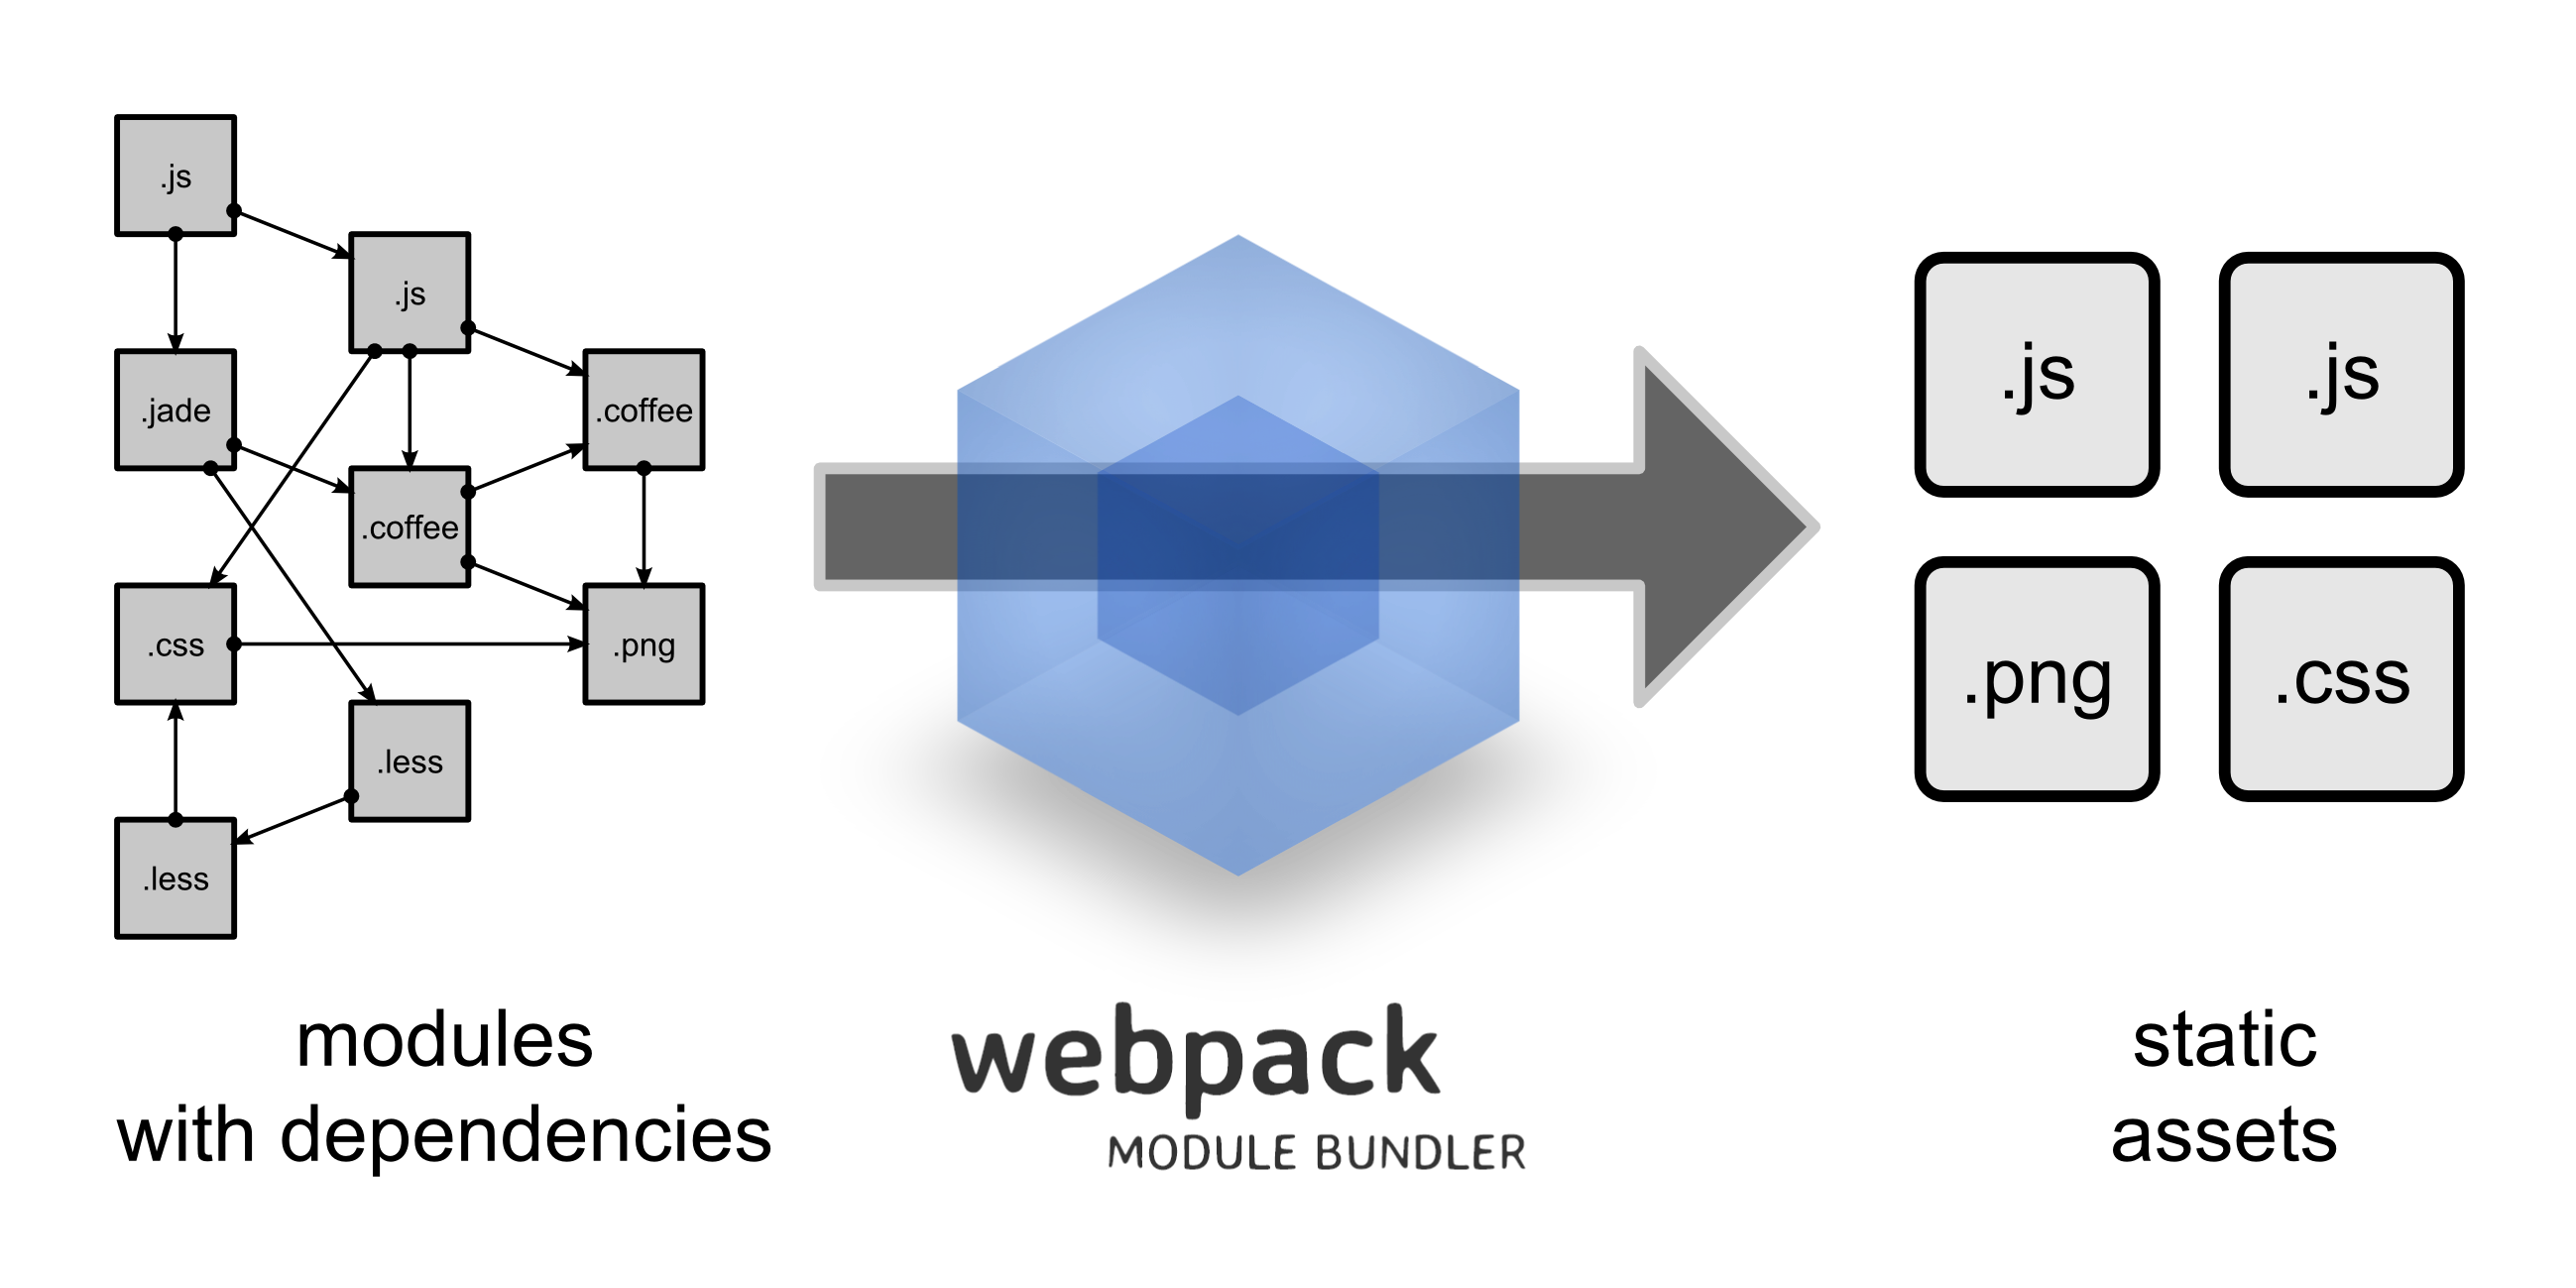
\includegraphics[width=\textwidth]{webpack.png}
    \caption{Zasada działania bundlera Webpack https://camo.githubusercontent.com/eac23581690c3ed7f73c0682aca8362fc0eff51ccd2700d28733f58936dd99d7/68747470733a2f2f7765627061636b2e6769746875622e696f2f6173736574732f776861742d69732d7765627061636b2e706e67}
    \label{fig:ast}
\end{figure}

W przypadku dużych projektów proces ten może być bardzo czasochłonny. Wraz z rozwojem ekosystemu JavaScript pojawiła się możliwość stosowania dynamicznych modułów ESM. Narzędziem wykorzystującym tę technikę jest Vite, które pozwala na szybkie budowanie i uruchamianie aplikacji React\cite{ViteSite}. Vite ładuje kod dynamicznie, co pozwala na pominięcie nieużywanych fragmentów w pamięci. Dzięki wsparciu dla HMR (Hot Module Reload) w środowisku deweloperskim, po wprowadzeniu drobnej zmiany nie trzeba budować całej aplikacji od nowa, co znacząco przyspiesza pracę.

W tej części porównano czas uruchamiania serwera deweloperskiego oraz budowania aplikacji.

Aplikacja korzystająca z CRA została stworzona za pomocą następujących komend:

\begin{lstlisting}[caption=Stworzenie i włączenie aplikacji React (CRA)]
npx create-react-app frontend-cra
cd frontend-cra
npm run start
\end{lstlisting}

Aplikację korzystającą z Vite stworzono używając: 

\begin{lstlisting}[caption=Stworzenie i włączenie aplikacji React (CRA)]
npm create vite@latest frontend-vite -- --template react-ts
cd frontend-vite
npm run dev
\end{lstlisting}

Obie aplikacje na starcie miały około 200 linijek kodu. W celu dalszych testów rozszerzono je do około 10,000 linijek kodu. Poniższe zestawienia przedstawiają czasy poszczególnych operacji.

\begin{table}[H]
\centering
\begin{tabular}{|l|l|l|}
\hline
\textbf{Operacja} & \textbf{Liczba linijek} & \textbf{Czas wykonania (s)} \\ \hline
\multirow{2}{*}{Włączenie serwera deweloperskieogo} & 200 & 10 \\ 
& 10,000 & 39 \\ \hline
\multirow{2}{*}{Zbudowanie aplikacji} & 200 & 19 \\ 
& 10,000 & 50 \\ \hline
\end{tabular}
\caption{Czasy operacji dla CRA}
\label{tab:czas_wykonania}
\end{table}

\begin{table}[H]
\centering
\begin{tabular}{|l|l|l|}
\hline
\textbf{Operacja} & \textbf{Liczba linijek} & \textbf{Czas wykonania (s)} \\ \hline
\multirow{2}{*}{Włączenie serwera deweloperskieogo} & 200 & 2 \\ 
& 10,000 & 3 \\ \hline
\multirow{2}{*}{Zbudowanie aplikacji} & 200 & 5 \\ 
& 10,000 & 8 \\ \hline
\end{tabular}
\caption{Czasy operacji dla Vite}
\label{tab:czas_wykonania}
\end{table}


Poniżej czasy zestawione na wykresie:


\begin{figure}[H]
\centering
\begin{tikzpicture}
\begin{axis}[
    title={Porównanie czasów operacji dla CRA i Vite},
    xlabel={Liczba linijek},
    ylabel={Czas wykonania (s)},
    xmin=0, xmax=10500,
    ymin=0, ymax=55,
    xtick={200,10000},
    ytick={0,10,20,30,40,50},
    legend pos=north west,
    ymajorgrids=true,
    grid style=dashed,
    scaled y ticks=false,
    scaled x ticks=false,
]

\addplot[
    color=blue,
    mark=square,
    ]
    coordinates {
    (200,10)(10000,39)
    };
\addlegendentry{CRA - Włączenie serwera}

\addplot[
    color=blue,
    mark=triangle,
    ]
    coordinates {
    (200,19)(10000,50)
    };
\addlegendentry{CRA - Zbudowanie aplikacji}

\addplot[
    color=red,
    mark=square,
    ]
    coordinates {
    (200,2)(10000,3)
    };
\addlegendentry{Vite - Włączenie serwera}

\addplot[
    color=red,
    mark=triangle,
    ]
    coordinates {
    (200,5)(10000,8)
    };
\addlegendentry{Vite - Zbudowanie aplikacji}

\end{axis}
\end{tikzpicture}
\caption{Porównanie czasów operacji dla CRA i Vite}
\label{fig:cra_vs_vite}
\end{figure}

Z badań wynika, że Vite oferuje znaczne przyspieszenie procesu budowania. Co istotne, zwiększenie liczby linijek kodu nie wpływa znacząco na czas wykonania operacji, co oznacza, że im większy projekt, tym bardziej widoczna staje się przewaga Vite.

W ciągu ostatnich lat zainteresowanie Vite wykazało dynamiczny wzrost, co znajduje odzwierciedlenie w danych Google Trends. Jak wskazuje praca Bhabishya Gurung\cite{babisha}, do około 2023 roku Create React App (CRA) dominowało w wynikach popularności wśród deweloperów. Jednak od tego momentu zauważalny jest wyraźny spadek zainteresowania CRA, podczas gdy Vite zdobywa coraz większą popularność. Zmiana ta może być związana z przewagami Vite w kontekście szybkości budowania i skalowalności, co czyni go bardziej atrakcyjnym dla dużych projektów i zaawansowanych aplikacji internetowych.

\subsection{Podsumowanie}

Powyższe badania pokazują, że domyślne narzędzia nie zawsze są optymalne. Optymalizację DevOps warto rozpocząć od wyboru odpowiednich narzędzi jeszcze przed rozpoczęciem projektu, gdyż zmiana tych narzędzi na późniejszych etapach może być czasochłonna i kosztowna.

\section{Metody wdrażania} \label{sectionMetodyWdrazania}

Po zbudowaniu aplikacji konieczne jest przeniesienie jej kodu na serwer oraz jej uruchomienie. Poniżej przedstawiono ogólne metody wdrażania, które zostaną szczegółowo opisane w kolejnych sekcjach:

\begin{itemize}
    \item całkowicie ręczne wdrażanie na serwer – deweloper uzyskuje dostęp do serwera, pobiera kod, instaluje potrzebne zależności i uruchamia aplikację,
    \item ręczne wdrażanie z dodatkiem – deweloper wykonuje czynności ręcznie, jednak nad działaniem aplikacji czuwa odpowiedni framework, np. \textbf{Nodemon} dla aplikacji NodeJS\cite{NodemonArticle},
    \item manualna wirtualizacja – deweloper samodzielnie buduje obraz, przesyła go do repozytorium artefaktów, a następnie uruchamia go na serwerze,
    \item automatyczna wirtualizacja – istnieje proces, który po wprowadzeniu zmian automatycznie buduje obraz i wdraża go na serwer.
\end{itemize}

Wszystkie powyższe techniki zakładają, że deweloper ma dostęp do serwera poprzez SSH, a sam serwer jest uwierzytelniony do repozytorium kodu.

\subsection{Całkowicie ręczne wdrażanie}

W tej metodzie deweloper ręcznie uruchamia aplikację na serwerze, podejmując większość kroków wykonywanych wcześniej w środowisku lokalnym, oraz zapewnia, że serwer poprawnie obsługuje zapytania przychodzące z zewnątrz.

Pierwsza konfiguracja może być szczególnie pracochłonna, obejmując pobranie i konfigurację narzędzi potrzebnych do budowania i wdrażania aplikacji w danej technologii (np. npm dla NodeJS). Występuje również ryzyko, że niektóre zależności potrzebne do działania aplikacji były zainstalowane globalnie na komputerze dewelopera, co może prowadzić do problemów w działaniu aplikacji na serwerze.

W książce "Continuous Delivery: Reliable Software Releases through Build, Test, and Deployment Automation" \cite{continuousDelivery} autorzy Jez Humble i David Farley opisują tradycyjne podejście do wdrażania aplikacji, gdzie deweloperzy ręcznie kopiują kod na serwer, instalują zależności i uruchamiają aplikację. Podkreślają, że takie podejście jest podatne na błędy i trudne do skalowania.

\begin{figure}[H]
    \centering
    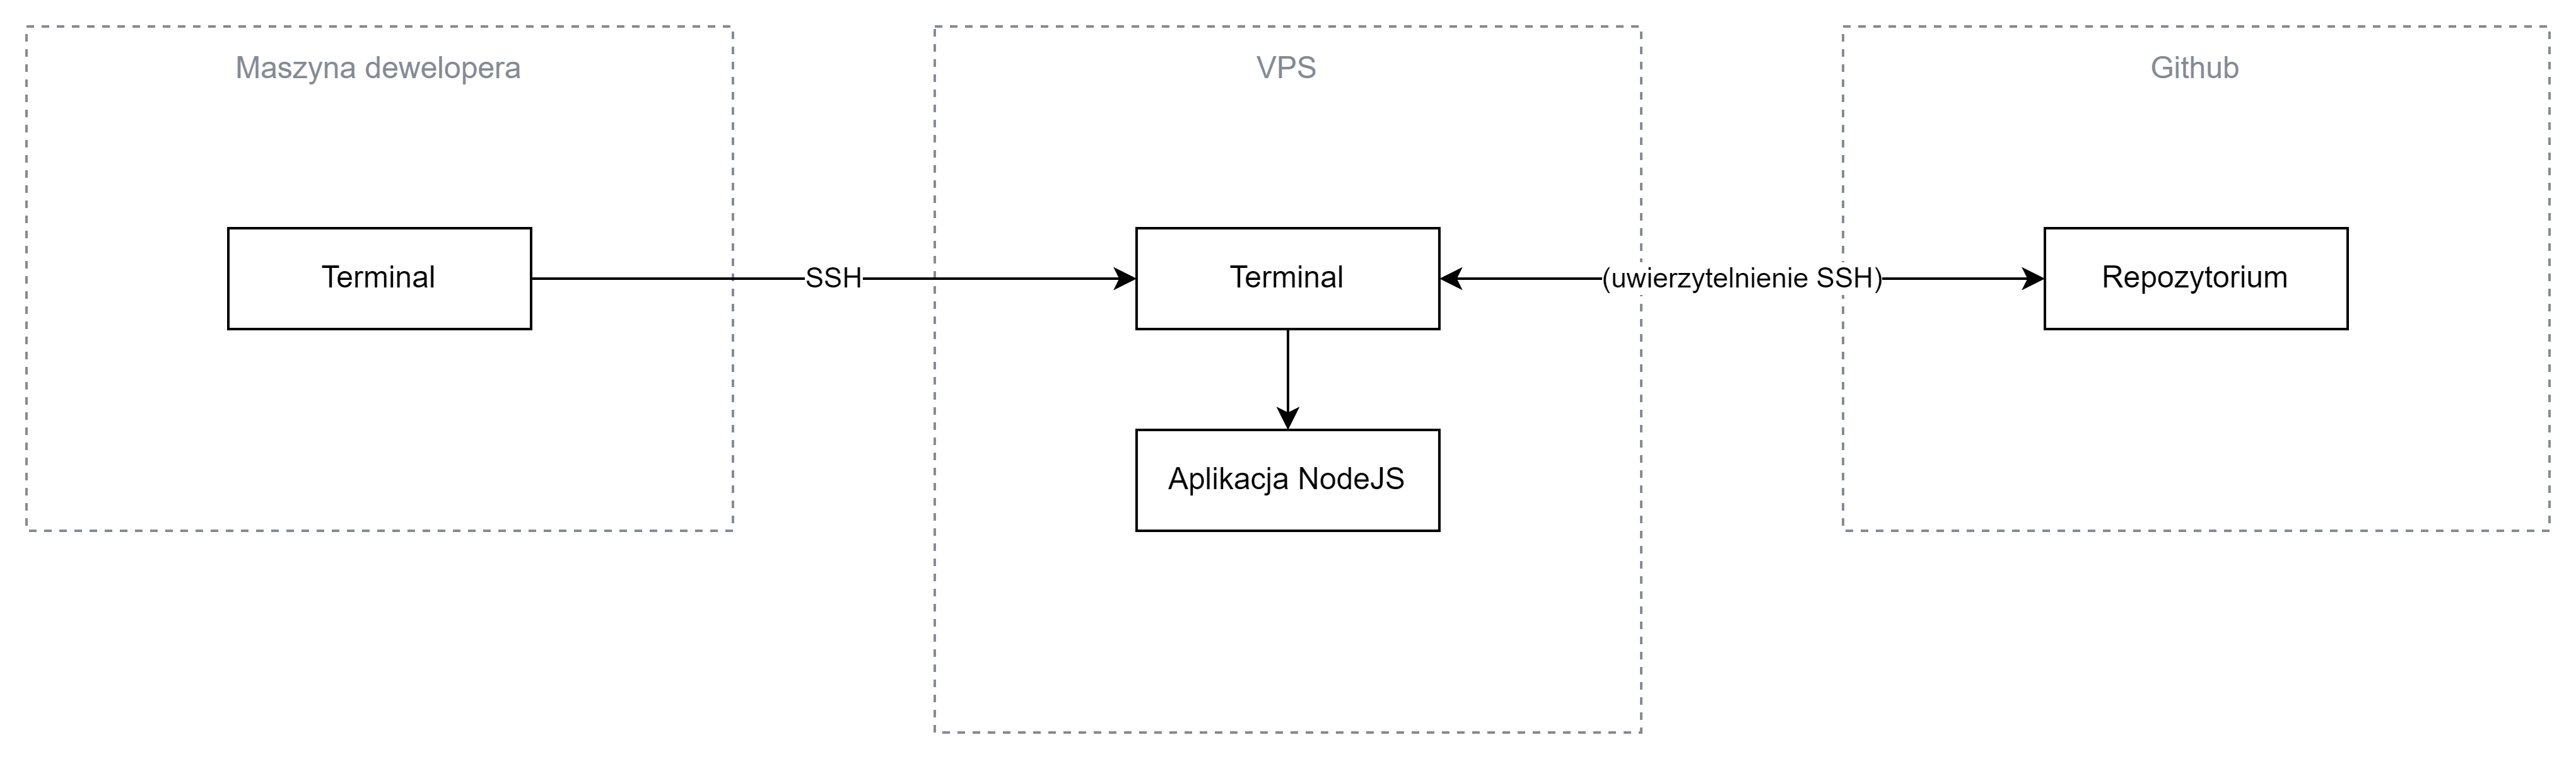
\includegraphics[width=1\linewidth]{reczne_wdrazanie.png}
    \caption{Całkowicie ręczne wdrażanie}
    \label{fig:enter-label}
\end{figure}

\begin{itemize}
    \item pobranie nowej wersji kodu,
    \item zainstalowanie potrzebnych zależności,
    \item zatrzymanie starej wersji aplikacji,
    \item włączenie nowej wersji aplikacji
\end{itemize}

\subsubsection{Zalety}

\begin{itemize}
    \item brak potrzeby konfiguracji narzędzi automatyzujących, co sprawia, że pierwsze wdrożenie jest szybkie.
\end{itemize}

\subsubsection{Wady}

\begin{itemize}
    \item czasochłonność związana z powtarzaniem ręcznych czynności przy każdym wdrożeniu,
    \item możliwość wystąpienia problemów wynikających z różnic w konfiguracji środowiska,
    \item brak możliwości monitorowania aplikacji,
    \item brak zarządzania stanem aplikacji brak zarządzania stanem aplikacji (po restarcie serwera lub błędzie aplikacja pozostaje wyłączona),
    \item bezpośredni dostęp do systemu operacyjnego hosta.
\end{itemize}

\subsection{Ręczne wdrażanie z dodatkiem}

W tej metodzie wdrożenie wspomaga dodatkowe narzędzie, np. Nodemon, które wprowadza warstwę abstrakcji dla aplikacji NodeJS. Nodemon zarządza stanem aplikacji, monitorując jej "zdrowie", umożliwia skalowanie oraz automatyczny load balancing.

W swojej pracy \cite{characterizationFramework} Carzaniga, Fugetta, Hall oraz Heimbigner przedstawiają technologie wspierające proces wdrażania aplikacji, podkreślając znaczenie narzędzi, które pomagają zarządzać wdrożeniem i jego etapami. Opisują, jak narzędzia te umożliwiają bardziej efektywne wdrażanie aplikacji przez automatyzację powtarzalnych zadań, takich jak kopiowanie plików czy konfiguracja serwera. Dzięki temu proces staje się mniej podatny na błędy i łatwiejszy do kontrolowania. Autorzy zwracają uwagę, że użycie takich technologii pozwala na szybsze i bardziej spójne wdrażanie, co jest kluczowe w przypadku dużych i dynamicznych środowisk, gdzie aktualizacje muszą być wprowadzane regularnie.

\begin{figure}[H]
    \centering
    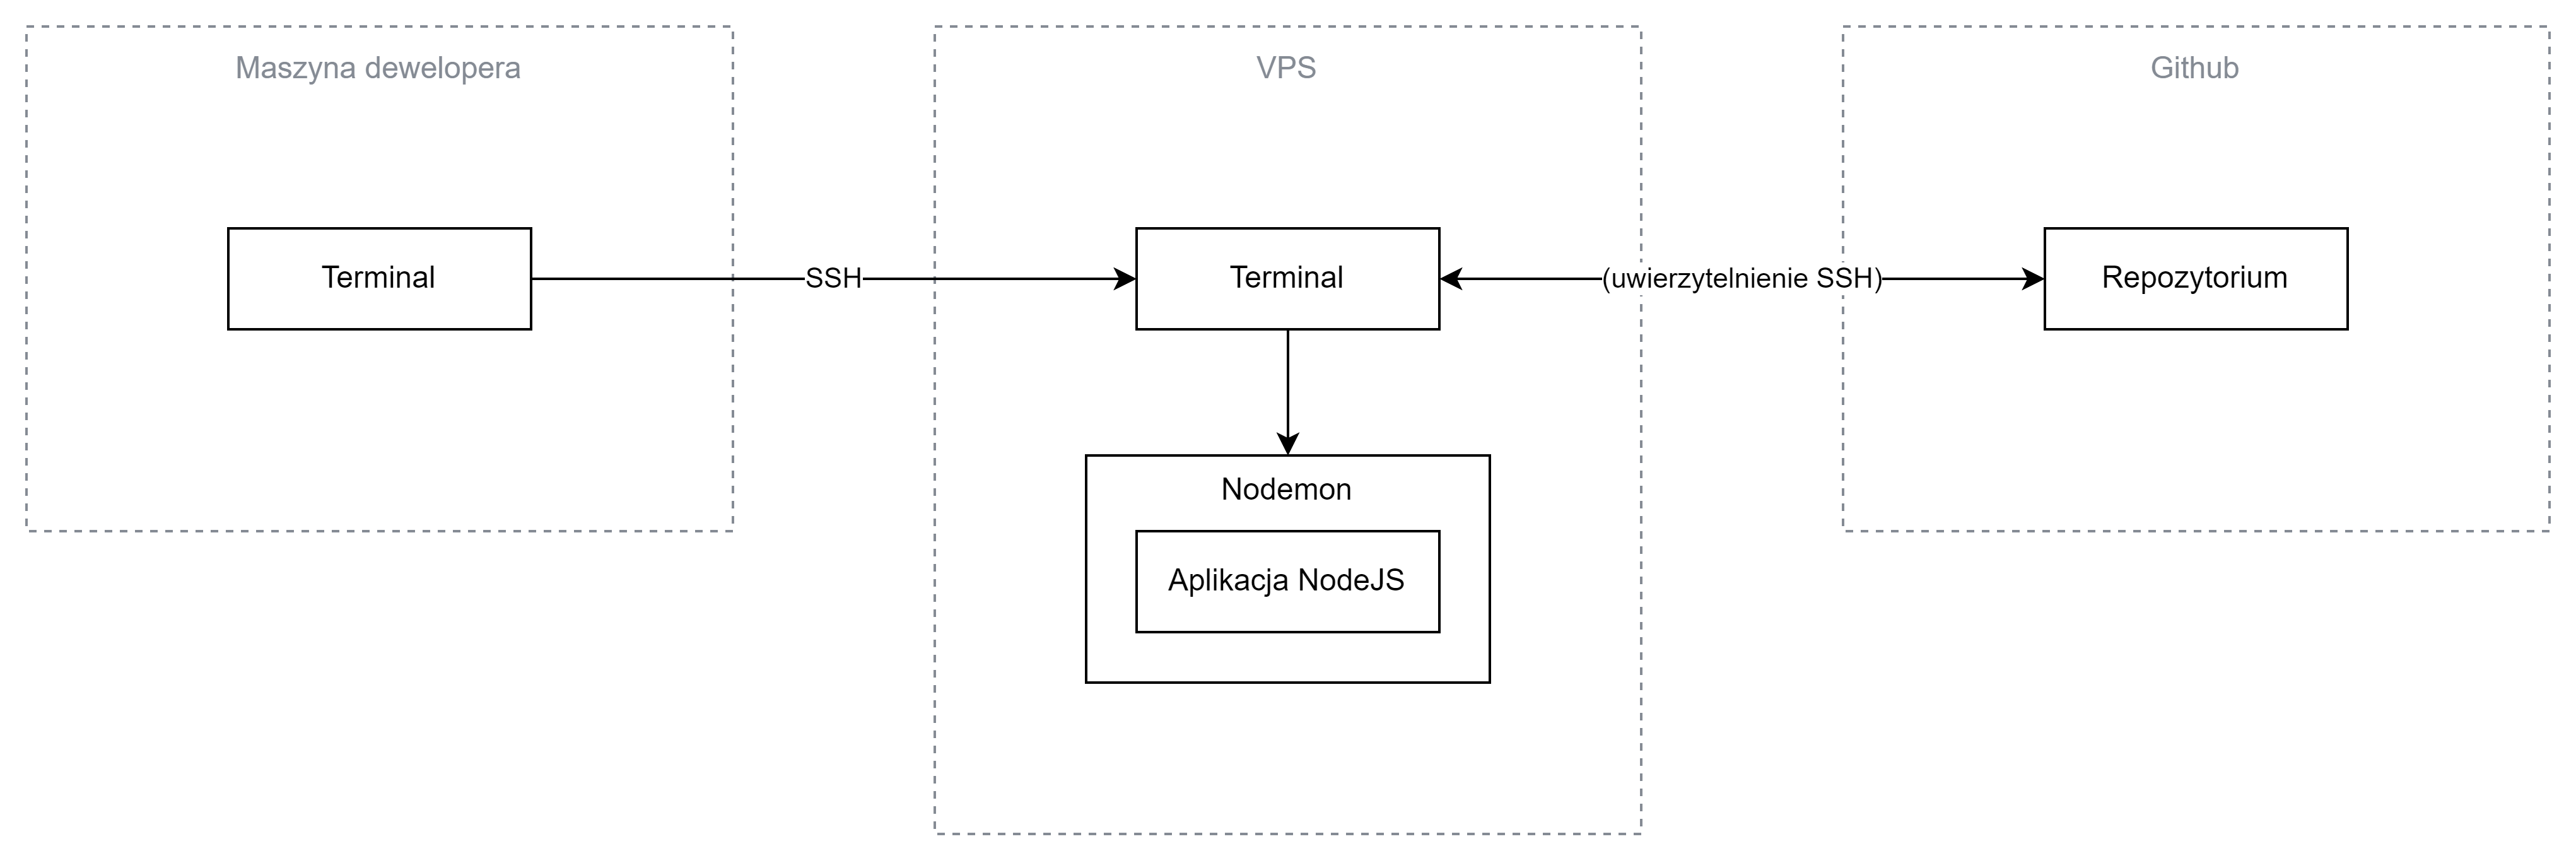
\includegraphics[width=1\linewidth]{reczneWdrazanieZDodatkiem.png}
    \caption{Ręczne wdrażanie z dodatkiem}
    \label{fig:enter-label}
\end{figure}

\subsubsection{Zalety}

\begin{itemize}
    \item podstawowe monitorowania aplikacji,
    \item zarządzanie stanem aplikacji (automatyczne restartowanie, jeśli wystąpi taka potrzeba),
    \item możliwość prostego skalowania oraz automatyczny load balancing.
\end{itemize}

\subsubsection{Wady}

\begin{itemize}
    \item aplikacja nadal narażona jest na różnice w konfiguracji środowiska,
    \item aplikacja nadal ma bezpośredni dostęp do systemu operacyjnego hosta.
\end{itemize}

\subsection{Manualna wirtualizacja}

W tej metodzie deweloper ręcznie buduje obraz na komputerze lokalnym i wysyła go do repozytorium artefaktów. Następnie loguje się na serwerze, pobiera obraz i uruchamia kontener z nową wersją aplikacji.

\begin{figure}[H]
    \centering
    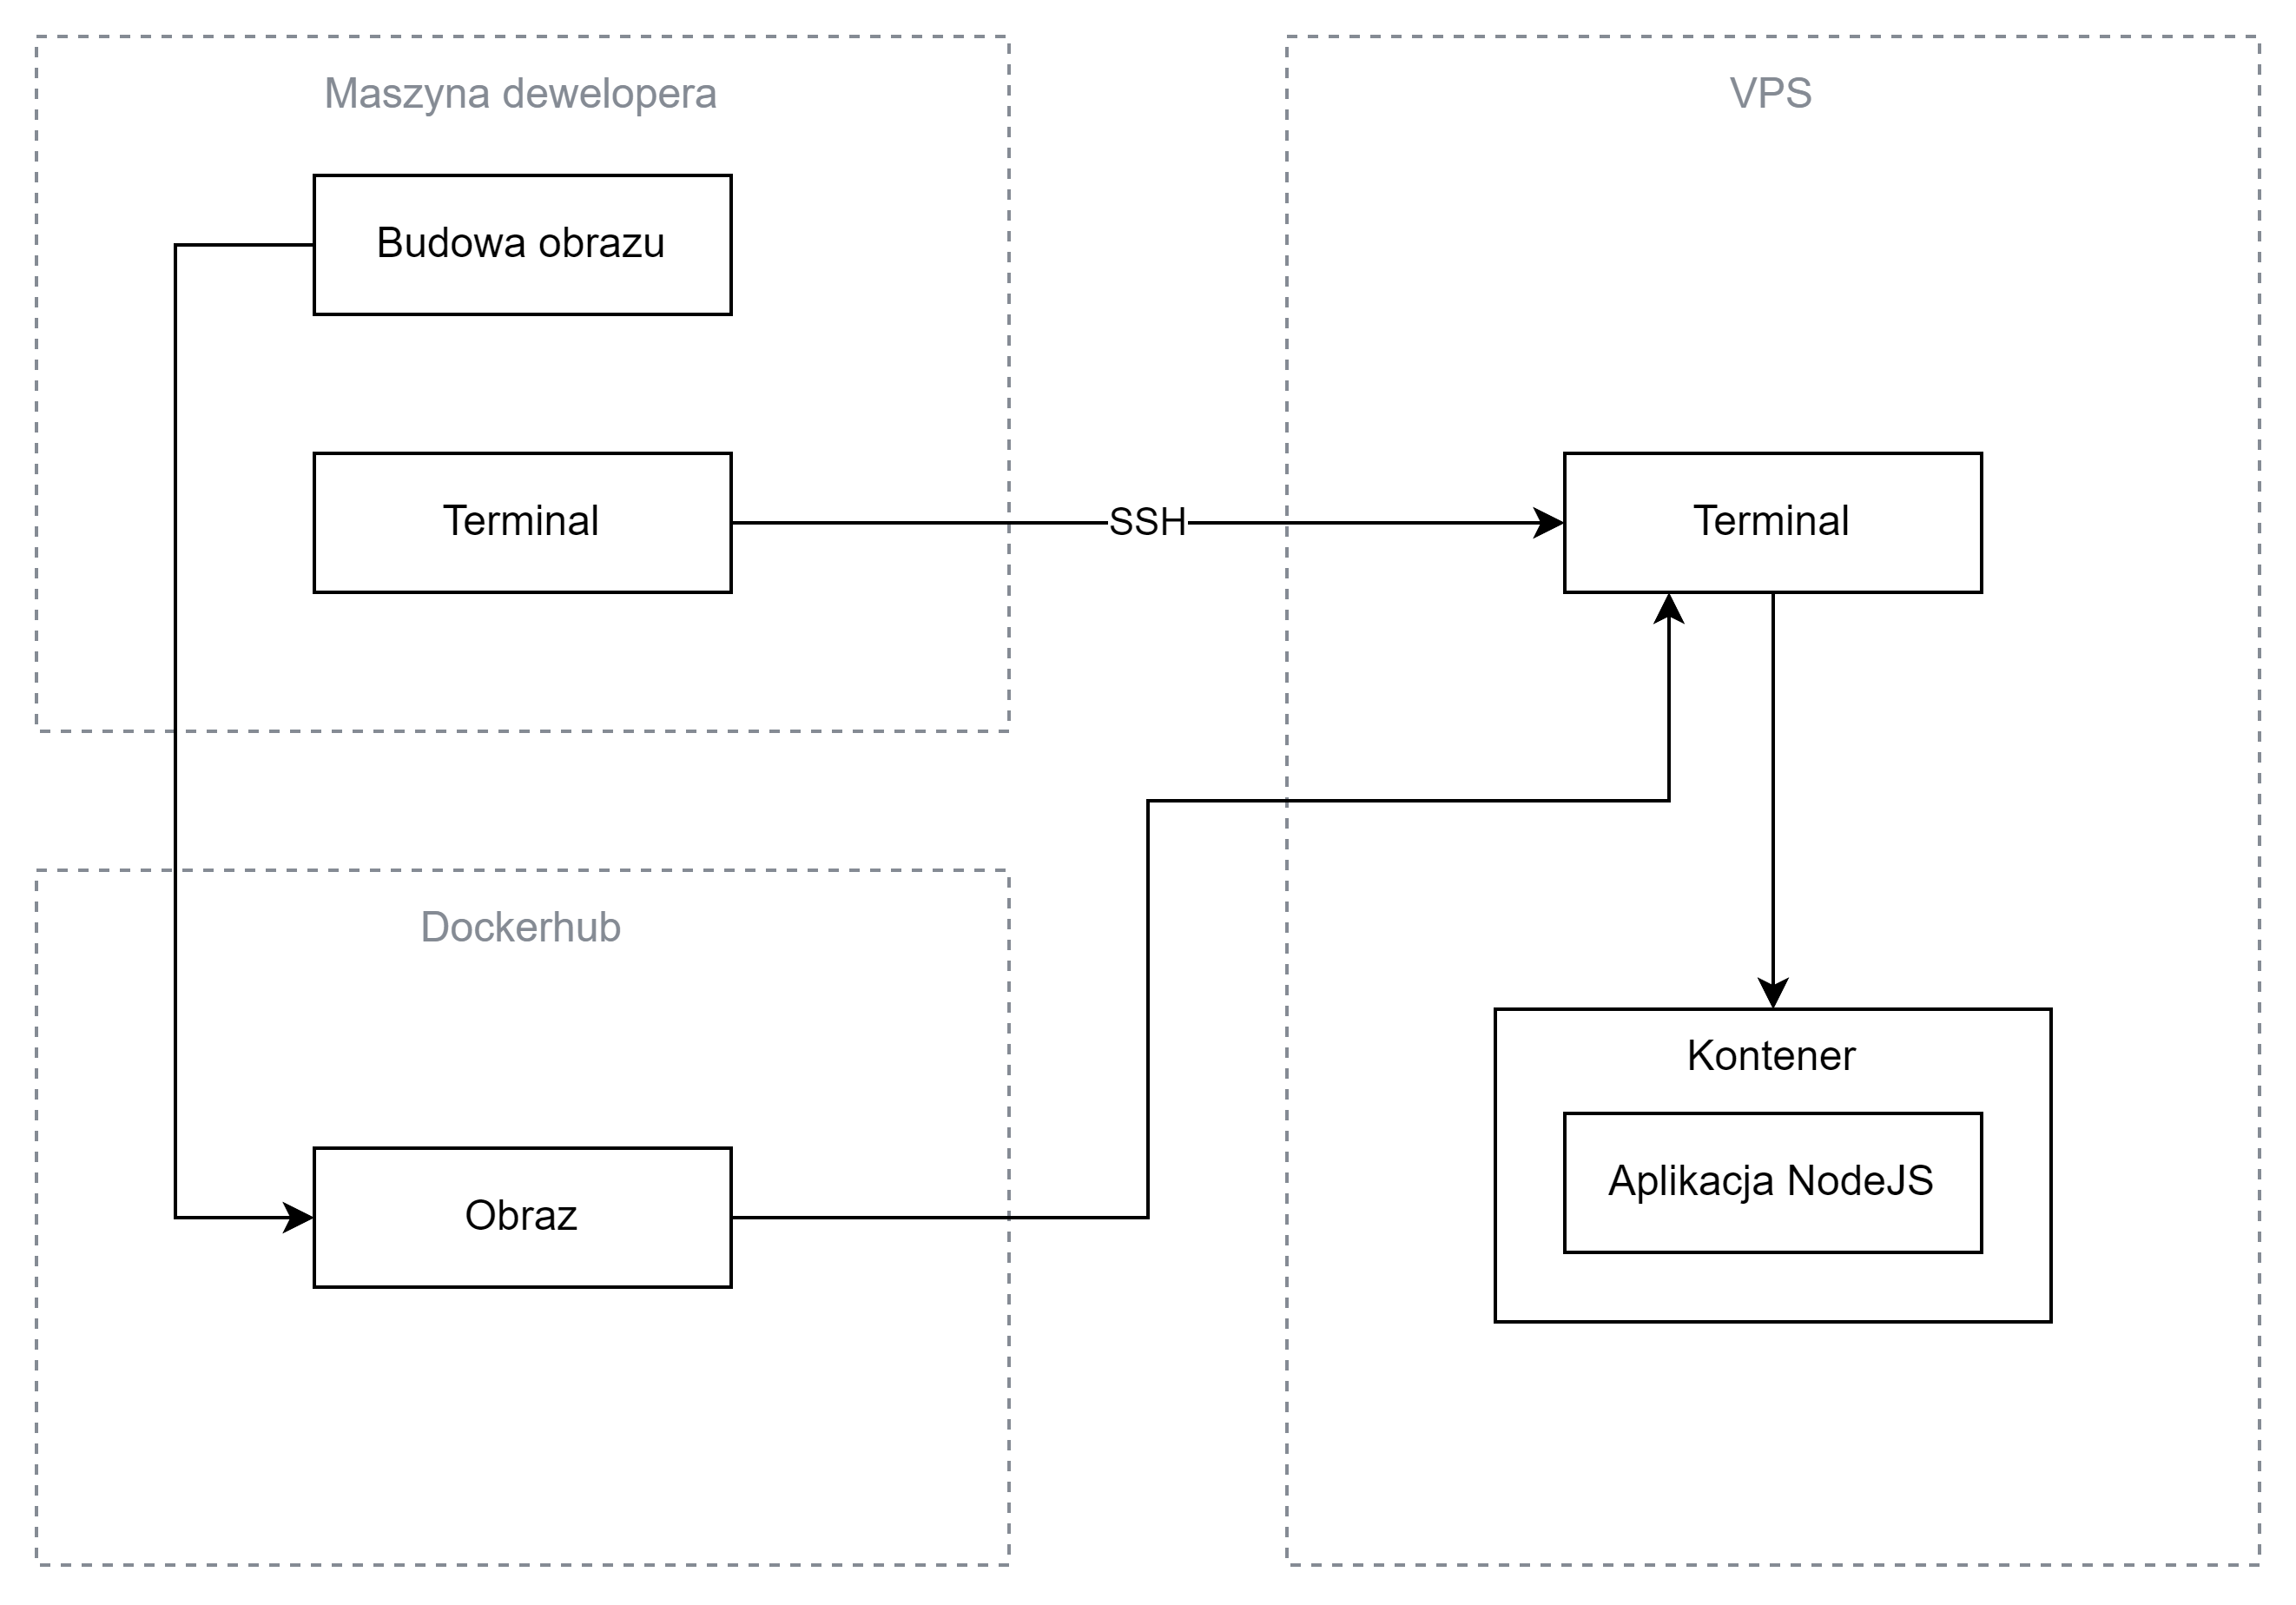
\includegraphics[width=1\linewidth]{manualnaWirtualizacja.png}
    \caption{Manualna wirtualizacja}
    \label{fig:enter-label}
\end{figure}

\subsubsection{Zalety}

\begin{itemize}
    \item szybsza konfiguracja środowiska, wymagająca jedynie narzędzi do obsługi wirtualizacji na serwerze,
    \item zredukowane ryzyko błędów wynikających z różnic w konfiguracji. Deweloper może przetestować obraz lokalnie,
    \item brak dostępu aplikacji do systemu operacyjnego hosta.
\end{itemize}

\subsubsection{Wady}

\begin{itemize}
    \item skomplikowanie infrastruktury projektu - konieczność utrzymania repozytorium obrazów,
    \item trudność wprowadzenia zmian w konfiguracji aplikacji, zwłaszcza dla deweloperów bez doświadczenia poza kodem samej aplikacji,
\end{itemize}

\subsection{Wirtualizacja + CI/CD}

W tym podejściu wdrażanie jest w pełni zautomatyzowane dzięki infrastrukturze CI/CD. Po wprowadzeniu zmian w repozytorium agent CI/CD automatycznie uruchamia się, buduje obraz i wdraża go na serwer, uruchamiając kontener z nową wersją aplikacji.

\begin{figure}[H]
    \centering
    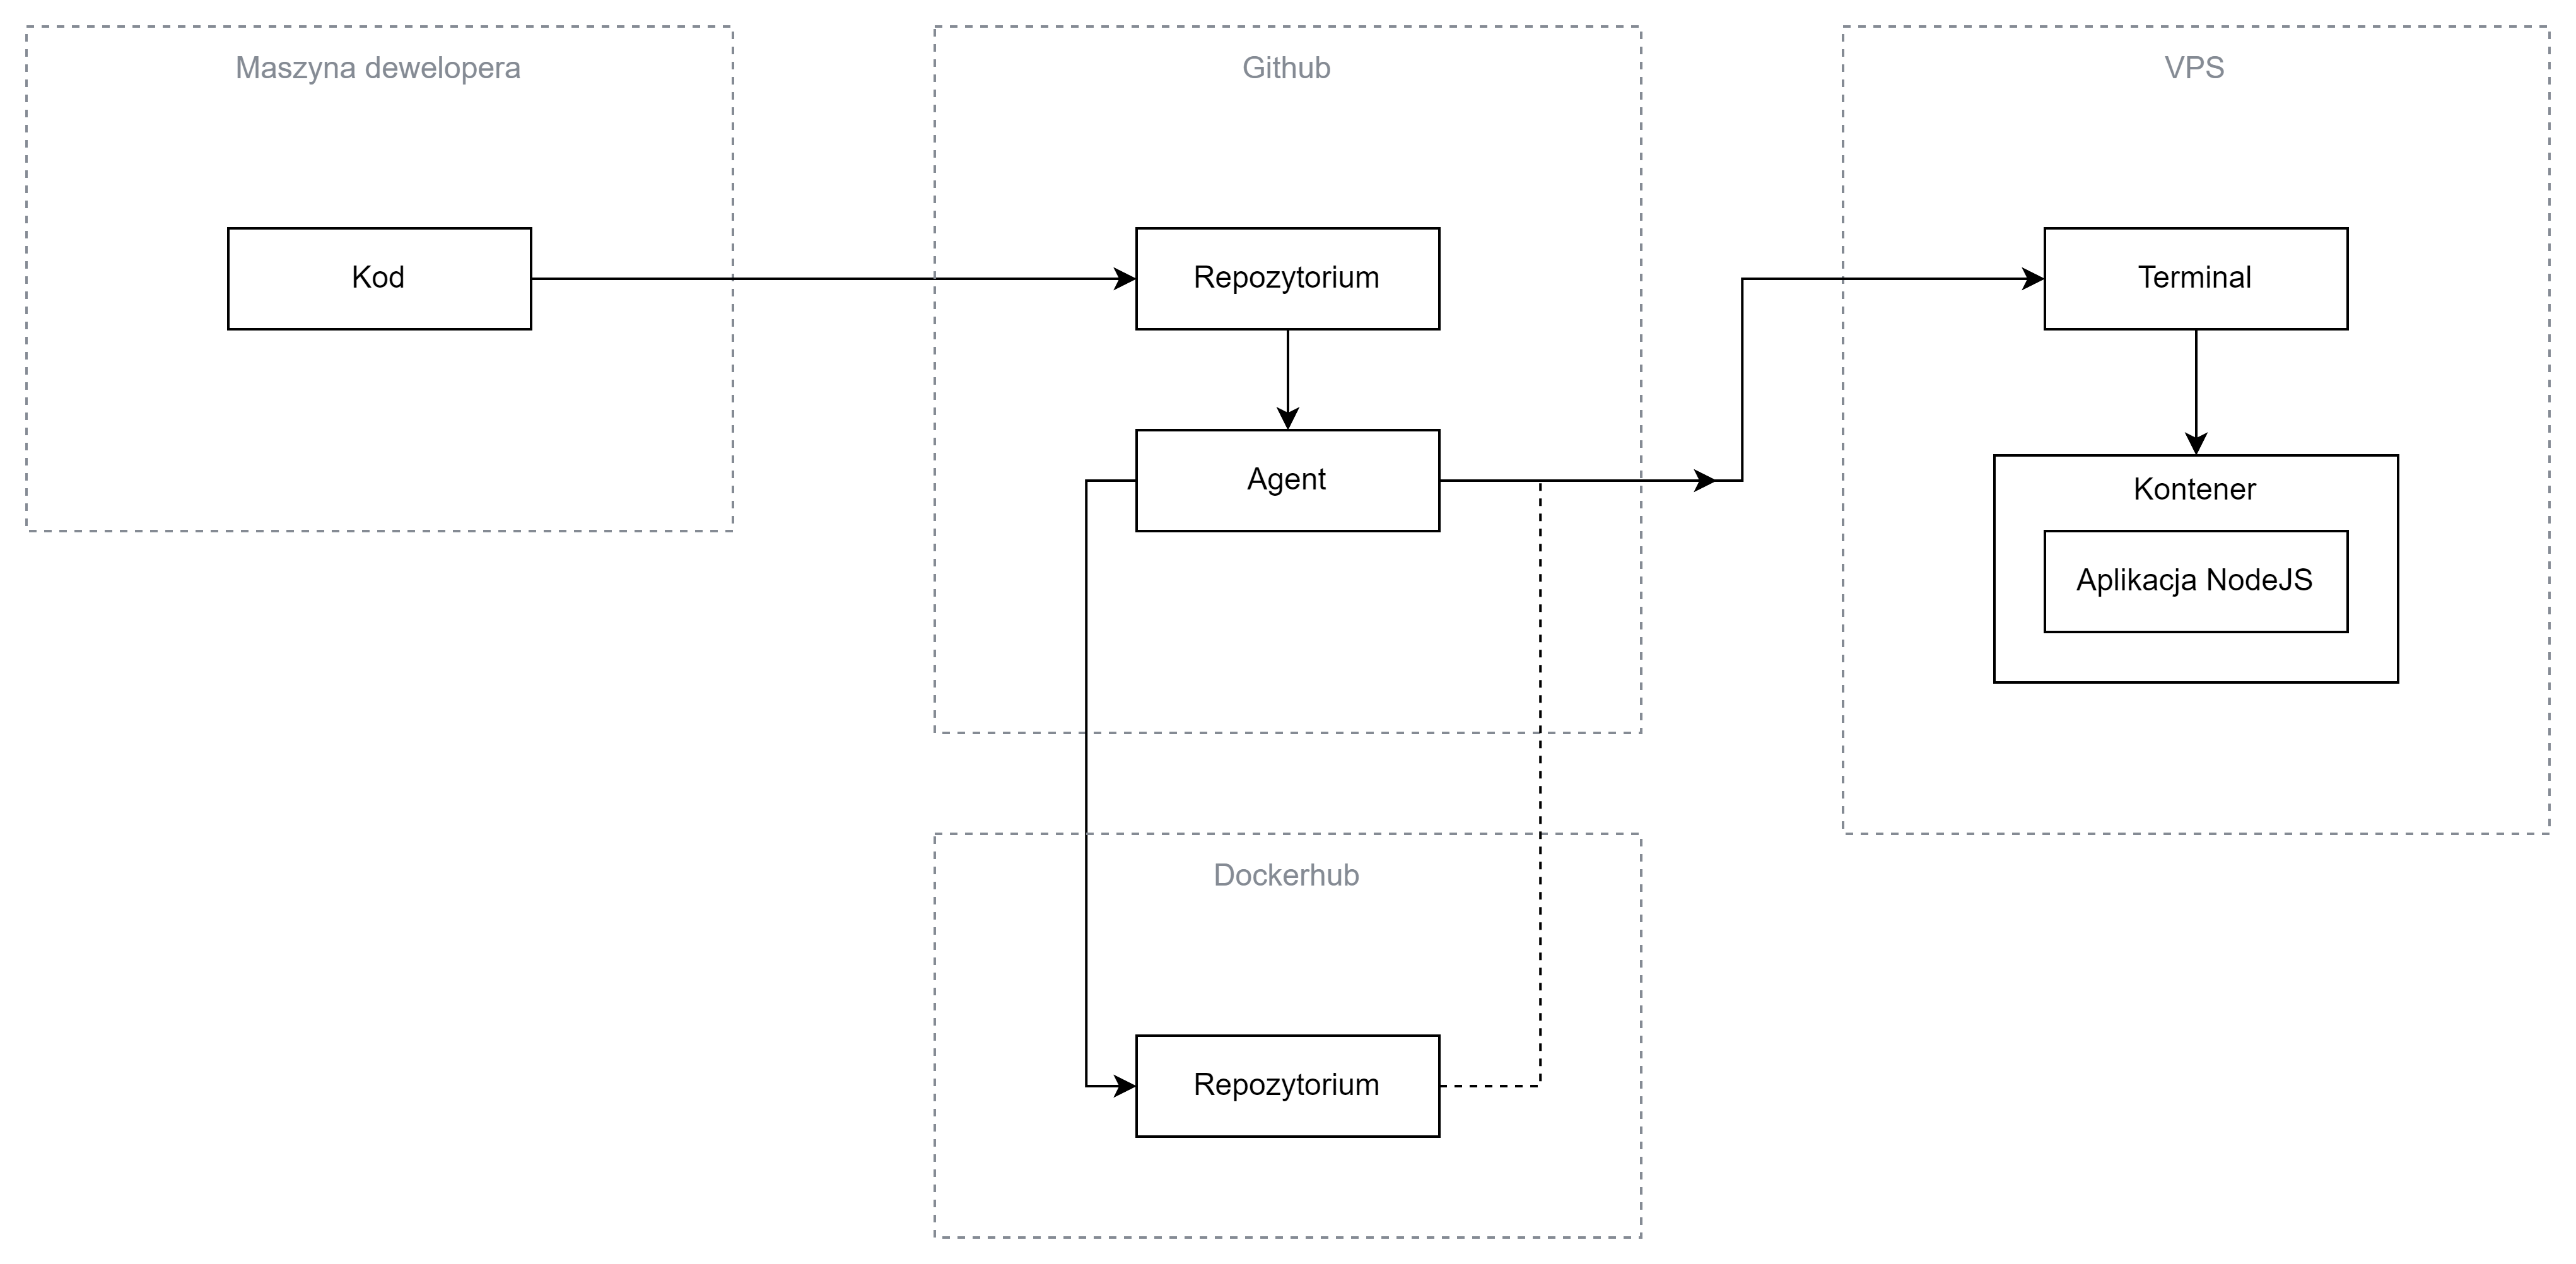
\includegraphics[width=1\linewidth]{automatycznaWirtualizacja.png}
    \caption{Wirtualizacja + CI/CD}
    \label{fig:enter-label}
\end{figure}

\subsubsection{Zalety}

\begin{itemize}
    \item znaczące usprawnienie procesu wdrażania aplikacji,
    \item minimalizacja błędów konfiguracji,
    \item łatwe rozszerzenie na wiele środowisk.
\end{itemize}

\subsubsection{Wady}

\begin{itemize}
    \item znaczne skomplikowanie infrastruktury projektu. Potrzeba wybrania narzędzia do CI/CD oraz tworzenia i utrzymywania plików konfiguracyjnych,
\end{itemize}

\subsection{Podsumowanie}

\textbf{Podatność na błędy konfiguracji}
\begin{itemize}
    \item \textbf{całkowicie ręczne wdrażanie} - wysoka podatność na błędy konfiguracji wynikająca z ręcznego wprowadzania ustawień, co zwiększa ryzyko pomyłek ludzkich, takich jak literówki, niezgodność wersji czy pominięcie kroków konfiguracji,
    \item \textbf{ręczne wdrażanie z dodatkami} - nadal wysoka podatność na błędy, ponieważ kluczowe etapy konfiguracji wciąż są wykonywane ręcznie, mimo użycia dodatkowych narzędzi wspomagających,
    \item \textbf{wirtualizacja} - Niska podatność dzięki możliwości definiowania konfiguracji w formie szablonów (np. plików YAML) oraz automatyzacji części procesu,
    \item \textbf{wirtualizacja + CI/CD} - bardzo niska podatność na błędy dzięki pełnej automatyzacji i standaryzacji procesów konfiguracji, co minimalizuje interwencje manualne.
\end{itemize}

\textbf{Czas potrzebny na pierwszą konfigurację}
\begin{itemize}
    \item \textbf{całkowicie ręczne wdrażanie} - niski, ponieważ proces ogranicza się do manualnego uruchomienia aplikacji i podstawowej konfiguracji środowiska na serwerze,
    \item \textbf{Ręczne wdrażanie z dodatkami} - średni, ponieważ korzystanie z dodatkowych narzędzi (np. skryptów) wymaga ich wcześniejszego przygotowania i dostosowania do specyfiki środowiska,
    \item \textbf{wirtualizacja} - wysoki, gdyż przygotowanie infrastruktury wirtualizacyjnej wymaga szczegółowego zaplanowania, instalacji oprogramowania (np. Docker, Kubernetes) i utworzenia odpowiednich szablonów,
    \item \textbf{wirtualizacja + CI/CD}: bardzo wysoki, ponieważ wdrożenie wymaga skonfigurowania zarówno wirtualizacji, jak i narzędzi CI/CD, takich jak Jenkins, GitLab CI czy GitHub Actions, co może być czasochłonne.
\end{itemize}

\textbf{Czas wdrożenia nowej wersji aplikacji}
\begin{itemize}
    \item \textbf{całkowicie ręczne wdrażanie} - wysoki, ponieważ każda aktualizacja wymaga ręcznego przesłania plików na serwer i ponownej konfiguracji środowiska.
    \item \textbf{ręczne wdrażanie z dodatkami} - wysoki, mimo pewnych udogodnień (np. skrypty automatyzujące część procesu), proces nadal wymaga ręcznej ingerencji.
    \item \textbf{Wirtualizacja} - średni, dzięki możliwości szybkiego odtwarzania środowiska aplikacji z wykorzystaniem obrazów kontenerów,
    \item \textbf{wirtualizacja + CI/CD}: niski, gdyż cały proces wdrożenia nowej wersji aplikacji jest zautomatyzowany i wykonywany w ciągu kilku minut od zgłoszenia zmiany.
\end{itemize}

\textbf{Zarządzanie stanem aplikacji}
\begin{itemize}
    \item \textbf{całkowicie ręczne wdrażanie} - brak możliwości zarządzania stanem aplikacji poza manualnym podejściem, co zwiększa ryzyko niespójności,
    \item \textbf{ręczne wdrażanie z dodatkami}: możliwość częściowego zarządzania stanem aplikacji za pomocą dodatkowych narzędzi, takich nodemon,
    \item \textbf{wirtualizacja} - automatyczne zarządzanie stanem aplikacji poprzez obrazy kontenerów i pliki konfiguracyjne,
    \item \textbf{wirtualizacja + CI/CD} - pełna automatyzacja zarządzania stanem aplikacji, integrująca kontrolę wersji, konfigurację środowiska i logikę aplikacji w jednym procesie.
\end{itemize}

\textbf{Skalowanie aplikacji}
\begin{itemize}
    \item \textbf{całkowicie ręczne wdrażanie} - skalowanie aplikacji jest bardzo trudne, ponieważ wymaga manualnego uruchamiania dodatkowych instancji aplikacji i konfiguracji środowiska na każdym serwerze,
    \item \textbf{ręczne wdrażanie z dodatkami} - skalowanie jest łatwiejsze niż w przypadku całkowicie ręcznego wdrażania, dzięki wykorzystaniu narzędzi automatyzujących niektóre kroki. Jednak wciąż wymaga ręcznego dostosowywania konfiguracji,
    \item \textbf{wirtualizacja} - skalowanie jest proste dzięki możliwości uruchamiania wielu instancji aplikacji w formie kontenerów na jednej lub wielu maszynach fizycznych,
    \item \textbf{wirtualizacja + CI/CD} - skalowanie jest bardzo łatwe i zautomatyzowane, szczególnie w połączeniu z systemami zarządzania orkiestracją kontenerów, takimi jak Kubernetes, co pozwala na dynamiczne dostosowywanie liczby instancji do aktualnego obciążenia.
\end{itemize}

\textbf{Podatność na ataki}
\begin{itemize}
    \item \textbf{całkowicie ręczne wdrażanie} - wysoka podatność na ataki wynikająca z braku standaryzacji i automatyzacji. Ręcznie skonfigurowane środowiska często zawierają błędy bezpieczeństwa, takie jak otwarte porty czy przestarzałe wersje oprogramowania,
    \item \textbf{ręczne wdrażanie z dodatkami}: podatność na ataki pozostaje wysoka, ponieważ dodatkowe narzędzia nie eliminują wszystkich luk bezpieczeństwa związanych z manualnym podejściem,
    \item \textbf{wirtualizacja} - niska podatność na ataki dzięki izolacji aplikacji w kontenerach oraz standaryzacji konfiguracji, co minimalizuje ryzyko wynikające z błędów ludzkich.
    \item \textbf{wirtualizacja + CI/CD} - bardzo niska podatność na ataki, ponieważ proces CI/CD uwzględnia automatyczne skanowanie bezpieczeństwa, aktualizację zależności i eliminację znanych luk w zabezpieczeniach na etapie budowania i wdrażania aplikacji.
\end{itemize}

\textbf{Monitorowanie aplikacji}
\begin{itemize}
    \item \textbf{całkowicie ręczne wdrażanie} - brak monitorowania aplikacji. Ewentualne problemy są wykrywane tylko w wyniku zgłoszeń użytkowników, co znacząco opóźnia reakcję na awarie,
    \item \textbf{ręczne wdrażanie z dodatkami} - monitorowanie wymaga ręcznej konfiguracji narzędzi lub skryptów, co ogranicza zakres i jakość zbieranych danych. Nadal pozostaje to wysoce zależne od manualnej pracy,
    \item \textbf{wirtualizacja} - Monitorowanie aplikacji jest możliwe dzięki wbudowanym funkcjom niektórych narzędzi wirtualizacyjnych (np. Docker Stats). Można łatwo zbierać dane o zasobach, takich jak CPU czy pamięć, ale bardziej zaawansowane monitorowanie wymaga dodatkowych narzędzi,
    \item \textbf{wirtualizacja + CI/CD} - pełne monitorowanie jest integralną częścią procesu, dzięki wykorzystaniu rozwiązań takich jak Prometheus, Grafana czy ELK Stack, które umożliwiają bieżące śledzenie wydajności, logów oraz stanu aplikacji w czasie rzeczywistym.
\end{itemize}

\begin{table}[H]
\centering
\begin{tabular}{|l|c|c|c|c|}
\hline
\textbf{Cecha} & \textbf{1} & \textbf{2} & \textbf{3} & \textbf{4} \\ \hline
Podatność na błędy konfiguracji         & \cellcolor{red!50}wysoka & \cellcolor{red!50}wysoka & \cellcolor{green!50}niska & \cellcolor{green!50}niska \\ \hline
Czas potrzebny na pierwszą konfigurację & \cellcolor{green!50}niski & \cellcolor{yellow!50}średni & \cellcolor{red!50}wysoki & \cellcolor{red!50}bardzo wysoki \\ \hline
Czas wdrożenia nowej wersji aplikacji   & \cellcolor{red!50}wysoki & \cellcolor{red!50}wysoki & \cellcolor{yellow!50}średni & \cellcolor{green!50}niski \\ \hline
Zarządzanie stanem aplikacji            & \cellcolor{red!50}nie & \cellcolor{green!50}tak & \cellcolor{green!50}tak & \cellcolor{green!50}tak \\ \hline
Skalowanie aplikacji                    & \cellcolor{red!50}trudne & \cellcolor{green!50}łatwe & \cellcolor{green!50}łatwe & \cellcolor{green!50}łatwe \\ \hline
Podatność na ataki                      & \cellcolor{red!50}wysoka & \cellcolor{red!50}wysoka & \cellcolor{green!50}niska & \cellcolor{green!50}niska \\ \hline
Monitorowanie aplikacji                 & \cellcolor{red!50}nie & \cellcolor{red!50}nie & \cellcolor{green!50}tak & \cellcolor{green!50}tak \\ \hline
\end{tabular}
\caption{Porównanie metod wdrażania: 1 - całkowicie ręczne, 2 - ręczne z dodatkiem, 3 - wirtualizacja, 4 - wirtualizacja + CI/CD}
\label{tab:porownanie-metod-wdrazania}
\end{table}

Zasadniczym plusem ręcznego wdrażania jest szybkość pierwszej konfiguracji. Konfiguracja upraszcza się do włączenia aplikacji na serwerze. Udowodniono jednak, że liczba zalet wirtualizacji z użyciem CI/CD przewyższa zysk czasowy manualnego wdrażania. Warto poświęcić na początku więcej czasu na dobrą konfigurację aby zaoszczędzić go w późniejszych fazach rozwoju aplikacji.


\section{Budowa obrazu} \label{sectionBudowaObrazu}

\subsection{Podstawowy obraz}

Analizę rozpoczęto od przygotowania najprostszego obrazu Dockerowego, zapewniającego jedynie poprawne działanie aplikacji. W tym celu do katalogu aplikacji dodano plik \textbf{Dockerfile} o poniższej zawartości:

\begin{lstlisting}[caption=Podstawowy plik Dockerfile]
FROM node:18

WORKDIR /usr/src/app

COPY package*.json ./

RUN npm install

COPY . .

RUN npm run build

CMD [ "node", "dist/main.js" ]
\end{lstlisting}

Z definicji pliku wynika, że wybiera on obraz bazowy, przenosi pliki konfiguracyjne, instaluje potrzebne zależności, przenosi pliki źródłowe, buduje aplikacje i ją włącza.

Z powyższej definicji wynika, że plik wybiera obraz bazowy, przenosi pliki konfiguracyjne, instaluje niezbędne zależności, kopiuje pliki źródłowe, buduje aplikację i uruchamia ją. Czas budowy obrazu wynosi \textbf{85 sekund}, a jego rozmiar to \textbf{1.64 GB}. Najwięcej czasu zajmuje krok \lstinline|[internal] load build context|.

\subsection{Dockerignore}

Warto zauważyć, że NodeJS przechowuje potrzebne zależności w katalogu z plikami projektu, co oznacza, że instrukcja \lstinline|COPY . .| w pliku Dockerfile przeniesie te zależności do obrazu, choć nie jest to konieczne, gdyż będą one pobrane w procesie budowy.

Aby uniknąć kopiowania zbędnych plików, stosuje się plik \lstinline|.dockerignore|, w którym można określić elementy ignorowane przez Docker podczas kopiowania.

\begin{lstlisting}[caption=Plik .dockerignore]
dist
node_modules
\end{lstlisting}

Oprócz katalogu z zależnościami, warto także wykluczyć katalog z plikami wynikowymi aplikacji, gdyż muszą one być zbudowane ponownie w obrazie. Po dodaniu pliku \lstinline|.dockerignore| czas budowy obrazu wynosi \textbf{24 sekundy}, a jego rozmiar zmniejszył się do \textbf{1.42 GB}.

\subsection{Multi stage build}

Node.js dzieli swoje zależności na produkcyjne oraz deweloperskie. Zależności produkcyjne są wymagane do działania aplikacji, natomiast deweloperskie, takie jak \textbf{TypeScript}, są potrzebne jedynie w fazie budowania\cite{NodejsAviary}.

\begin{lstlisting}[caption=Multistage plik Dockerfile]
FROM node:18 AS development
WORKDIR /usr/src/app
COPY package*.json ./
RUN npm ci -f
COPY . .


FROM node:18 AS build
WORKDIR /usr/src/app
COPY package*.json ./
COPY --from=development /usr/src/app/node_modules ./node_modules
COPY . .
RUN npm run build
RUN npm ci -f --only=production && npm cache clean --force


FROM node:18 AS production
ENV NODE_ENV production
COPY --from=build /usr/src/app/node_modules ./node_modules
COPY --from=build /usr/src/app/dist ./dist
CMD [ "node", "dist/main.js" ]
\end{lstlisting}

Powyższy plik \lstinline|Dockerfile| definiuje trójetapowy proces budowy:

\begin{enumerate}
    \item development - instaluje zależności i kopiuje pliki źródłowe do obrazu,
    \item build - kopiuje zależności z pierwszego etapu, buduje aplikację, a następnie usuwa zależności deweloperskie,
    \item production - kopiuje niezbędne zależności oraz zbudowaną aplikację i uruchamia ją.
\end{enumerate}

W wyniku tego procesu czas budowy wynosi \textbf{30 sekund}, a rozmiar obrazu to \textbf{1.09 GB}.

\subsection{Alpine}

Dotychczas używany obraz bazowy \lstinline|node:18| zawiera pełną dystrybucję Linuxa, co wpływa na jego rozmiar. Alternatywą jest użycie wersji \textbf{alpine}, która jest znacznie mniejsza, gdyż zawiera minimalny zestaw narzędzi systemowych \cite{DockerAlpine}.

Po zastosowaniu obrazu \lstinline|node:18-alpine| czas budowy wynosi \textbf{33 sekundy}, a rozmiar obrazu zmniejsza się do \textbf{148 MB}.

\subsection{Distroless}

Dotychczasowe optymalizacje miały na celu skrócenie czasu budowy i zmniejszenie rozmiaru obrazu. Istnieje jednak praktyka zwiększająca bezpieczeństwo aplikacji poprzez zastosowanie obrazu \textbf{distroless}. Taki obraz nie zawiera powłoki systemowej (\textbf{shell}), uniemożliwiając wywoływanie poleceń wewnątrz kontenera. Obrazy distroless są używane tylko w końcowym etapie budowy, przy czym polecenie \lstinline|node| usuwa się z instrukcji \lstinline|CMD| \cite{MediumDistroless}.

\begin{lstlisting}[caption=Ostatni etap distroless Dockerfile]
FROM gcr.io/distroless/nodejs18-debian12 AS production
ENV NODE_ENV production
COPY --from=build /usr/src/app/node_modules ./node_modules
COPY --from=build /usr/src/app/dist ./dist
CMD [ "dist/main.js" ]
\end{lstlisting}

Obraz distroless buduje się w czasie \textbf{34 sekund}, zajmuje \textbf{175 MB} miejsca i znacznie poprawia bezpieczeństwo aplikacji.

\subsection{Cache}

W powyższych eksperymentach zastosowano budowę obrazu z argumentem \lstinline|--no-cache|, aby uniknąć wpływu pamięci podręcznej na wyniki. W rzeczywistych warunkach Docker stosuje caching, co pozwala zaoszczędzić czas w powtarzalnych krokach, np. podczas instalacji zależności.

Dzięki cashowaniu budowa obrazu trwa około 5 sekund.

\newpage

\subsection{Podsumowanie}

Początkowy rozmiar wynoszący 1.64 GB został zmniejszony do 175 MB i jednocześnie trzykrotnie przyspieszono proces budowy. Dodatkowo, użycie obrazu distroless zwiększyło bezpieczeństwo aplikacji.

W procesie budowania wieloetapowego (multi-stage build), zaprezentowanym w Dockerfile, można zidentyfikować główne etapy mające na celu redukcję rozmiaru obrazu i przyspieszenie budowy aplikacji. Zastosowanie tej techniki pozwala na oddzielenie środowiska deweloperskiego od produkcyjnego, eliminując zbędne zależności w finalnym obrazie, co jest zgodne z analizą efektywności opisaną w literaturze (Eda, Srinivasu i Bulla)\cite{efficientDocker}. Autorzy wskazują, że multi-stage buildy przyczyniają się do optymalizacji obrazów przez wyodrębnienie kluczowych kroków procesu w osobnych warstwach, co zmniejsza ich wielkość i pozwala na ponowne wykorzystanie fragmentów kodu tam, gdzie jest to możliwe.

Jak opisuje Tiigi\cite{smallerContainers}, multi-stage buildy pozwalają również na usprawnienie procesu wdrażania aplikacji, dzięki zastosowaniu tzw. „clean builds”, które tworzą zoptymalizowany obraz bez zbędnych zasobów. Dzięki temu aplikacja uruchamiana na serwerze zawiera tylko niezbędne zależności produkcyjne, co redukuje nie tylko rozmiar obrazu, ale i ryzyko podatności bezpieczeństwa.

Dodatkowo, dzięki eliminacji nadmiarowych zależności i zoptymalizowanemu zarządzaniu zasobami, multi-stage builds przyczyniają się do skrócenia czasu wdrożenia, co jest szczególnie istotne w środowiskach ciągłej integracji i dostarczania (CI/CD)\cite{reduceDockerImages}.

\begin{figure}[H]
\centering
\begin{tikzpicture}
\begin{axis}[
    width=\textwidth/1.2,
    height=200,
    ybar,
    bar width=0.6cm,
    enlarge x limits=0.1,
    ylabel={Czas (s)}, 
    symbolic x coords={Podstawowy,Dockerignore,Multistage,Alpine,Distroless},
    xtick=data,
    nodes near coords,
    nodes near coords align={vertical},
    ]
    \addplot[blue,fill=blue] coordinates {(Podstawowy,85) (Dockerignore,24) (Multistage,30) (Alpine,33) (Distroless,34)};
\end{axis}
\end{tikzpicture}
\caption{Porównanie czasu budowania obrazu}
\label{fig:czas}
\end{figure}

\begin{figure}[H]
\centering
\begin{tikzpicture}
\begin{axis}[
    width=\textwidth/1.2,
    height=200,
    ybar,
    bar width=0.6cm,
    enlarge x limits=0.1,
    ylabel={Miejsce (GB)},
    symbolic x coords={Podstawowy,Dockerignore,Multistage,Alpine,Distroless},
    xtick=data,
    nodes near coords,
    nodes near coords align={vertical},
    ]
    \addplot[red,fill=red] coordinates {(Podstawowy,1.64) (Dockerignore,1.42) (Multistage,1.09) (Alpine,0.148) (Distroless,0.175)};
\end{axis}
\end{tikzpicture}
\caption{Porównanie zajętego miejsca przez obrazy}
\label{fig:miejsce}
\end{figure}

\section{CI/CD} \label{sectionCICD}

\subsection{Wprowadzenie}

\subsubsection{Cel}

Celem CI/CD jest zautomatyzowanie czynności związanych z testowaniem, budowaniem oraz wdrażaniem aplikacji, co umożliwia realizację ciągłej integracji (Continuous Integration) oraz ciągłego dostarczania lub wdrażania (Continuous Delivery/Deployment). Dzięki temu można osiągnąć:

\begin{itemize}
    \item automatyczne uruchamianie testów jednostkowych i integracyjnych po każdym zatwierdzeniu zmian, co zapewnia wczesne wykrywanie błędów,
    \item automatyczne budowanie aplikacji po każdym wysłaniu kodu, co umożliwia szybsze wdrażanie nowych wersji,
    \item automatyczne wdrażanie aplikacji na środowiska testowe i produkcyjne, co przyspiesza proces wydawania nowych wersji i minimalizuje ryzyko błędów wynikających z ręcznego wdrażania.
    \item zapewnienie spójności środowisk poprzez zautomatyzowane procesy budowania i wdrażania.
    \item zwiększenie efektywności zespołu poprzez automatyzację powtarzalnych zadań.
\end{itemize}

\subsubsection{Wybór platformy}

Obecnie na rynku dostępnych jest wiele platform CI/CD, które umożliwiają automatyzację procesów związanych z testowaniem, budowaniem oraz wdrażaniem aplikacji. Wśród najpopularniejszych platform znajdują się \textbf{Azure DevOps}, \textbf{GitLab CI/CD}, \textbf{CircleCI} oraz \textbf{GitHub Actions}. Poniżej przedstawiono krótką charakterystykę każdej z platform, popartą literaturą.

\paragraph{Azure DevOps}\mbox{} \\

Azure DevOps to rozbudowane narzędzie firmy Microsoft, które integruje funkcje CI/CD, zarządzanie kodem, planowanie projektów oraz współpracę z chmurą Azure. Jest szczególnie popularne w organizacjach pracujących w ekosystemie Microsoft \cite{AzureDevOpsGitHubActionsComparison}.

\paragraph{GitLab CI/CD}\mbox{} \\

GitLab CI/CD to moduł wbudowany w platformę GitLab, pozwalający na definiowanie procesów ciągłej integracji i wdrażania bezpośrednio w repozytorium projektu. GitLab jest ceniony za kompleksowość oraz szerokie możliwości integracji z narzędziami takimi jak Docker czy Kubernetes \cite{GitLabAzureDevOpsComparison}.

\paragraph{CircleCI}\mbox{} \\

CircleCI to platforma skoncentrowana na szybkości i elastyczności, która integruje się z popularnymi repozytoriami Git. Umożliwia tworzenie pipeline'ów CI/CD o dużej wydajności, a jej konfiguracja jest stosunkowo prosta \cite{CircleCIGitHubActionsGitLab}.

\paragraph{GitHub Actions}\mbox{} \\

GitHub Actions to narzędzie CI/CD natywnie zintegrowane z GitHubem, umożliwiające automatyzację procesów bezpośrednio w repozytorium. Jest szczególnie przyjazne dla mniejszych zespołów, ze względu na prostą konfigurację i szeroki wybór gotowych akcji \chapref{gotoweAkcje} \cite{GitHubActionsImporter}.

\paragraph{Podsumowanie}\mbox{} \\

Wybór odpowiedniej platformy CI/CD zależy od specyficznych wymagań projektu oraz dostępnego budżetu. Azure DevOps jest preferowane w środowiskach Microsoftu, oferując głęboką integrację z chmurą Azure i szerokie możliwości zarządzania projektami. GitLab CI/CD z kolei zapewnia kompleksowość i elastyczność, zwłaszcza dla zespołów pracujących z kontenerami i narzędziami takimi jak Docker oraz Kubernetes. CircleCI jest dobrym wyborem dla organizacji poszukujących szybkiej i wydajnej konfiguracji CI/CD opartej na repozytoriach Git. 

W ramach tej pracy wybrano \textbf{GitHub Actions} jako platformę CI/CD. Jest to rozwiązanie stosunkowo proste do skonfigurowania, dzięki natywnej integracji z GitHubem i szerokiej dostępności gotowych akcji. Dodatkowo, GitHub Actions jest dostępne bezpłatnie dla projektów publicznych, co czyni je ekonomicznym wyborem dla mniejszych zespołów oraz projektów open-source \cite{GitHubActionsImporter}.

\subsection{Pojęcia}

\subsubsection{Pipeline} \label{pipeline}

Pipeline CI/CD jest sekwencją kroków, które są automatycznie wykonywane po każdym zatwierdzeniu zmian (commicie). W przypadku GitHub Actions konfiguracja pipeline’u odbywa się za pomocą plików YAML, które definiują poszczególne kroki. Poniżej przedstawiono przykładową konfigurację pipeline'u:

\begin{lstlisting}[caption=Przykładowa konfiguracja pipeline'u w Github Actions]
name: CI/CD Pipeline

on:
push:
  branches:
    - main

jobs:
  example:
    runs-on: ubuntu-latest

steps:
- name: Print hello world
  run: echo "Hello world"

\end{lstlisting}

Pipeline składa się z sekcji konfiguracyjnej, określającej warunki jego uruchamiania. W powyższym przykładzie jest to operacja wysłania kodu do gałęzi main.

Kolejna sekcja definiuje rodzaj agenta, który zostanie użyty do wykonania zadania, w tym przypadku jest to środowisko Ubuntu.

Ostatnia sekcja zawiera kroki pipeline’u, które będą wykonywane przez agenta. W przedstawionym przykładzie wykonywany jest jeden krok, który uruchamia komendę wypisującą "Hello world".

\subsubsection{Agent}

Agent w kontekście CI/CD to bezstanowa maszyna wirtualna lub kontener, na którym wykonywane są kroki zdefiniowane w pipeline. Agent odpowiada za realizację zadań takich jak budowanie, testowanie i wdrażanie aplikacji. W GitHub Actions agentem jest maszyna udostępniana przez GitHub, na której uruchamiane są kroki określone w pliku YAML.

Agent odgrywa kluczową rolę w procesie CI/CD, gdyż to na nim realizowane są wszystkie operacje składające się na pipeline. Każde zadanie (job) w pipeline jest uruchamiane na oddzielnym agencie, co pozwala na równoległe wykonywanie zadań i zwiększa efektywność całego procesu. Agenty są bezstanowe, co oznacza, że każde uruchomienie zadania odbywa się na nowej, czystej maszynie, minimalizując ryzyko problemów wynikających ze współzależności między zadaniami.

\subsubsection{Gotowe akcje GitHub Actions} \label{gotoweAkcje}

Jedną z zalet GitHub Actions jest dostępność gotowych akcji (actions), które ułatwiają i przyspieszają konfigurację pipeline'ów CI/CD. Akcje te to predefiniowane, wielokrotnego użytku moduły, które można łatwo zintegrować z własnym pipeline’em. Dzięki nim możliwe jest uproszczenie powtarzalnych i złożonych zadań w procesie automatyzacji.

Gotowe akcje dostępne są w GitHub Marketplace i obejmują szeroki wachlarz zadań, m.in.:

\begin{itemize}
\item analiza kodu - Integracja z narzędziami do analizy statycznej kodu, linterami oraz sprawdzanie jakości kodu,
\item bezpieczeństwo - automatyczne skanowanie kodu w poszukiwaniu podatności, zarządzanie sekretami oraz zapewnienie zgodności z politykami bezpieczeństwa,
\item wdrażanie - akcje do wdrażania aplikacji na różne środowiska, w tym na serwery, usługi chmurowe (np. AWS, Azure, Google Cloud) oraz platformy kontenerowe (np. Docker, Kubernetes).
\item powiadomienia - integracja z narzędziami do komunikacji i zarządzania projektem, takimi jak Slack, Microsoft Teams, czy e-mail, w celu wysyłania powiadomień o stanie pipeline'u.
\end{itemize}

Wykorzystanie gotowych akcji pozwala na znaczące zredukowanie ilości kodu konfiguracyjnego i eliminuje potencjalne błędy wynikające z ręcznego definiowania złożonych kroków. Na przykład, zamiast samodzielnie tworzyć skrypty do instalacji zależności i uruchamiania testów, można skorzystać z gotowych akcji, takich jak \lstinline|actions/setup-node| dla Node.js czy \lstinline|actions/checkout| do pobierania kodu źródłowego.

\subsubsection{Sekrety}

Sekrety w kontekście CI/CD to poufne informacje, takie jak klucze API, dane logowania, tokeny dostępu oraz hasła, które są niezbędne do realizacji poszczególnych etapów pipeline’u, lecz nie powinny być ujawniane publicznie. Wiele platform CI/CD, takich jak GitHub Actions, GitLab CI czy Jenkins, oferuje bezpieczne przechowywanie i zarządzanie sekretami.

Mimo że pliki konfiguracyjne pipeline’ów mogą być publiczne, sekrety pozostają ukryte i niedostępne dla osób nieuprawnionych. Nawet w przypadku pipeline’u dostępnego do publicznego wglądu wartości sekretów pozostają niewidoczne. Sekrety są przekazywane do pipeline’u jako zmienne środowiskowe jedynie podczas jego wykonywania, co zapewnia ich bezpieczeństwo. W publicznych logach pipeline'u wartości sekretów wyświetlane są w sposób zamaskowany:

\begin{figure}[H]
    \centering
    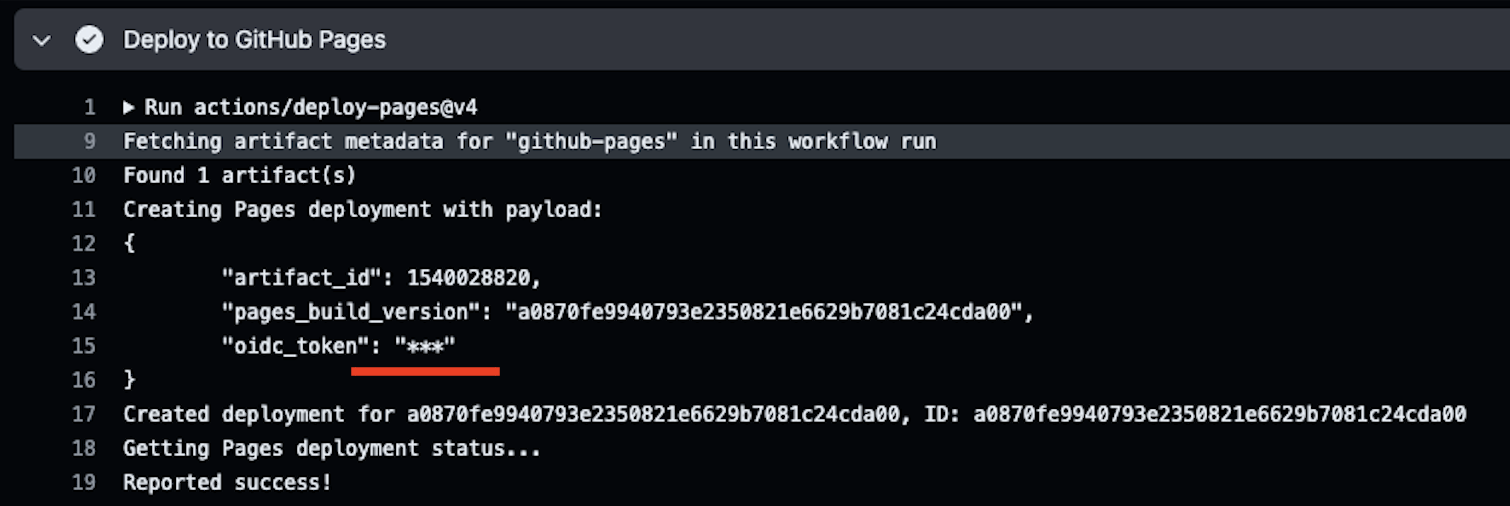
\includegraphics[width=1\linewidth]{actionsLogSecrets.png}
    \caption{Przykład wyświetlania wartości sekretu w logach pipeline}
    \label{fig:enter-label}
\end{figure}

W GitHub Actions sekrety można skonfigurować w ustawieniach repozytorium poprzez następujące kroki:

\begin{enumerate}
\item Przejdź do sekcji "Settings" w swoim repozytorium.
\item Wybierz "Secrets and variables" z menu po lewej stronie.
\item Kliknij "New repository secret", aby dodać nowy sekret.
\end{enumerate}

Po dodaniu, sekrety mogą być używane w plikach YAML definiujących pipeline w następujący sposób:

\begin{lstlisting}[caption=Przykładowa konfiguracja pipeline'u w Github Actions]
- value: ${{ secrets.MY_SECRET }}
\end{lstlisting}

\subsection{Najlepsze praktyki}
Zasady tworzenia efektywnych pipeline'ów CI/CD są zbliżone do zasad tworzenia przejrzystego i czytelnego kodu. Poniżej przedstawiono kluczowe aspekty optymalnego projektowania pipeline'ów.

\subsubsection{Odpowiedzialność}

Każda akcja w pipeline CI/CD powinna realizować zasadę pojedynczej odpowiedzialności, wykonując jedno, dobrze określone zadanie. Unikanie dużych, złożonych plików konfiguracyjnych, które zawierają wszystkie etapy procesu, jest kluczowe dla zachowania przejrzystości oraz łatwości zarządzania pipeline’em. Takie podejście umożliwia również równoczesne wykonywanie różnych akcji tam, gdzie jest to możliwe, co zwiększa efektywność i skraca czas realizacji całego pipeline’u.

Zasada pojedynczej odpowiedzialności (Single Responsibility Principle) jest kluczowa w projektowaniu zarówno kodu, jak i pipeline'ów CI/CD. Robert C. Martin w swojej książce "Clean Architecture: A Craftsman's Guide to Software Structure and Design" \cite{cleanArchitecture} podkreśla, że każda klasa czy moduł powinny mieć tylko jeden powód do zmiany, co przekłada się na lepszą czytelność i łatwość utrzymania kodu.

Przykładowo, proces budowania aplikacji może obejmować następujące kroki:

\begin{itemize}
    \item zbudowanie,
    \item przetestowanie,
    \item analiza kodu (np. przy użyciu SonarQube).
\end{itemize}

Jeśli wszystkie te kroki są opisane w jednej akcji, a każda z czynności zajmuje 1 jednostkę czasu, cały pipeline zakończy się po 3 jednostkach czasu.

\begin{figure}[H]
    \centering
    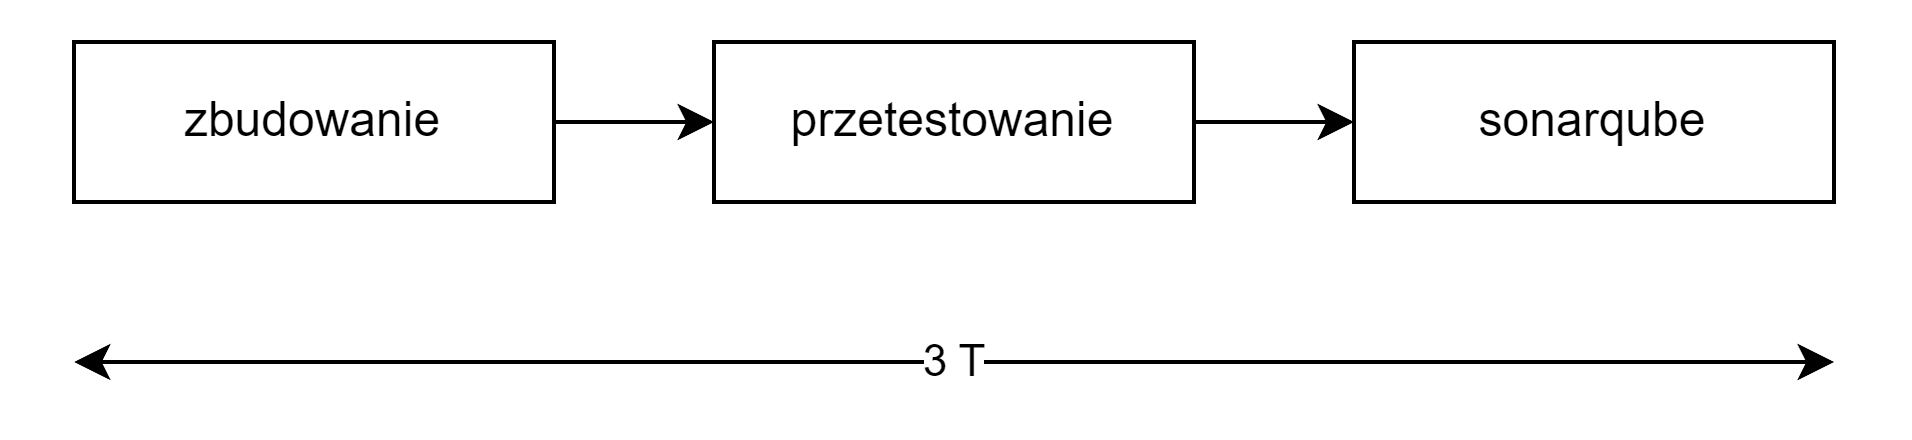
\includegraphics[width=1\linewidth]{pipelines3T.png}
    \caption{Czas trwania nieoptymalnego pipeline}
    \label{fig:enter-label}
\end{figure}

Warto jednak zauważyć, że krok \textbf{budowanie aplikacji} musi być wykonany jako pierwszy, natomiast kroki \textbf{testowanie} oraz \textbf{analiza kodu} mogą być realizowane równolegle, gdyż nie są od siebie zależne. Podział na oddzielne akcje pozwala w takim przypadku skrócić czas wykonania całego pipeline’u do 2 jednostek.

\begin{figure}[H]
    \centering
    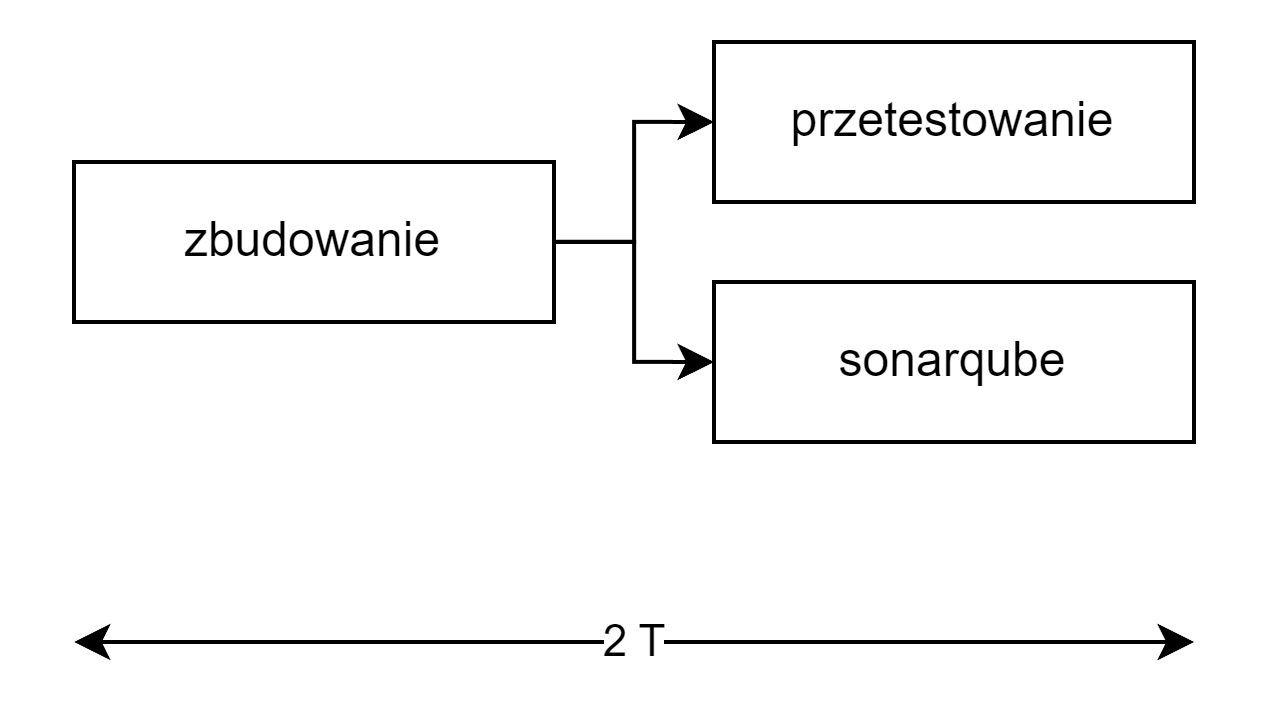
\includegraphics[width=0.5\linewidth]{pipelines2T.png}
    \caption{Czas trwania zoptymalizowanego pipeline}
    \label{fig:enter-label}
\end{figure}

\subsubsection{Abstrakcja}

Efektywnie zaprojektowane akcje powinny być elastyczne i konfigurowalne, umożliwiając ich wykorzystanie w różnych kontekstach, takich jak wdrażanie na środowiska deweloperskie i produkcyjne. Parametryzacja akcji pozwala na ich wielokrotne użycie bez potrzeby modyfikacji kodu każdorazowo.

\begin{figure}[H]
    \centering
    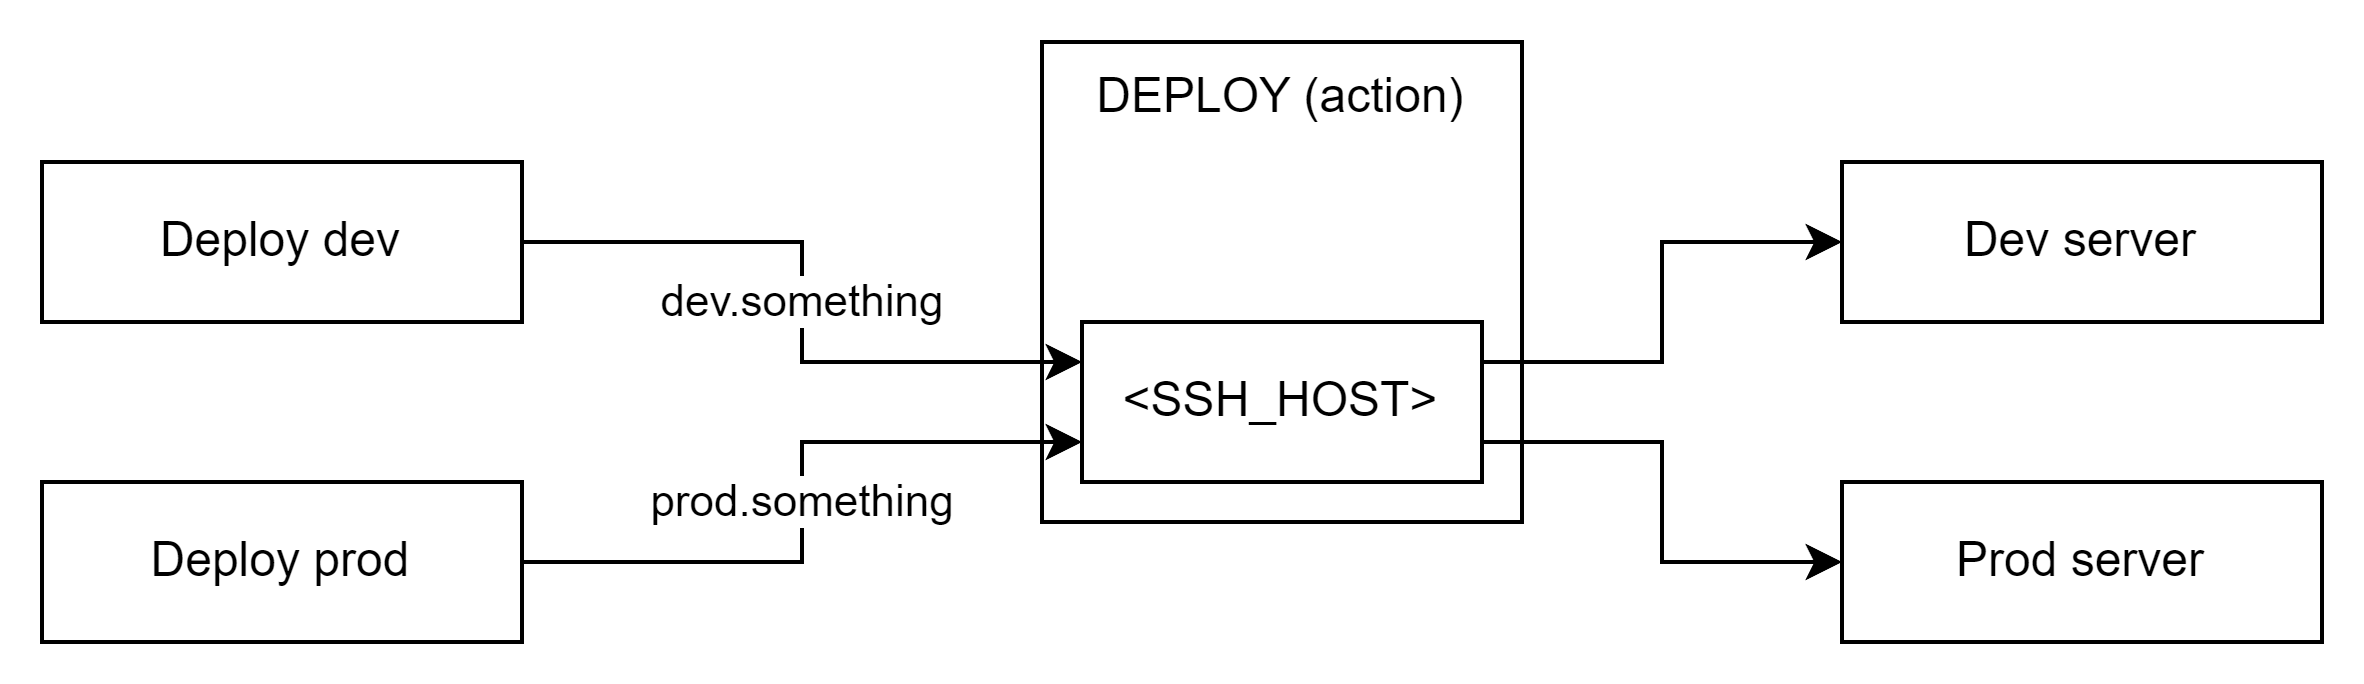
\includegraphics[width=1\linewidth]{pipelinesAbstraction.png}
    \caption{Abstrakcja w pipeline}
    \label{fig:enter-label}
\end{figure}

Dodatkowo, możliwe jest wyniesienie akcji na poziom wyższy niż repozytorium. W przypadku projektu obejmującego kilka mikroserwisów napisanych w tej samej technologii, zasadne może być stworzenie oddzielnego repozytorium dla akcji, w którym zostaną zdefiniowane powtarzalne kroki wspólne dla wszystkich mikroserwisów.

\subsubsection{Idempotencja}

Idempotencja jest kluczowym pojęciem w inżynierii oprogramowania, szczególnie w kontekście systemów rozproszonych i pipeline'ów CI/CD. W artykule "Understanding Idempotency: A Key to Reliable and Scalable Data Pipelines" \cite{understandingIdempotency} opublikowanym na stronie Airbyte, autorzy omawiają znaczenie idempotencji w zapewnianiu spójności i niezawodności w pipeline'ach danych. Podkreślają, że operacje idempotentne mogą być wykonywane wielokrotnie bez zmiany końcowego rezultatu, co jest kluczowe w kontekście powtarzalnych procesów w pipeline'ach CI/CD.

Przykładem akcji nieidempotentnej byłaby akcja budująca obraz Dockerowy, która pobiera repozytorium z głównej gałęzi (main). W takim przypadku rezultat budowy obrazu zależy od bieżącego stanu gałęzi main, co oznacza, że uruchomienie pipeline’u, następnie zmiana na gałęzi main, a ponowne uruchomienie pipeline’u może skutkować budową innego obrazu.

Poprawnym rozwiązaniem w tej sytuacji jest pobranie konkretnego commitu, do którego odniesienie znajduje się w pipeline. Powtórne uruchomienie tego samego pipeline’u zawsze będzie odnosić się do tego samego commitu.

Praktyczne zastosowanie tej zasady może być szczególnie istotne w przypadku potrzeby przywrócenia do poprzedniej, działającej wersji aplikacji. Przykładowo, jeśli wdrożono następujące wersje:
\begin{itemize}
    \item wersja A - wersja funkcjonująca prawidłowo,
    \item wersja B - wersja zawierająca błędy
\end{itemize}

Możliwe jest odnalezienie konkretnego pipeline’u, który wdrażał wersję A, i ponowne jego uruchomienie, co zagwarantuje powrót do działającej wersji aplikacji.

\subsection{Więcej o języku opisu Github Actions}

W dalszej części pracy wykorzystano powtarzalne wzorce stosowane w konfiguracji GitHub Actions. Poniżej przedstawiono podstawowe struktury używane w tworzeniu pipeline’ów.

\subsubsection{Triggery}

Pipeline CI/CD powinien być uruchamiany po wykonaniu określonych akcji związanych z systemem kontroli wersji (Git). GitHub Actions umożliwia definiowanie triggerów, w których można określić warunki uruchomienia pipeline'u. Przykładowo, poniższy fragment kodu konfiguruje pipeline, aby uruchamiał się automatycznie po wykonaniu operacji push na gałęzi main.

\begin{lstlisting}[caption=Fragment kodu z triggerem ustawionym na push na main]
on:
  push:
    branches:
      - main
\end{lstlisting}


\subsubsection{Template}

Najprostszą formą definiowania pipeline’u jest zapis kroków bezpośrednio w pliku \lstinline|.yml|, jednak podejście to nie umożliwia ponownego wykorzystania powtarzalnych fragmentów kodu. Dlatego zalecaną praktyką jest rozdzielenie folderu z pipeline'ami na \lstinline|templates| (szablony) oraz \lstinline|workflows|. Folder \lstinline|templates| zawiera akcje konfigurowalne za pomocą parametrów, natomiast folder \lstinline|workflows| wywołuje te szablony, dostosowując je do konkretnych zastosowań.

\begin{figure}[H]
    \centering
    
\includegraphics[width=0.5\linewidth]{templatesAndWorkflows.png}
    \caption{Diagram przedstawiający w jaki sposób workflows korzystają z szablonów}
    \label{fig:enter-label}
\end{figure}

Poniżej przedstawiono przykładową konfigurację szablonów:

\begin{lstlisting}[caption=Plik \lstinline|.github/templates/templateA/action.yml|]
name: Print message to the screen

inputs:
  message:
    required: true

runs:
  using: "composite"
  steps:
    - name: Print message to the screen
      shell: bash
      run: echo "${{ inputs.message }}"
\end{lstlisting}

\begin{lstlisting}[caption=Plik \lstinline|.github/workflows/workflowA.yml|]
name: Print message to the screen workflow (A)

on:
  push:
    branches:
      - main
jobs:
  main:
    runs-on: ubuntu-latest
    steps:
      - name: Checkout
        uses: actions/checkout@v3
      - name: Invoke print message to the screen
        uses: ./.github/templates/templateA
        with:
          message: "Hello world A!"
\end{lstlisting}

\begin{lstlisting}[caption=Plik \lstinline|.github/workflows/workflowB.yml|]
name: Print message to the screen workflow (B)

on:
  push:
    branches:
      - main
jobs:
  main:
    runs-on: ubuntu-latest
    steps:
      - name: Checkout
        uses: actions/checkout@v3
      - name: Invoke print message to the screen
        uses: ./.github/templates/templateA
        with:
          message: "Hello world B!"
\end{lstlisting}

W efekcie wykonanie akcji push na gałęzi main powoduje uruchomienie dwóch pipeline’ów.

\begin{figure}[H]
    \centering
    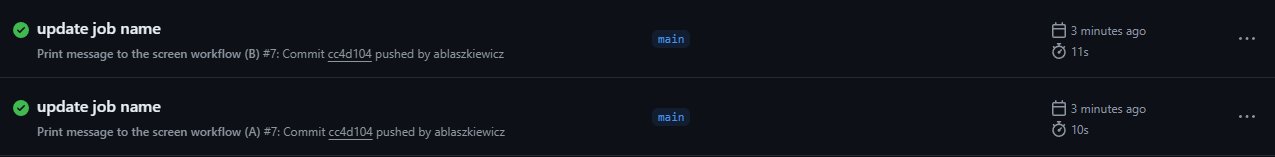
\includegraphics[width=1\linewidth]{testPipelinesInGithubActionsDashboard.png}
    \caption{Wycinek panelu Github actions}
    \label{fig:enter-label}
\end{figure}

Każdy pipeline wyświetla odpowiedni tekst w konsoli:

\begin{figure}[H]
    \centering
    \begin{minipage}[b]{0.45\textwidth}
        \centering
        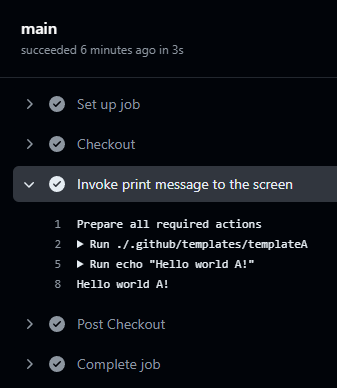
\includegraphics[width=\linewidth]{testPipelinesPipelineA.png}
        \caption{Efekt wykonania pipeline A}
        \label{fig:enter-label-a}
    \end{minipage}
    \hfill
    \begin{minipage}[b]{0.45\textwidth}
        \centering
        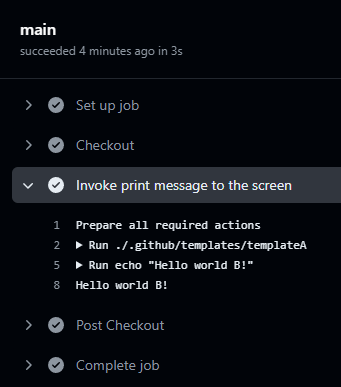
\includegraphics[width=\linewidth]{testPipelinesPipelineB.png}
        \caption{Efekt wykonania pipeline B}
        \label{fig:enter-label-b}
    \end{minipage}
\end{figure}

Szablony są szczególnie użyteczne w przypadku istnienia wielu środowisk. Współczesne standardy DevOps wymagają stosowania wielu środowisk, w tym środowisk testowych, izolowanych od środowisk produkcyjnych, dostępnych często pod adresem \lstinline|https://nazwa-środowiska.oryginalna-domena.pl|. Taka struktura pozwala na testowanie zmian w środowisku zbliżonym do rzeczywistego, minimalizując ryzyko wpływu na środowisko produkcyjne.

\section{Konfiguracja infrastruktury}

\subsection{Serwer}

Rolę serwera pełni maszyna z Ubuntu 22.04 posiadająca 2GB ramu, 10GB dysku oraz 1 współdzielony rdzeń procesora. Nie jest to indywidualna, fizyczna maszyna, a kontener Proxmox. Rozwiązanie to zostało wybrane z uwagi na budżetową naturę - zachowuje się jednak tak samo jak typowo wybierane korporacyjne rozwiązania.

\subsection{Uwierzytelnienie do serwera}

Jak podano w artykule Krakweb \cite{Krakweb}, w procesie uwierzytelniania dostępu do serwera VPS można wyróżnić dwa podstawowe podejścia: uwierzytelnianie kluczem SSH oraz uwierzytelnianie hasłem. Każde z nich ma swoje zalety i wady, które mogą wpływać na wybór jednej z metod w zależności od specyficznych wymagań oraz założeń dotyczących bezpieczeństwa.

\subsubsection{Uwierzytelnienie hasłem}

Uwierzytelnianie hasłem jest jednym z najczęściej stosowanych sposobów ochrony dostępu do serwera. Polega ono na podaniu przez użytkownika nazwy konta oraz odpowiadającego mu hasła podczas logowania.

\begin{itemize}
    \item \textbf{Zalety:}
    \begin{itemize}
        \item \textit{łatwość użycia} - proces logowania jest intuicyjny i nie wymaga zaawansowanej wiedzy technicznej,
        \item \textit{powszechność} - hasła są szeroko stosowane w różnych systemach i aplikacjach, co sprawia, że użytkownicy są zazwyczaj zaznajomieni z tą formą uwierzytelniania,
        \item \textit{brak konieczności konfiguracji dodatkowego oprogramowania} - nie wymaga instalacji czy konfiguracji dodatkowych narzędzi poza podstawową konfiguracją serwera.
    \end{itemize}
    \item \textbf{Wady:}
    \begin{itemize}
        \item \textit{bezpieczeństwo}: hasła mogą być narażone na ataki brute force, phishing, czy przechwytywanie podczas transmisji. Skuteczne hasło musi być odpowiednio długie i skomplikowane, co z kolei może być problematyczne do zapamiętania,
        \item \textit{zarządzanie} - w przypadku wielu użytkowników lub często zmieniającego się personelu, zarządzanie hasłami może stać się trudne i czasochłonne,
        \item \textit{skłonność do słabych haseł} - użytkownicy często tworzą łatwe do odgadnięcia hasła, co zwiększa ryzyko nieautoryzowanego dostępu.
    \end{itemize}
\end{itemize}

\subsubsection{Uwierzytelnienie kluczem SSH}

Uwierzytelnianie kluczem SSH wykorzystuje parę kluczy kryptograficznych (klucz prywatny i klucz publiczny) do uwierzytelniania użytkownika. Klucz publiczny przechowywany jest na serwerze, a klucz prywatny pozostaje na urządzeniu użytkownika.

\begin{itemize}
    \item \textbf{Zalety:}
    \begin{itemize}
        \item \textit{bezpieczeństwo} - klucze SSH są znacznie trudniejsze do złamania w porównaniu z hasłami. Uwierzytelnianie kluczem prywatnym i publicznym zapewnia wysoki poziom bezpieczeństwa,
        \item \textit{brak konieczności przesyłania klucza prywatnego} - podczas procesu logowania klucz prywatny nigdy nie opuszcza maszyny użytkownika, co eliminuje ryzyko jego przechwycenia,
        \item \textit{automatyzacja i skrypty} - uwierzytelnienie kluczem jest wygodne do użycia w skryptach i automatycznych procesach, gdzie podanie hasła byłoby problematyczne.
    \end{itemize}
    \item \textbf{Wady:}
    \begin{itemize}
        \item \textit{złożoność konfiguracji} - proces generowania kluczy, ich instalacja i zarządzanie mogą być bardziej skomplikowane, zwłaszcza dla mniej doświadczonych użytkowników,
        \item \textit{bezpieczeństwo klucza prywatnego} - klucz prywatny musi być przechowywany w bezpiecznym miejscu. W przypadku jego utraty lub przechwycenia, dostęp do serwera może być zagrożony,
        \item \textit{zarządzanie kluczami} - w dużych organizacjach zarządzanie kluczami może być skomplikowane, szczególnie jeśli użytkownicy często się zmieniają.
    \end{itemize}
\end{itemize}

\subsubsection{Implementacja}

Ze względu na wyższy poziom bezpieczeństwa oraz wygodę automatyzacji, wybrano uwierzytelnianie kluczem SSH. Poniżej przedstawiono kroki jego implementacji.

Po zakupie serwera dostarczane są dane logowania, w tym hasło, umożliwiające pierwsze logowanie do serwera. Po zalogowaniu należy wygenerować parę kluczy SSH na lokalnym urządzeniu.

\begin{lstlisting}[caption=Wygenerowanie pary kluczy na swojej maszynie]
cd ~/.ssh
ssh-keygen -t rsa -b 4096
\end{lstlisting}

Powyższe polecenie tworzy pliki \lstinline|id_rsa| oraz \lstinline|id_rsa.pub|. Należy skopiować zawartość pliku \lstinline|id_rsa.pub| i dodać ją do pliku \lstinline|~/.ssh/authorized_keys| na serwerze.

Dla wygody warto także utworzyć plik konfiguracyjny \lstinline|~/.ssh/config| na lokalnym urządzeniu, który będzie zawierał konfigurację połączenia z serwerem. Wartość \lstinline|IdentityFile| to ścieżka do prywatnego klucza SSH.

\begin{lstlisting}[caption=Przykładowa konfiguracja pliku config na lokalnej maszynie]
Host magisterka
    HostName srv15.mikr.us
    User root
    Port 10104
    IdentityFile ~/.ssh/id_rsa
    IdentitiesOnly yes
    ServerAliveInterval 60
\end{lstlisting}

Po zakończeniu konfiguracji połączenie z serwerem można przetestować, wpisując w terminalu \lstinline|ssh magisterka|. Powyższe polecenie powinno umożliwić nawiązanie połączenia z serwerem.

Opcja \lstinline|ServerAliveInterval| utrzymuje połączenie poprzez wysyłanie pingów co 60 sekund, co zapobiega jego zamykaniu w przypadku braku aktywności.

\subsection{Instalacja potrzebnych narzędzi}

Aby zminimalizować liczbę zależności na serwerze, instalowany będzie jedynie Docker. Instalację można przeprowadzić przy użyciu poniższego skryptu:

\begin{lstlisting}[caption=Skrypt instalujący dockera na maszynie Ubuntu]
curl -fsSL https://get.docker.com -o get-docker.sh
sh get-docker.sh
\end{lstlisting}

Po zakończeniu instalacji należy zweryfikować poprawność instalacji, wykonując polecenie \lstinline|docker ps|. Wynik powinien zawierać tabelę Dockera, wskazującą brak aktywnych kontenerów:

\begin{lstlisting}[caption=Wynik wykonania komendy weryfikującej instalację Dockera]
root@l104:~# docker ps
CONTAINER ID   IMAGE     COMMAND   CREATED   STATUS    PORTS     NAMES
\end{lstlisting}


\subsection{Tunelowanie IPv6}

Ze względu na budżetowy charakter wybranego serwera, nie posiada on indywidualnego adresu IPv4, co jest powszechną praktyką obniżającą koszty. W takiej sytuacji dostawca udostępnia jedynie adres IPv6, który nie jest jednak wspierany przez wszystkie sieci.

Rozwiązaniem tego problemu jest skorzystanie z bezpłatnej usługi \textbf{Cloudflare} \footnote{Cloudflare to platforma internetowa oferująca usługi ochrony, przyspieszania i niezawodności stron internetowych poprzez funkcje takie jak sieć dostarczania treści (CDN), ochrona przed atakami DDoS, zarządzanie DNS oraz optymalizacja wydajności.}, po uprzednim podłączeniu do niej domeny. Cloudflare działa w tym przypadku jako serwer proxy: użytkownik, wchodząc na stronę domeny, łączy się z Cloudflare za pośrednictwem IPv4, a Cloudflare następnie przekierowuje ruch do serwera w trybie IPv6.

\begin{figure}[H]
    \centering
    
\includegraphics[width=1\linewidth]{ipv6diagram.png}
    \caption{Zasada działania tunelowania IPv6 Cloudflare}
    \label{fig:enter-label}
\end{figure}

W celu uzyskania adresu IPv6 należy wykonać na serwerze komendę \lstinline|ifconfig|, która wyświetla listę interfejsów sieciowych serwera. Następnie należy odnaleźć pole \lstinline|inet6| i skopiować widoczny tam adres IPv6.

\begin{figure}[H]
    \centering
    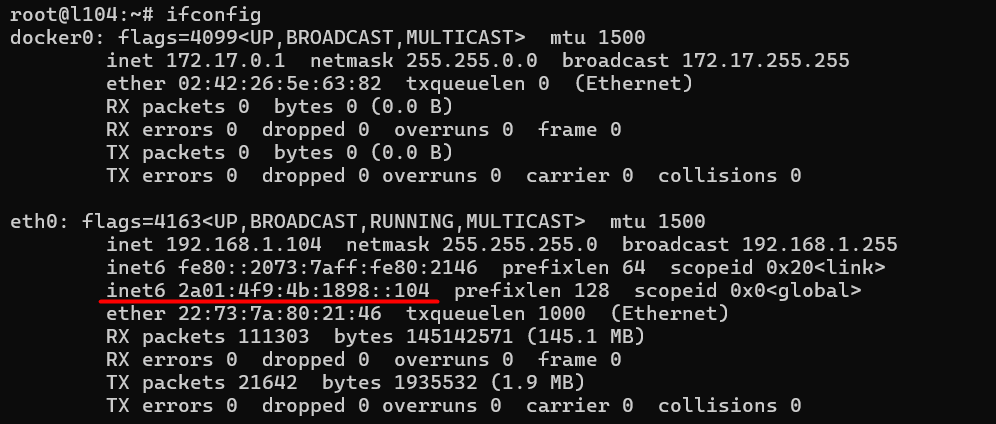
\includegraphics[width=1\linewidth]{ipv6server.png}
    \caption{Lista interfejsów sieciowych serwera z adresem IPv6 serwera zaznaczonym na czerwono}
    \label{fig:enter-label}
\end{figure}

W panelu konfiguracyjnym domeny na platformie Cloudflare, w sekcji \textbf{DNS}, należy dodać rekord typu AAAA, ustawiając nazwę na nazwę domeny, a wartość na wcześniej skopiowany adres IPv6.

\begin{figure}[H]
    \centering
    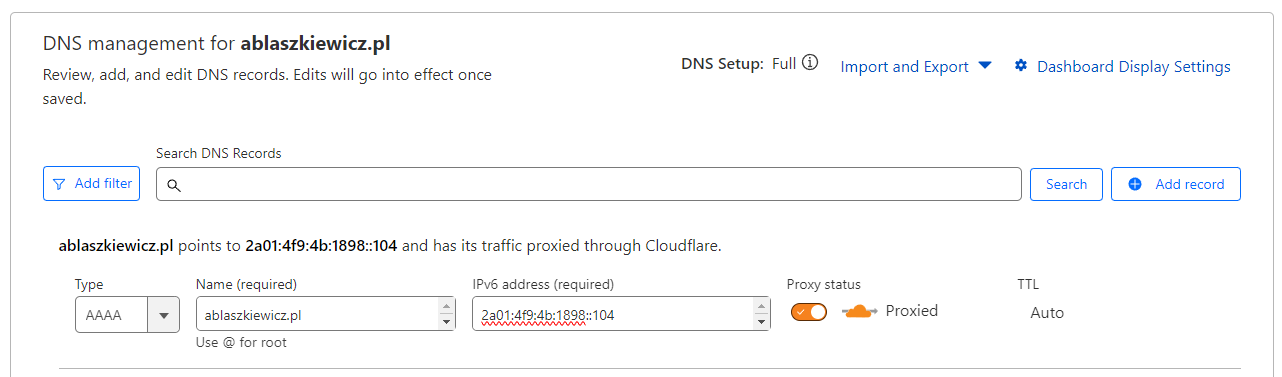
\includegraphics[width=1\linewidth]{ipv6cloudflare.png}
    \caption{Dodanie rekordu AAAA w Cloudflare}
    \label{fig:enter-label}
\end{figure}

Aby sprawdzić poprawność konfiguracji, można uruchomić testowy kontener z obrazem \textbf{nginx} na serwerze, stosując polecenie \lstinline|docker run -p 80:80 nginx|.


Po wykonaniu tych kroków, odwiedzenie strony domeny (w przedstawionym przykładzie ablaszkiewicz.pl) wyświetla stronę powitalną \textbf{nginx}, potwierdzając poprawność konfiguracji.

\begin{figure}[H]
    \centering
    
\includegraphics[width=1\linewidth]{ipv6helloWorld.png}
    \caption{Strona startowa nginx}
    \label{fig:enter-label}
\end{figure}


\section{Reverse proxy}

\subsection{Koncepcja}

W aktualnej konfiguracji dostęp do serwera z poziomu domeny jest ograniczony do jednego serwisu, działającego na porcie 80. Jest to ograniczenie, ponieważ na serwerze planowane jest uruchomienie co najmniej dwóch serwisów — frontendowego i backendowego.

W celu rozwiązania tego problemu stosuje się mechanizm \textbf{reverse proxy}. Zamiast uruchamiać serwis bezpośrednio na porcie 80, na tym porcie konfiguruje się reverse proxy, któremu przypisuje się zestaw reguł kierujących ruch na odpowiednie wewnętrzne porty serwera. Reverse proxy umożliwia nie tylko rozdzielenie ruchu pomiędzy różne serwisy, ale również zapewnia wspólny i niezmienny adres dla usług, co ma kluczowe znaczenie dla dostępności i skalowalności w środowiskach produkcyjnych.

Tradycyjne podejście polega na instalacji narzędzia, takiego jak NGINX, w warstwie systemowej, gdzie dokonuje się jego konfiguracji. Alternatywnym rozwiązaniem, zapewniającym większą elastyczność, jest uruchomienie reverse proxy w kontenerze Docker. Izolacja w kontenerze pozwala na łatwiejsze zarządzanie konfiguracją oraz szybsze przywrócenie poprzednich, działających wersji w przypadku błędów.

\subsection{Implementacja}

Do realizacji mechanizmu reverse proxy zastosowano narzędzie NGINX. Jak podaje oficjalna dokumentacja \cite{NginxDocs}, oprócz funkcji przekierowywania ruchu NGINX może rejestrować logi powiązane z ruchem, co jest użyteczne w analizie i monitorowaniu działania systemu.

Konfiguracja narzędzia została przygotowana tak, aby domyślnie kierować ruch na wewnętrzny port 3000 (przypisany do serwisu frontendowego), podczas gdy żądania zawierające prefiks \lstinline|/api/| będą kierowane na port 3001 (przeznaczony dla backendu).

\begin{figure}[H]
    \centering
    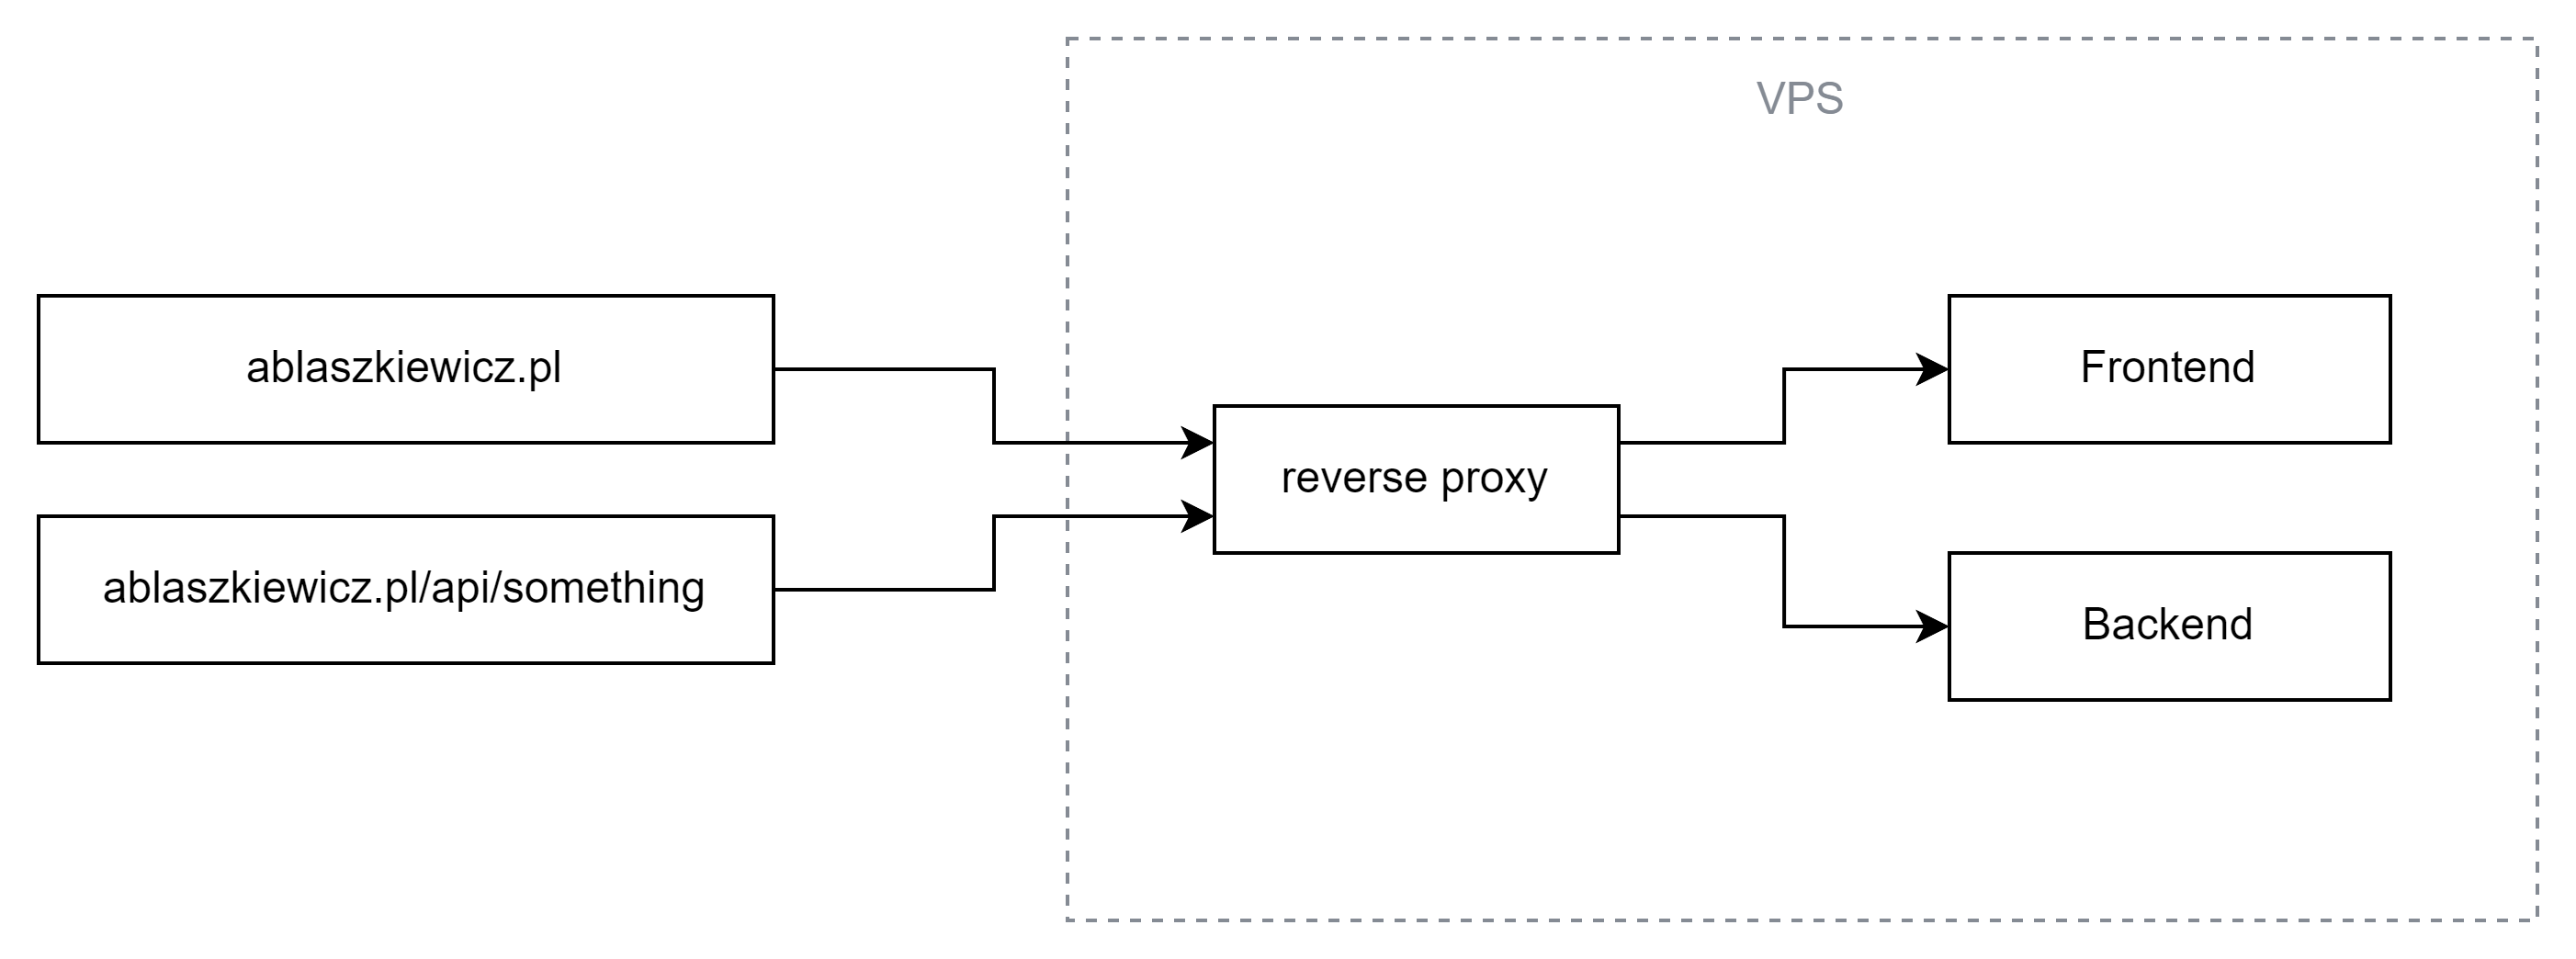
\includegraphics[width=1\linewidth]{reverseProxyDiagram.png}
    \caption{Zasada działania reverse proxy}
    \label{fig:enter-label}
\end{figure}

W celu implementacji reverse proxy przygotowano pliki konfiguracyjne umożliwiające utworzenie obrazu Docker z odpowiednią konfiguracją NGINX.

\begin{lstlisting}[caption=Plik \lstinline|/infrastructure/reverse-proxy/Dockerfile|]
FROM nginx:1.22.0-alpine

WORKDIR /

COPY ./src/nxconf.sh /

RUN chmod +x /nxconf.sh && /nxconf.sh

RUN mkdir -p /var/log/nginx /var/cache/nginx /var/run/nginx && \
    chown -R nginx:nginx /var/log/nginx /var/run/nginx /var/cache/nginx /etc/nginx && \
    sed -e 's#/var/run/nginx.pid#/var/run/nginx/nginx.pid#' -e '/user  nginx;/d'  -i /etc/nginx/nginx.conf

RUN echo "server_names_hash_bucket_size 128;" >/etc/nginx/conf.d/_server_name_hash.conf

RUN echo "client_max_body_size 1g;" >/etc/nginx/conf.d/my_proxy.conf
RUN echo -e "map \$http_upgrade \$connection_upgrade {\n default upgrade;\n '' close;\n}" >/etc/nginx/conf.d/_websocks.conf

EXPOSE 3080

USER nginx

CMD ["nginx", "-g", "daemon off;"]
\end{lstlisting}

\begin{lstlisting}[caption=Plik \lstinline|/infrastructure/reverse-proxy/src/nxconf.sh|]
#!/bin/sh
out="/etc/nginx/conf.d/default.conf"
domain="ablaszkiewicz.pl"
frontend_path="http://192.168.1.104:3000"
backend_path="http://192.168.1.104:3001/"

echo -n > "$out"

config=$(cat <<EOF
server {
    listen       80;
    listen  [::]:80;
    server_name  $domain;

    location = / {
        proxy_pass $frontend_path;
        proxy_set_header Host \$host;
        proxy_http_version 1.1;
        proxy_set_header Upgrade \$http_upgrade;
        proxy_set_header Connection \$connection_upgrade;
        proxy_ssl_name \$host;
        proxy_ssl_server_name on;
        proxy_ssl_verify off;
        proxy_ssl_protocols  TLSv1 TLSv1.1 TLSv1.2;
        proxy_ssl_session_reuse off;
        proxy_set_header X-Forwarded-For \$remote_addr;
        proxy_set_header X-Forwarded-Proto \$scheme;
        proxy_read_timeout 120;
        proxy_send_timeout 120;
        proxy_connect_timeout 120;
    }

    location /api/ {
        proxy_pass $backend_path;
        proxy_set_header Host \$host;
        proxy_http_version 1.1;
        proxy_set_header Upgrade \$http_upgrade;
        proxy_set_header Connection \$connection_upgrade;
        proxy_ssl_name \$host;
        proxy_ssl_server_name on;
        proxy_ssl_verify off;
        proxy_ssl_protocols  TLSv1 TLSv1.1 TLSv1.2;
        proxy_ssl_session_reuse off;
        proxy_set_header X-Forwarded-For \$remote_addr;
        proxy_set_header X-Forwarded-Proto \$scheme;
        proxy_read_timeout 120;
        proxy_send_timeout 120;
        proxy_connect_timeout 120;
    }
}
EOF
)

echo "$config" >> "$out"
\end{lstlisting}

\subsection{Test}

Aby zweryfikować poprawność działania reverse proxy, wykonano na serwerze poniższe komendy:

\begin{lstlisting}[caption=Komendy włączające reverse proxy na serwerze]
git clone https://github.com/ablaszkiewicz/devops-sandbox.git
cd devops-sandbox/infrastructure/reverse-proxy
docker build -t reverse-proxy .
docker run -p 80:80 -d reverse-proxy
docker run -p 3000:80 -d nginx
docker run -p 3001:80 -d httpd
\end{lstlisting}

Po wykonaniu powyższych komend uruchomione zostały następujące serwisy:

\begin{itemize}
    \item port 80 - reverse proxy,
    \item port 3000 - serwis NGINX,
    \item port 3001 - serwis Apache.
\end{itemize}

Połączenie z domeną \lstinline|https://ablaszkiewicz.pl| powinno wyświetlić stronę startową NGINX:

\begin{figure}[H]
    \centering
    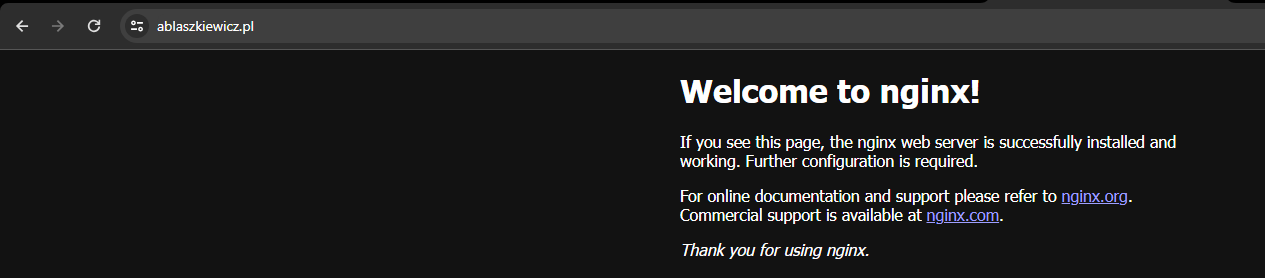
\includegraphics[width=1\linewidth]{reverseProxyNginx.png}
    \caption{Strona startowa nginx}
    \label{fig:enter-label}
\end{figure}

Natomiast przejście do \lstinline|https://ablaszkiewicz.pl/api| powinno przekierować do strony startowej Apache:

\begin{figure}[H]
    \centering
    
\includegraphics[width=1\linewidth]{reverseProxyApache.png}
    \caption{Strona startowa Apache}
    \label{fig:enter-label}
\end{figure}

\subsection{Wiele środowisk}

W optymalnej konfiguracji każde środowisko powinno działać na odrębnej maszynie. W przypadku ograniczeń budżetowych, obydwa środowiska mogą funkcjonować na jednej maszynie, stosując odpowiednie reguły kierowania ruchem. Wcześniej skonfigurowane reverse proxy działa na poziomie lokalizacji w URL (wybierając zasoby na podstawie ścieżki po \lstinline|.pl|), dlatego można je nazwać \textbf{location reverse proxy}. Dla nowych reguł przekierowań, opartych na prefiksie przed nazwą domeny, skonfigurowano \textbf{domain reverse proxy}.

W tej konfiguracji środowisko produkcyjne jest dostępne pod standardową domeną, natomiast środowisko deweloperskie pod prefiksem \lstinline|dev.|.

Nowo skonfigurowane reverse proxy, odpowiedzialne za przekierowania na poziomie domeny, zostało umieszczone przed reverse proxy działającym na poziomie lokalizacji, tworząc następującą strukturę:

\begin{figure}[H]
    \centering
    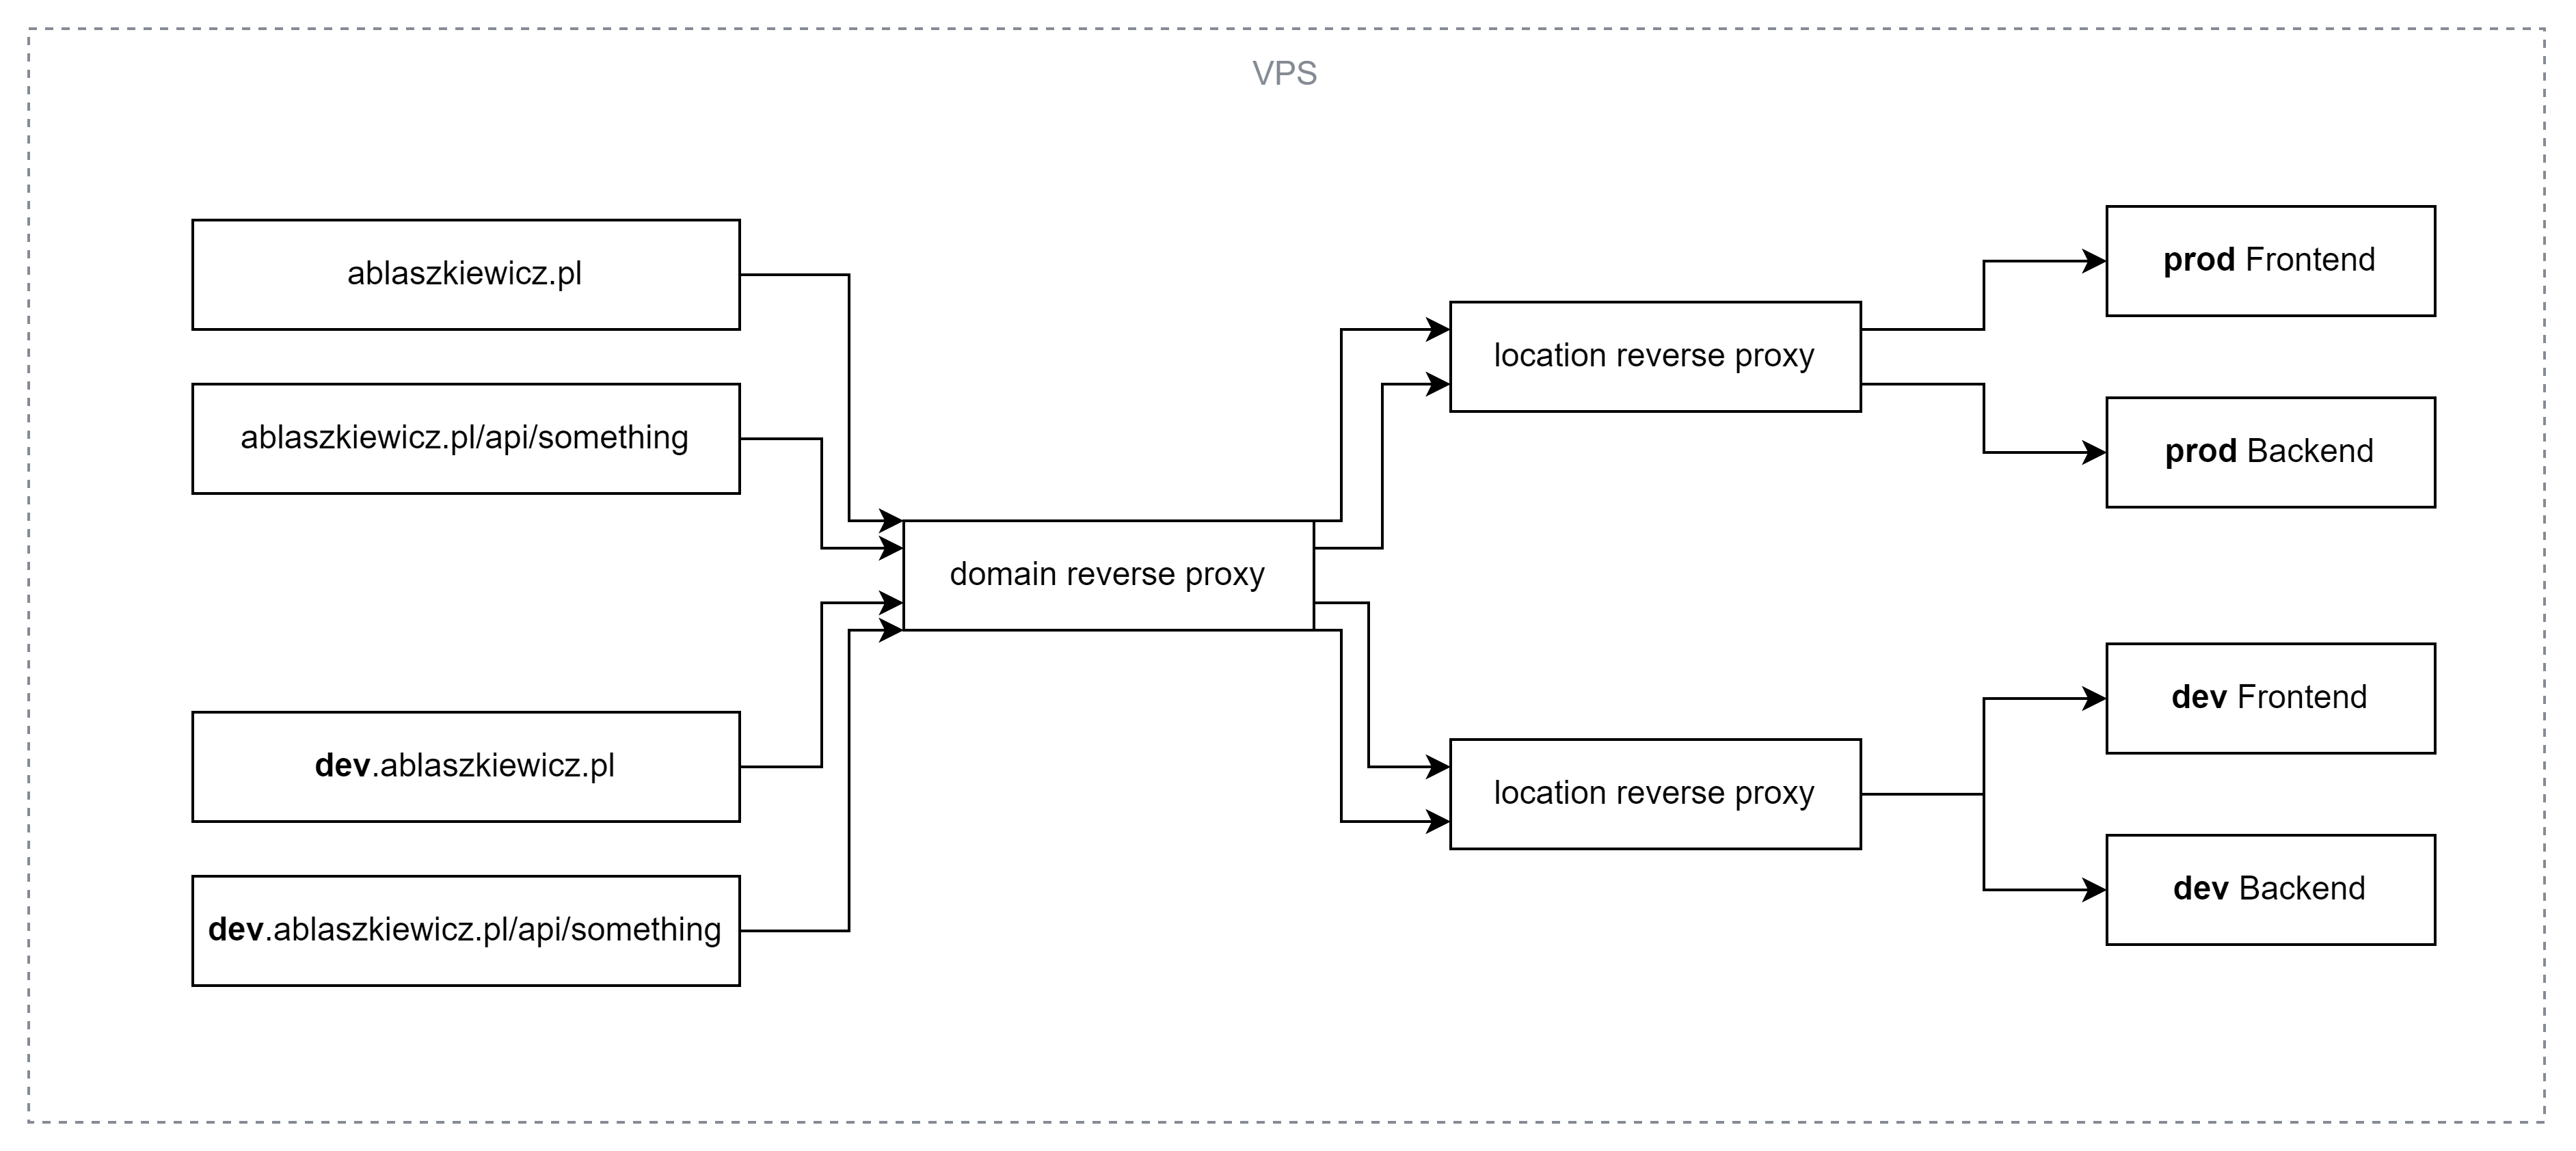
\includegraphics[width=1\linewidth]{domainReverseProxy.png}
    \caption{Diagram przedstawiający zasadę działania reverse proxy przy wielu środowiskach na jednej maszynie}
    \label{fig:enter-label}
\end{figure}

Konfiguracja domain reverse proxy przebiega w sposób analogiczny do poprzednich. Z uwagi na prostotę reguł przekierowań, zastosowano narzędzie \lstinline|proxer| dostępne na platformie GitHub (https://github.com/unkn0w/proxer), które umożliwia zarządzanie przekierowaniami za pomocą prostego pliku konfiguracyjnego i jest dostępne w formie obrazu Docker.

\begin{lstlisting}[caption=Plik \lstinline|/infrastructure/reverse-proxy/src/nxconf.sh|]
my.domain1.com=http://192.168.1.123:3000
my.domain2.com=http://192.168.1.222:8080
my.otherdomain.org=http://somedomain.com
\end{lstlisting}

\subsection{Pipeline}

\subsubsection{Definicja pipeline'u}

Pipeline wdrożeniowy dla komponentu backendowego składa się z następujących etapów:

\begin{itemize}
    \item budowa obrazu Docker,
    \item wypchnięcie obrazu Docker do rejestru,
    \item wdrożenie aplikacji na serwer.
\end{itemize}

\begin{figure}[H]
    \centering
    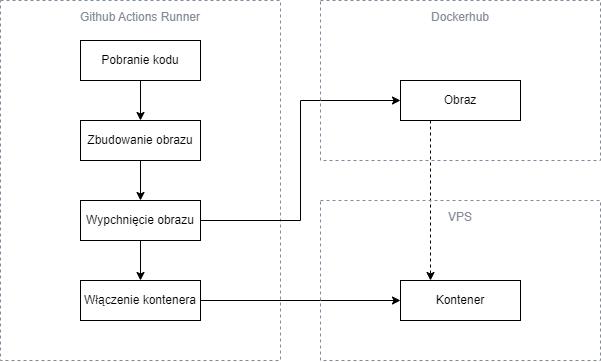
\includegraphics[width=0.75\linewidth]{githubActionsSchema.png}
    \caption{Diagram przedstawiający zasadę działania pipeline do wdrożenia}
    \label{fig:enter-label}
\end{figure}

\subsubsection{Szablon}

Część dotycząca budowy i przesyłania obrazu do rejestru jest uniwersalna i wykorzystywana w różnych przypadkach. W celu standaryzacji przygotowano ogólny szablon \lstinline|.github/templates/build-and-push/action.yml|, który przyjmuje jako parametry dane uwierzytelniające do Docker Hub, kontekst, ścieżkę do pliku \lstinline|Dockerfile| oraz nazwę obrazu. Akcja buduje obraz, a następnie przesyła go do rejestru zgodnie z podanymi parametrami.

Podobnie, wdrożenie kontenera jest procesem, który może być wielokrotnie używany. Szablon \lstinline|.github/templates/deploy-container/action.yml| przyjmuje parametry uwierzytelniające do serwera, nazwę obrazu, nazwę kontenera oraz porty. Akcja loguje się do serwera, uruchamia kontener i przypisuje parametry zgodnie z dostarczonymi danymi.

\begin{figure}[H]
    \centering
    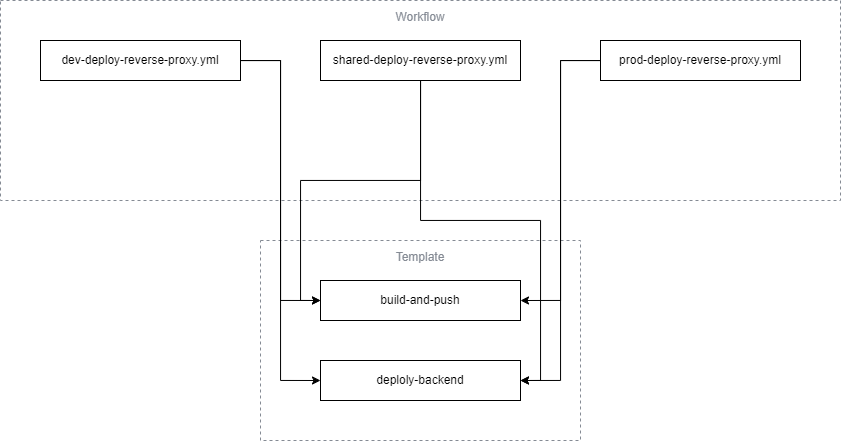
\includegraphics[width=1\linewidth]{reverseProxyTemplatesSchema.png}
    \caption{Diagram przedstawiający użycie template i workflow przy wdrażaniu reverse proxy}
    \label{fig:enter-label}
\end{figure}

\begin{lstlisting}[caption=Plik \texttt{.github/templates/build-and-push/action.yml}]
name: Build and push

inputs:
  # Context
  context:
    required: true
  file:
    required: true

  # Dockerhub
  dockerhub-username:
    required: true
  dockerhub-token:
    required: true
  image-name:
    required: true

runs:
  using: 'composite'
  steps:
    - name: Checkout
      uses: actions/checkout@v3
    - name: Set up QEMU
      uses: docker/setup-qemu-action@v1
    - name: Set up Docker Buildx
      uses: docker/setup-buildx-action@v1
    - name: Login to DockerHub
      uses: docker/login-action@v1
      with:
        username: ${{ inputs.dockerhub-username }}
        password: ${{ inputs.dockerhub-token }}
    - name: Build and push
      id: docker_build
      uses: docker/build-push-action@v2
      with:
        context: ${{ inputs.context }}
        file: ${{ inputs.file }}
        push: true
        tags: ${{ inputs.image-name }}:latest
\end{lstlisting}

\begin{lstlisting}[caption=Plik \texttt{.github/templates/deploy-container/action.yml}]
name: Deploy

inputs:
  # SSH
  host:
    required: true
  username:
    required: true
  port:
    required: true
  ssh-private-key:
    required: true

  # Docker
  image-name:
    required: true
  server-port:
    required: true
  container-name:
    required: true
  application-port:
    required: true

runs:
  using: 'composite'
  steps:
    - name: Update image inside VPS
      uses: appleboy/ssh-action@master
      with:
        host: ${{ inputs.host }}
        USERNAME: ${{ inputs.username }}
        PORT: ${{ inputs.port }}
        KEY: ${{ inputs.ssh-private-key }}
        script: |
          docker rm -f ${{ inputs.container-name }}
          docker pull ${{ inputs.image-name }}
          docker run -d \
          -p ${{ inputs.server-port }}:${{ inputs.application-port }} \
          --restart=always \
          --name ${{ inputs.container-name }} \
          ${{ inputs.image-name }}
\end{lstlisting}

\subsubsection{Workflow}

Szablony pipeline’ów mogą być teraz wykorzystane w trzech plikach workflow, które realizują następujące funkcje:

\begin{itemize}
    \item domain reverse proxy - odpowiedzialne za kierowanie ruchu pomiędzy środowiskami,
    \item 2 location reverse proxy - odpowiedzialne za kierowanie ruchu pomiędzy frontend a backend na konkretnym środowisku.
\end{itemize}

Pliki workflow różnią się głównie nazwą obrazu i portem, na którym kontener zostanie uruchomiony. Założono, że kontenery produkcyjne będą uruchamiane na portach \lstinline|30XX|, a deweloperskie na portach \lstinline|40XX|.

\begin{lstlisting}[caption=Plik \texttt{.github/workflows/dev-deploy-reverse-proxy.yml}]
name: Deploy reverse proxy (dev)

on:
  workflow_dispatch:
  push:
    branches:
      - 'main'

jobs:
  deploy:
    runs-on: ubuntu-latest
    steps:
      - name: Checkout
        uses: actions/checkout@v3
      - name: Build and push
        uses: './.github/templates/build-and-push'
        with:
          context: ./infrastructure/reverse-proxy-dev
          file: ./infrastructure/reverse-proxy-dev/Dockerfile
          dockerhub-username: ${{ secrets.DOCKERHUB_USERNAME }}
          dockerhub-token: ${{ secrets.DOCKERHUB_TOKEN }}
          image-name: ablaszkiewicz/magisterka-reverse-proxy-dev
      - name: Deploy
        uses: './.github/templates/deploy-container'
        with:
          host: ${{ secrets.SSH_HOST }}
          username: ${{ secrets.SSH_USER }}
          port: ${{ secrets.SSH_PORT }}
          ssh-private-key: ${{ secrets.SSH_KEY }}
          server-port: 4080
          application-port: 80
          image-name: ablaszkiewicz/magisterka-reverse-proxy-dev
          container-name: magisterka-reverse-proxy-dev

\end{lstlisting}

\begin{lstlisting}[caption=Plik \texttt{.github/workflows/prod-deploy-reverse-proxy.yml}]
name: Deploy reverse proxy (prod)

on:
  workflow_dispatch:
  push:
    branches:
      - 'main'

jobs:
  deploy:
    runs-on: ubuntu-latest
    steps:
      - name: Checkout
        uses: actions/checkout@v3
      - name: Build and push
        uses: './.github/templates/build-and-push'
        with:
          context: ./infrastructure/reverse-proxy-prod
          file: ./infrastructure/reverse-proxy-prod/Dockerfile
          dockerhub-username: ${{ secrets.DOCKERHUB_USERNAME }}
          dockerhub-token: ${{ secrets.DOCKERHUB_TOKEN }}
          image-name: ablaszkiewicz/magisterka-reverse-proxy-prod
      - name: Deploy
        uses: './.github/templates/deploy-container'
        with:
          host: ${{ secrets.SSH_HOST }}
          username: ${{ secrets.SSH_USER }}
          port: ${{ secrets.SSH_PORT }}
          ssh-private-key: ${{ secrets.SSH_KEY }}
          server-port: 3080
          application-port: 80
          image-name: ablaszkiewicz/magisterka-reverse-proxy-prod
          container-name: magisterka-reverse-proxy-prod

\end{lstlisting}

\begin{lstlisting}[caption=Plik \texttt{.github/workflows/shared-deploy-reverse-proxy.yml}]
name: Deploy reverse proxy (shared)

on:
  workflow_dispatch:
  push:
    branches:
      - 'main'

jobs:
  deploy:
    runs-on: ubuntu-latest
    steps:
      - name: Checkout
        uses: actions/checkout@v3
      - name: Build and push
        uses: './.github/templates/build-and-push'
        with:
          context: ./infrastructure/reverse-proxy-shared
          file: ./infrastructure/reverse-proxy-shared/Dockerfile
          dockerhub-username: ${{ secrets.DOCKERHUB_USERNAME }}
          dockerhub-token: ${{ secrets.DOCKERHUB_TOKEN }}
          image-name: ablaszkiewicz/magisterka-reverse-proxy-shared
      - name: Deploy
        uses: './.github/templates/deploy-container'
        with:
          host: ${{ secrets.SSH_HOST }}
          username: ${{ secrets.SSH_USER }}
          port: ${{ secrets.SSH_PORT }}
          ssh-private-key: ${{ secrets.SSH_KEY }}
          server-port: 80
          application-port: 80
          image-name: ablaszkiewicz/magisterka-reverse-proxy-shared
          container-name: magisterka-reverse-proxy-shared

\end{lstlisting}

\subsection{Porównanie podejść}

\textbf{Kilka serwisów na tym samym porcie}
\begin{itemize}
    \item brak reverse proxy - nie ma możliwości uruchomienia wielu serwisów na tym samym porcie, każdy serwis wymaga oddzielnego portu, co powoduje konieczność używania różnych adresów URL lub portów do ich rozróżnienia,
    \item reverse proxy - umożliwia obsługę wielu serwisów na tym samym porcie poprzez przekierowanie ruchu na różne wewnętrzne porty serwera na podstawie ustalonych reguł,
    \item reverse proxy + docker - działa identycznie jak tradycyjne reverse proxy, z dodatkową zaletą łatwiejszej konfiguracji i izolacji dzięki zastosowaniu kontenerów.
\end{itemize}

\textbf{Bogate logi}
\begin{itemize}
    \item brak reverse proxy - logi są generowane tylko po stronie aplikacji, co ogranicza ich dostępność i możliwości analizy w kontekście całego ruchu sieciowego,
    \item reverse proxy - zapewnia bogate logi, które rejestrują ruch sieciowy, błędy oraz szczegóły dotyczące przekierowań, co pozwala na lepsze monitorowanie i diagnostykę,
    \item reverse proxy + docker - identyczne korzyści jak w przypadku tradycyjnego reverse proxy, z dodatkową możliwością łatwego przechowywania i wersjonowania logów w środowisku kontenerowym.
\end{itemize}

\textbf{Ukrycie wewnętrznych zasad routingu}
\begin{itemize}
    \item brak reverse proxy - nie ma możliwości ukrycia zasad routingu, każdy serwis jest dostępny bezpośrednio z zewnątrz, co ujawnia wewnętrzną strukturę serwera,
    \item reverse proxy - umożliwia ukrycie wewnętrznych zasad routingu poprzez kierowanie ruchu do odpowiednich serwisów w sposób niewidoczny dla użytkowników,
    \item reverse proxy + docker - zapewnia identyczne korzyści jak tradycyjne reverse proxy, ale izolacja kontenerów dodatkowo wzmacnia bezpieczeństwo.
\end{itemize}

\textbf{Banowanie lokalizacji}
\begin{itemize}
    \item brak reverse proxy - możliwość banowania lokalizacji istnieje jedynie po stronie aplikacji, co wymaga dodatkowego kodu lub dedykowanych bibliotek,
    \item reverse proxy - umożliwia łatwe blokowanie dostępu z wybranych lokalizacji, na przykład na podstawie adresu IP czy kraju,
    \item reverse proxy + docker - oferuje te same korzyści co tradycyjne reverse proxy, a dodatkowo umożliwia szybkie wdrożenie zmian dzięki dynamicznej konfiguracji w środowisku kontenerowym.
\end{itemize}

\textbf{Centralne zarządzanie ruchem}
\begin{itemize}
    \item brak reverse proxy - brak centralnego punktu zarządzania ruchem oznacza konieczność ręcznego konfigurowania każdej aplikacji indywidualnie,
    \item reverse proxy - działa jako centralny punkt zarządzania ruchem, umożliwiając łatwe przekierowanie, filtrowanie oraz balansowanie ruchu,
    \item reverse proxy + docker - zapewnia identyczne korzyści jak tradycyjne reverse proxy, a dodatkowo pozwala na łatwą modyfikację konfiguracji dzięki izolacji w kontenerach.
\end{itemize}

\textbf{Odporność na błędy konfiguracji}
\begin{itemize}
    \item brak reverse proxy - nie dotyczy.
    \item reverse proxy - podatne na błędy konfiguracji, które mogą skutkować błędnym przekierowaniem ruchu lub problemami z dostępnością usług,
    \item reverse proxy + docker - zwiększona odporność na błędy dzięki możliwości wersjonowania konfiguracji w plikach i łatwego przywracania poprzednich wersji.
\end{itemize}

\textbf{Wersjonowanie konfiguracji}
\begin{itemize}
    \item brak reverse proxy - nie dotyczy.
    \item reverse proxy - brak natywnego wsparcia dla wersjonowania konfiguracji, co oznacza konieczność ręcznego zarządzania plikami,
    \item reverse proxy + docker - w pełni wspiera wersjonowanie konfiguracji dzięki integracji z systemami kontroli wersji, co pozwala na łatwe śledzenie i cofanie zmian.
\end{itemize}

\textbf{Poziom skomplikowania}
\begin{itemize}
    \item brak reverse proxy - niski poziom skomplikowania dzięki prostocie konfiguracji i ograniczeniu ustawień do podstawowych funkcji serwera,
    \item reverse proxy - średni poziom skomplikowania, wynikający z konieczności konfiguracji dodatkowego narzędzia oraz definicji reguł routingu,
    \item reverse proxy + docker - wysoki poziom skomplikowania, związany z konfiguracją zarówno reverse proxy, jak i środowiska kontenerowego.
\end{itemize}


\begin{table}[H]
\centering
\begin{tabular}{|l|c|c|c|}
\hline
\textbf{Cecha} & \textbf{Brak reverse proxy} & \textbf{Reverse proxy} & \textbf{+docker} \\ \hline
Kilka serwisów na tym samym porcie & \cellcolor{red!50}nie & \cellcolor{green!50}tak & \cellcolor{green!50}tak \\ \hline
Bogate logi  & \cellcolor{yellow!50}po stronie aplikacji & \cellcolor{green!50}tak & \cellcolor{green!50}tak \\ \hline
Ukrycie wewnętrznych zasad routingu & \cellcolor{red!50}nie & \cellcolor{green!50}tak & \cellcolor{green!50}tak \\ \hline
Banowanie lokalizacji & \cellcolor{yellow!50}po stronie aplikacji & \cellcolor{green!50}tak & \cellcolor{green!50}tak \\ \hline
Centralne zarządzanie ruchem & \cellcolor{red!50}nie & \cellcolor{green!50}tak & \cellcolor{green!50}tak \\ \hline
Odporność na błędy konfiguracji & \cellcolor{yellow!50}nie dotyczy & \cellcolor{red!50}nie & \cellcolor{green!50}tak \\ \hline
Wersjonowanie konfiguracji & \cellcolor{yellow!50}nie dotyczy & \cellcolor{red!50}nie & \cellcolor{green!50}tak \\ \hline
Poziom skomplikowanie & \cellcolor{green!50}niski & \cellcolor{yellow!50}średni & \cellcolor{red!50}wysoki \\ \hline
\end{tabular}
\caption{Porównanie podejść z reverse proxy}
\label{tab:porownanie-metod-wdrazania}
\end{table}

\section{Backend}

W tej sekcji omówiono konfigurację pipeline’u dla aplikacji backendowej, wykorzystując wcześniej przygotowane szablony. Proces ten wymaga jedynie zdefiniowania odpowiedniego workflow.


\subsection{Workflow}

Aby uruchomić pipeline, wystarczy wywołać zdefiniowane wcześniej szablony w workflow. 

\begin{lstlisting}[caption=Plik \texttt{.github/workflows/prod-deploy-backend.yml}]
name: Deploy backend (prod)

on:
  workflow_dispatch:
  push:
    branches:
      - main

jobs:
  deploy:
    runs-on: ubuntu-latest
    steps:
      - name: Checkout
        uses: actions/checkout@v3
      - name: Build and push
        uses: './.github/templates/build-and-push'
        with:
          context: ./backend
          file: ./backend/Dockerfile
          dockerhub-username: ${{ secrets.DOCKERHUB_USERNAME }}
          dockerhub-token: ${{ secrets.DOCKERHUB_TOKEN }}
          image-name: ablaszkiewicz/magisterka-backend-prod
      - name: Deploy
        uses: './.github/templates/deploy-container'
        with:
          host: ${{ secrets.SSH_HOST }}
          username: ${{ secrets.SSH_USER }}
          port: ${{ secrets.SSH_PORT }}
          ssh-private-key: ${{ secrets.SSH_KEY }}
          server-port: 3001
          application-port: 3000
          image-name: ablaszkiewicz/magisterka-backend-prod
          container-name: magisterka-backend-prod

\end{lstlisting}

\begin{lstlisting}[caption=Plik \texttt{.github/workflows/dev-deploy-backend.yml}]
name: Deploy backend (dev)

on:
  workflow_dispatch:
  push:
    branches:
      - main

jobs:
  deploy:
    runs-on: ubuntu-latest
    steps:
      - name: Checkout
        uses: actions/checkout@v3
      - name: Build and push
        uses: './.github/templates/build-and-push'
        with:
          context: ./backend
          file: ./backend/Dockerfile
          dockerhub-username: ${{ secrets.DOCKERHUB_USERNAME }}
          dockerhub-token: ${{ secrets.DOCKERHUB_TOKEN }}
          image-name: ablaszkiewicz/magisterka-backend-dev
      - name: Deploy
        uses: './.github/templates/deploy-container'
        with:
          host: ${{ secrets.SSH_HOST }}
          username: ${{ secrets.SSH_USER }}
          port: ${{ secrets.SSH_PORT }}
          ssh-private-key: ${{ secrets.SSH_KEY }}
          server-port: 4001
          application-port: 3000
          image-name: ablaszkiewicz/magisterka-backend-dev
          container-name: magisterka-backend-dev

\end{lstlisting}

Po wysłaniu kodu do GitHub pipeline włącza się automatycznie.

\begin{figure}[H]
    \centering
    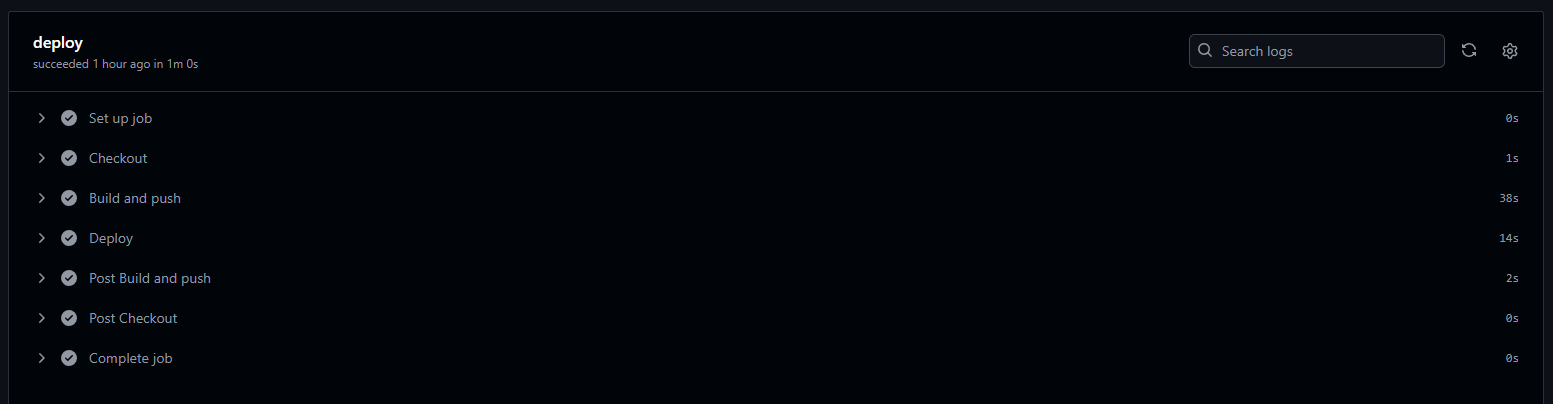
\includegraphics[width=1\linewidth]{pierwszaAkcjaBackendu.png}
    \caption{Rezultat wykonania akcji wdrożenia backendu}
    \label{fig:enter-label}
\end{figure}

Działanie wdrożonej aplikacji można zweryfikować, przechodząc pod adres \lstinline|https://ablaszkiewicz.pl/api/counter|. Poniższy zrzut ekranu potwierdza poprawność działania.

\begin{figure}[H]
    \centering
    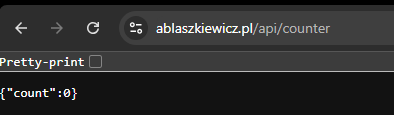
\includegraphics[width=1\linewidth]{rezultatPierwszejWizytyPodBackend.png}
    \caption{Rezultat wejścia na stronę backendu}
    \label{fig:enter-label}
\end{figure}

\subsection{Podsumowanie}

Przeprowadzono eksperyment, w którym poproszono osobę bez wcześniejszego doświadczenia z serwerem i aplikacją o ręczne wdrożenie aplikacji na serwer. Proces ten zajął 7 minut, podczas gdy automatyczne wdrożenie zajmuje 1 minutę.

\begin{figure}[H]
\centering
\begin{tikzpicture}
\begin{axis}[
    ybar,
    bar width=30pt,
    width=0.6\textwidth, % Zmniejszenie szerokości wykresu
    height=8cm,
    symbolic x coords={Ręczne, Automatyczne},
    xtick=data,
    xlabel={Metoda wdrożenia}, % Dodanie opisu osi X
    ylabel={Czas (minuty)},
    ymin=0,
    ymax=8,
    nodes near coords,
    nodes near coords align={vertical},
    title={Porównanie czasu wdrożenia aplikacji},
    enlarge x limits=0.5, % Wyśrodkowanie słupków
]
\addplot coordinates {(Ręczne,7) (Automatyczne,1)};
\end{axis}
\end{tikzpicture}
\caption{Porównanie czasu potrzebnego do ręcznego i automatycznego wdrożenia aplikacji}
\label{fig:czas_wdrozenia}
\end{figure}

Należy zauważyć, że czas trwania automatycznego wdrożenia nie wymaga dodatkowej interakcji ze strony dewelopera, który w tym czasie może realizować inne zadania. W przypadku ręcznego wdrożenia cały czas trwania procesu jest czasem pracy dewelopera.

\begin{table}[H]
\centering
\begin{tabular}{|l|c|c|}
\hline
\textbf{Cecha} & \textbf{Ręczne wdrożenie} & \textbf{Automatyczne wdrożenie} \\ \hline
Konieczność dzielenia sekretów & \cellcolor{red!50}tak & \cellcolor{green!50}nie \\ \hline
Zajmowanie czasu dewelopera & \cellcolor{red!50}tak & \cellcolor{green!50}nie \\ \hline
Odporność na błędy konfiguracji & \cellcolor{red!50}nie & \cellcolor{green!50}tak \\ \hline
Zduplikowanie podejścia dla innych aplikacji & \cellcolor{red!50}nie & \cellcolor{green!50}tak \\ \hline
\end{tabular}
\caption{Porównanie metod wdrożenia}
\label{tab:porownanie-metod-wdrazania}
\end{table}



\section{Frontend}

W tej sekcji omówiono konfigurację pipeline’u dla aplikacji frontendowej z wykorzystaniem wcześniej opracowanych szablonów. W tym celu konieczne jest jedynie zdefiniowanie workflow.

\subsection{Workflow}

Aby uruchomić pipeline, wystarczy odwołać się do wcześniej zdefiniowanych szablonów w workflow.

\begin{lstlisting}[caption=Plik \texttt{.github/workflows/prod-deploy-frontend.yml}]
name: Deploy frontend (prod)

on:
  workflow_dispatch:
  push:
    branches:
      - main

jobs:
  deploy:
    runs-on: ubuntu-latest
    steps:
      - name: Checkout
        uses: actions/checkout@v3
      - name: Build and push
        uses: './.github/templates/build-and-push'
        with:
          context: ./frontend
          file: ./frontend/Dockerfile
          dockerhub-username: ${{ secrets.DOCKERHUB_USERNAME }}
          dockerhub-token: ${{ secrets.DOCKERHUB_TOKEN }}
          image-name: ablaszkiewicz/magisterka-frontend-prod
      - name: Deploy
        uses: './.github/templates/deploy-container'
        with:
          host: ${{ secrets.SSH_HOST }}
          username: ${{ secrets.SSH_USER }}
          port: ${{ secrets.SSH_PORT }}
          ssh-private-key: ${{ secrets.SSH_KEY }}
          server-port: 3000
          application-port: 3000
          image-name: ablaszkiewicz/magisterka-frontend-prod
          container-name: magisterka-frontend-prod

\end{lstlisting}

\begin{lstlisting}[caption=Plik \texttt{.github/workflows/dev-deploy-frontend.yml}]
name: Deploy frontend (dev)

on:
  workflow_dispatch:
  push:
    branches:
      - main

jobs:
  deploy:
    runs-on: ubuntu-latest
    steps:
      - name: Checkout
        uses: actions/checkout@v3
      - name: Build and push
        uses: './.github/templates/build-and-push'
        with:
          context: ./frontend
          file: ./frontend/Dockerfile
          dockerhub-username: ${{ secrets.DOCKERHUB_USERNAME }}
          dockerhub-token: ${{ secrets.DOCKERHUB_TOKEN }}
          image-name: ablaszkiewicz/magisterka-frontend-dev
      - name: Deploy
        uses: './.github/templates/deploy-container'
        with:
          host: ${{ secrets.SSH_HOST }}
          username: ${{ secrets.SSH_USER }}
          port: ${{ secrets.SSH_PORT }}
          ssh-private-key: ${{ secrets.SSH_KEY }}
          server-port: 4000
          application-port: 3000
          image-name: ablaszkiewicz/magisterka-frontend-dev
          container-name: magisterka-frontend-dev

\end{lstlisting}

Po wysłaniu kodu do GitHub akcja włącza się automatycznie.

\begin{figure}[H]
    \centering
    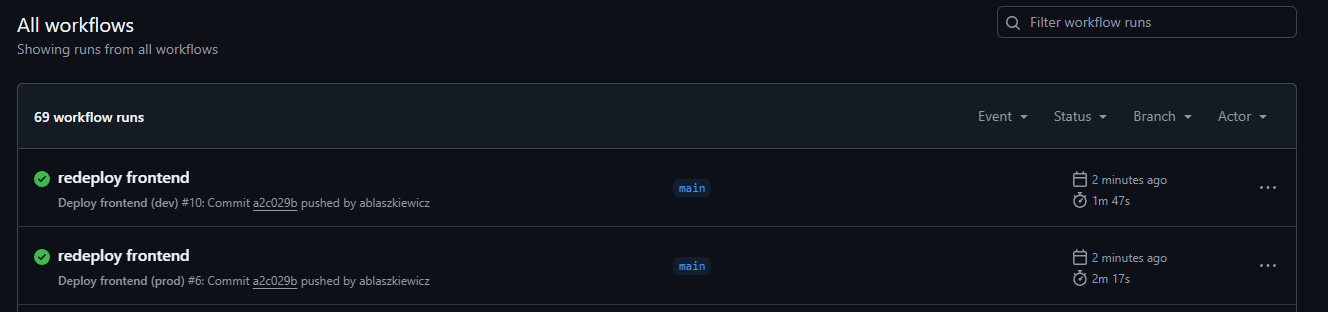
\includegraphics[width=1\linewidth]{rezultatPierwszejAkcjiFrontend.png}
    \caption{Rezultat wdrożenia akcji backendu}
    \label{fig:enter-label}
\end{figure}

Działanie wdrożonej aplikacji można zweryfikować, przechodząc pod adres \lstinline|https://ablaszkiewicz.pl|. Poniższy zrzut ekranu potwierdza poprawność działania aplikacji, w tym funkcjonalność licznika.

\begin{figure}[H]
    \centering
    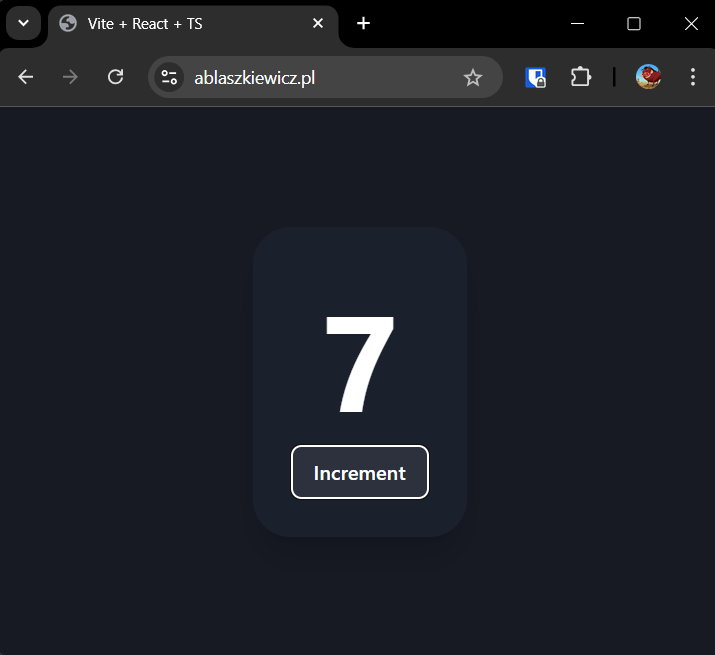
\includegraphics[width=0.5\linewidth]{rezultatWejsciaNaFrontend.png}
    \caption{Rezultat wejścia na stronę frontendu}
    \label{fig:enter-label}
\end{figure}

\section{Podsumowanie dotychczasowej pracy}

W poprzednich sekcjach zostały zrealizowane następujące zadania:

\begin{itemize}
    \item zbadanie podejść budowy aplikacji,
    \item zbadanie podejść budowy obrazów,
    \item zbadanie podejść kierowania ruchem,
    \item konfiguracja infrastruktury,
    \item przygotowanie infrastruktury pod wiele środowisk,
    \item konteneryzacja wszystkich aplikacji oraz elementów infrastruktury,
    \item stworzenie reużywalnych szablonów,
    \item stworzenie workflow do wszystkich aplikacji oraz elementów infrastruktury.
\end{itemize}

Powyższe działania skutkują stworzeniem systemu umożliwiającego automatyczne wdrożenie aplikacji w środowisku produkcyjnym przy każdym wysłaniu kodu na gałąź \lstinline|main| oraz w środowisku deweloperskim przy przesłaniu na gałąź \lstinline|dev|.

\begin{figure}[H]
    \centering
    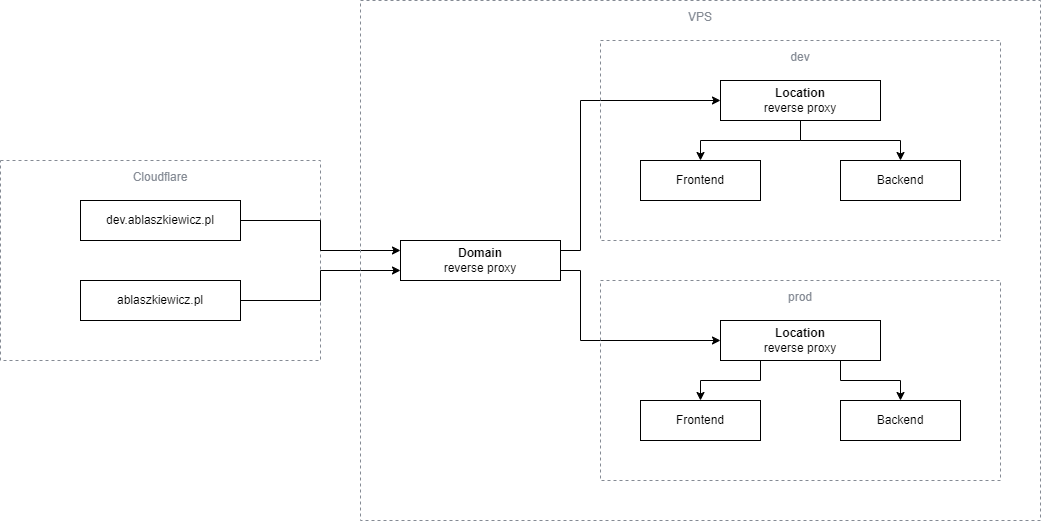
\includegraphics[width=1\linewidth]{diagramInfrasturkturaPolowaPracy.png}
    \caption{Diagram przedstawiający aktualny stan infrastruktury}
    \label{fig:enter-label}
\end{figure}


\section{Observability i monitoring}
\subsection{Cel}

W poprzednich rozdziałach skoncentrowano się na automatyzacji procesów budowania i wdrażania aplikacji, co umożliwiło efektywne wdrożenie kultury DevOps do projektu. Jednak jednym z kluczowych elementów tej kultury jest zapewnienie wysokiego poziomu obserwowalności i monitoringu systemów, co pozwala na utrzymanie stabilności aplikacji oraz szybkie reagowanie na potencjalne problemy.

Celem niniejszego rozdziału jest wprowadzenie rozwiązań, które umożliwią:

\begin{itemize}
    \item \textbf{monitorowanie stanu serwera} — bieżące śledzenie parametrów takich jak wykorzystanie miejsca na dysku, zużycie pamięci RAM oraz obciążenie procesora. Pozwoli to na szybkie wykrywanie anomalii i zapobieganie awariom wynikającym z braku zasobów,
    \item \textbf{zbieranie metryk frontendowych} — uzyskanie informacji na temat interakcji użytkowników z aplikacją, liczby unikalnych odwiedzających, pochodzenia geograficznego oraz czasu ładowania poszczególnych elementów interfejsu,
    \item \textbf{implementację niestandardowych metryk backendowych} — monitorowanie kluczowych aspektów działania aplikacji, takich jak liczba obsłużonych żądań, w celu lepszego zrozumienia wydajności i skalowalności,
    \item \textbf{konfigurację systemu alertów} — automatyczne powiadamianie o krytycznych błędach lub przekroczeniach ustalonych progów zużycia zasobów, co pozwala na szybkie reakcje i minimalizację potencjalnych strat.
\end{itemize}

Nadrzędnym celem jest stworzenie kompleksowego systemu monitoringu, który nie tylko zbiera kluczowe dane, ale także przedstawia je w czytelny i zrozumiały sposób. Dzięki temu możliwe będzie zwiększenie niezawodności i wydajności aplikacji oraz poprawa doświadczeń użytkowników końcowych.

W kolejnych sekcjach przeprowadzony został przegląd dostępnych narzędzi, takich jak Prometheus, Grafana oraz Uptime Kuma, ze wskazaniem ich możliwości, zalet i wad, a następnie opisany zostanie proces implementacji wybranych rozwiązań w kontekście danego projektu.

\subsection{Przegląd narzędzi}

\subsubsection{Narzędzia podstawowe}

Podstawowe narzędzia do monitorowania i \textit{observability} są często wybierane w małych projektach ze względu na swoją prostotę, łatwość wdrożenia oraz niskie koszty. Do najczęściej stosowanych należą:

\begin{itemize}
    \item \textbf{Gatus} – lekki serwer monitorujący, który umożliwia monitorowanie usług poprzez proste konfiguracje w formacie YAML. Oferuje podstawowe powiadomienia i łatwą integrację z istniejącą infrastrukturą. Jest idealny dla prostych zastosowań, gdzie wymagana jest szybka konfiguracja \cite{GatusGithub},

\begin{figure}[H]
    \centering
    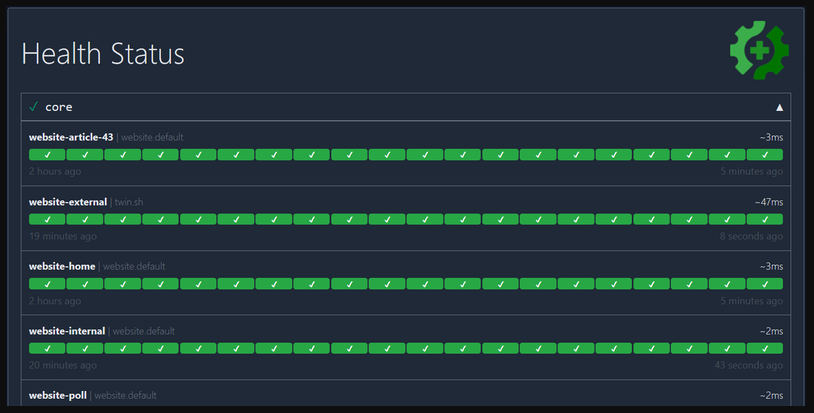
\includegraphics[width=0.5\linewidth]{przykladGatus.png}
    \caption{Przykładowy panel Gatus}
    \label{fig:enter-label}
\end{figure}

    \item \textbf{Uptime Kuma} – przyjazny dla użytkownika monitor serwisów z interfejsem podobnym do Uptime Robot. Pozwala na monitorowanie HTTP(s), TCP, Ping oraz oferuje powiadomienia przez różne kanały, takie jak Telegram czy Slack. Jest łatwy w instalacji i oferuje atrakcyjny interfejs użytkownika \cite{UptimeKumaGithub},

\begin{figure}[H]
    \centering
    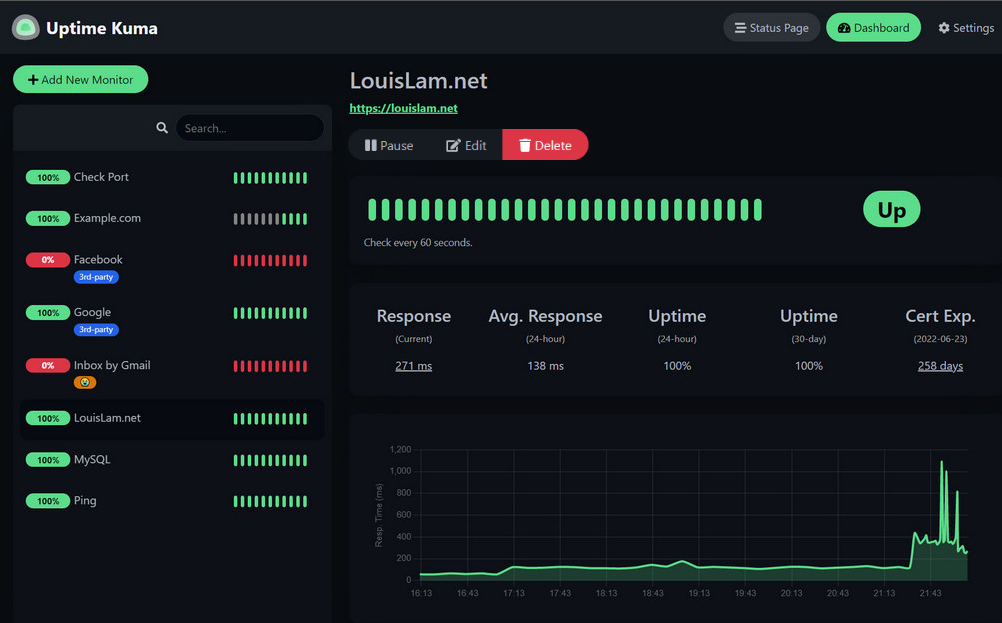
\includegraphics[width=0.5\linewidth]{przykladKuma.png}
    \caption{Przykładowy panel Uptime Kuma}
    \label{fig:enter-label}
\end{figure}

    \item \textbf{Statping} - narzędzie open source do monitorowania statusu usług, które oferuje prosty interfejs i możliwość hostowania własnej strony statusu \cite{StatpingGithub}. Umożliwia monitorowanie usług HTTP(s) i TCP oraz wysyłanie powiadomień. Jest odpowiedni dla małych projektów wymagających podstawowego monitoringu,

\begin{figure}[H]
    \centering
    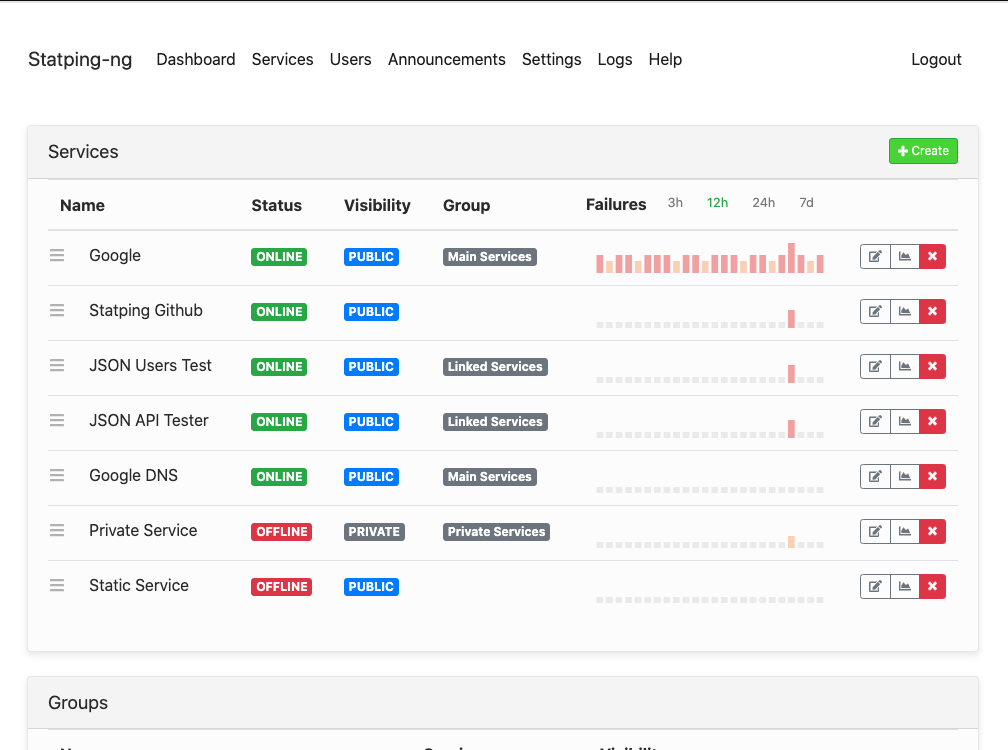
\includegraphics[width=0.5\linewidth]{przykladStatping.png}
    \caption{Przykładowy panel Statping}
    \label{fig:enter-label}
\end{figure}
    
    \item \textbf{Uptime Robot} – popularna usługa SaaS do monitorowania dostępności stron i serwisów. Oferuje darmowy plan z podstawowymi funkcjami oraz płatne plany z dodatkowymi możliwościami i profesjonalnym wsparciem \cite{UptimeRobotMedium}. Dzięki temu jest łatwo dostępny bez konieczności instalacji własnej infrastruktury.

\begin{figure}[H]
    \centering
    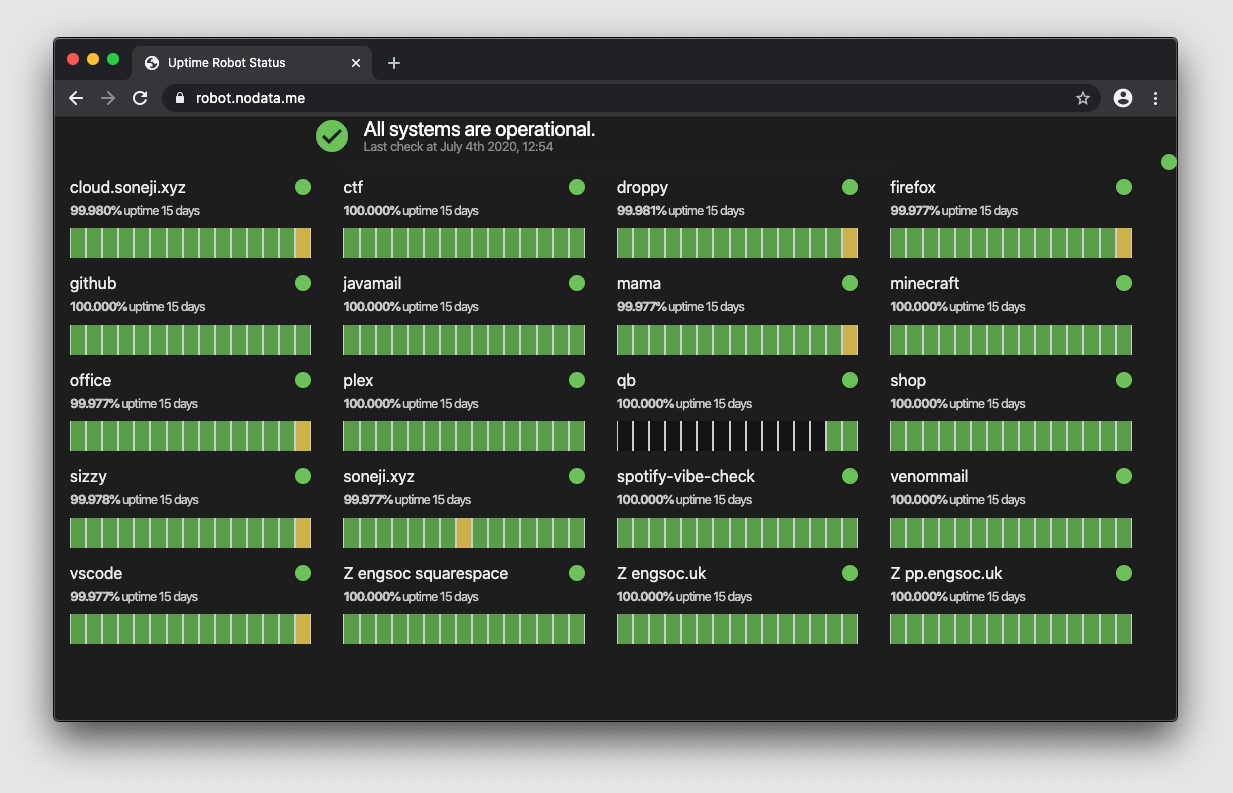
\includegraphics[width=0.5\linewidth]{przykladUptimeRobot.png}
    \caption{Przykładowy panel Uptime Robot}
    \label{fig:enter-label}
\end{figure}
\end{itemize}

\begin{table}[H]
    \centering
    \begin{tabular}{|l|c|c|c|c|}
        \hline
        \textbf{Cecha} & \textbf{Gatus} & \textbf{Uptime Kuma} & \textbf{Statping} & \textbf{Uptime Robot} \\ \hline
        Typ & Open Source & Open Source & Open Source & Usługa SaaS \\ \hline
        Sposób instalacji & Samodzielna & Samodzielna & Samodzielna & Brak instalacji \\ \hline
        Powiadomienia & Tak & Tak & Tak & Tak \\ \hline
        Wspierane protokoły & HTTP, TCP & HTTP(s), TCP, Ping & HTTP(s), TCP & HTTP(s), Ping \\ \hline
        Interfejs użytkownika & Podstawowy & Przyjazny & Podstawowy & Przyjazny \\ \hline
        Skalowalność & Niska & Niska & Niska & Wysoka \\ \hline
        Bezpieczeństwo & Podstawowe & Podstawowe & Podstawowe & Wysokie \\ \hline
        Wsparcie & Społeczność & Społeczność & Społeczność & Profesjonalne \\ \hline
    \end{tabular}
    \caption{Porównanie małych narzędzi monitorujących}
    \label{tab:porownanie-malych-narzedzi}
\end{table}

Podstawowe narzędzia monitorujące, takie jak wymienione powyżej, sprawdzają się w małych projektach, oferując prostotę oraz szybkie wdrożenie przy niskich zasobach. Niemniej jednak w przypadku projektów o większej skali mogą nie spełniać wszystkich wymagań. Z racji tego, że często powstają jako projekty open source tworzone przez niewielkie zespoły, mogą nie oferować optymalnej wydajności ani pełnego bezpieczeństwa, co należy wziąć pod uwagę przy planowaniu długoterminowej strategii monitoringu.


\subsubsection{Prometheus}

Prometheus to otwartoźródłowe narzędzie służące do monitorowania i alertowania, pierwotnie opracowane przez firmę SoundCloud. Obecnie funkcjonuje jako samodzielny projekt open source i jest częścią Fundacji Cloud Native Computing Foundation (CNCF). Narzędzie zostało zaprojektowane z myślą o monitorowaniu dynamicznych środowisk chmurowych.

\begin{figure}[H]
    \centering
    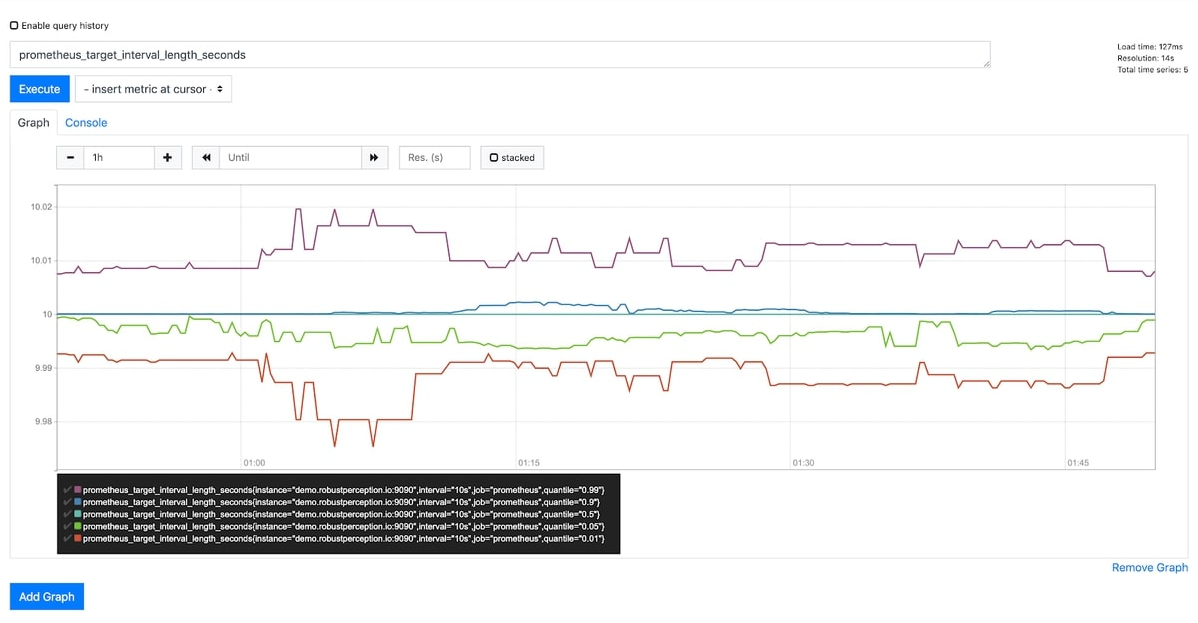
\includegraphics[width=1\linewidth]{prometheusPrzyklad.png}
    \caption{Wynik zapytania o metrykę w panelu Prometheusa}
    \label{fig:enter-label}
\end{figure}

Główne cechy Prometheusa:

\begin{itemize}
    \item \textbf{model danych oparty na szeregach czasowych} — dane są przechowywane jako szeregi czasowe identyfikowane przez nazwę metryki oraz pary klucz-wartość (tzw. \textit{label}),
    \item \textbf{język zapytań PromQL} — elastyczny język zapytań umożliwiający agregację i analizę danych,
    \item \textbf{autonomiczny serwer} — Prometheus nie polega na zewnętrznych systemach przechowywania danych, co zwiększa jego niezawodność,
    \item \textbf{model pull} — dane są pobierane z monitorowanych usług poprzez HTTP, co ułatwia integrację,
    \item \textbf{odkrywanie usług} — wsparcie dla dynamicznego odkrywania usług poprzez integracje z systemami takimi jak Kubernetes czy Consul,
    \item \textbf{alerting} — wbudowany mechanizm alertowania z możliwością integracji z różnymi systemami powiadomień.
\end{itemize}

Prometheus jest idealnym narzędziem dla środowisk \textit{enterprise-grade} ze względu na swoją skalowalność, niezawodność oraz bogaty ekosystem. Pozwala na monitorowanie tysięcy metryk w czasie rzeczywistym, co jest kluczowe w dużych organizacjach. Ponadto, dzięki wsparciu społeczności oraz ciągłemu rozwojowi, Prometheus oferuje aktualne i bezpieczne rozwiązania.

Warto jednak zauważyć, że wdrożenie Prometheusa wymaga pewnej wiedzy i doświadczenia. Konfiguracja może być skomplikowana, a niewłaściwe ustawienia mogą prowadzić do problemów z wydajnością. Dlatego też Prometheus jest często wybierany przez zespoły z odpowiednimi zasobami i kompetencjami technicznymi.

\subsubsection{Grafana}

Grafana to otwartoźródłowa platforma do wizualizacji danych i analizy metryk. Umożliwia tworzenie interaktywnych i dynamicznych dashboardów, które pomagają w monitorowaniu systemów, aplikacji oraz infrastruktury. Grafana integruje się z wieloma źródłami danych, w tym z Prometheusem, Elasticsearch, InfluxDB czy Graphite \cite{BizetyGrafana}.

\begin{figure}[H]
    \centering
    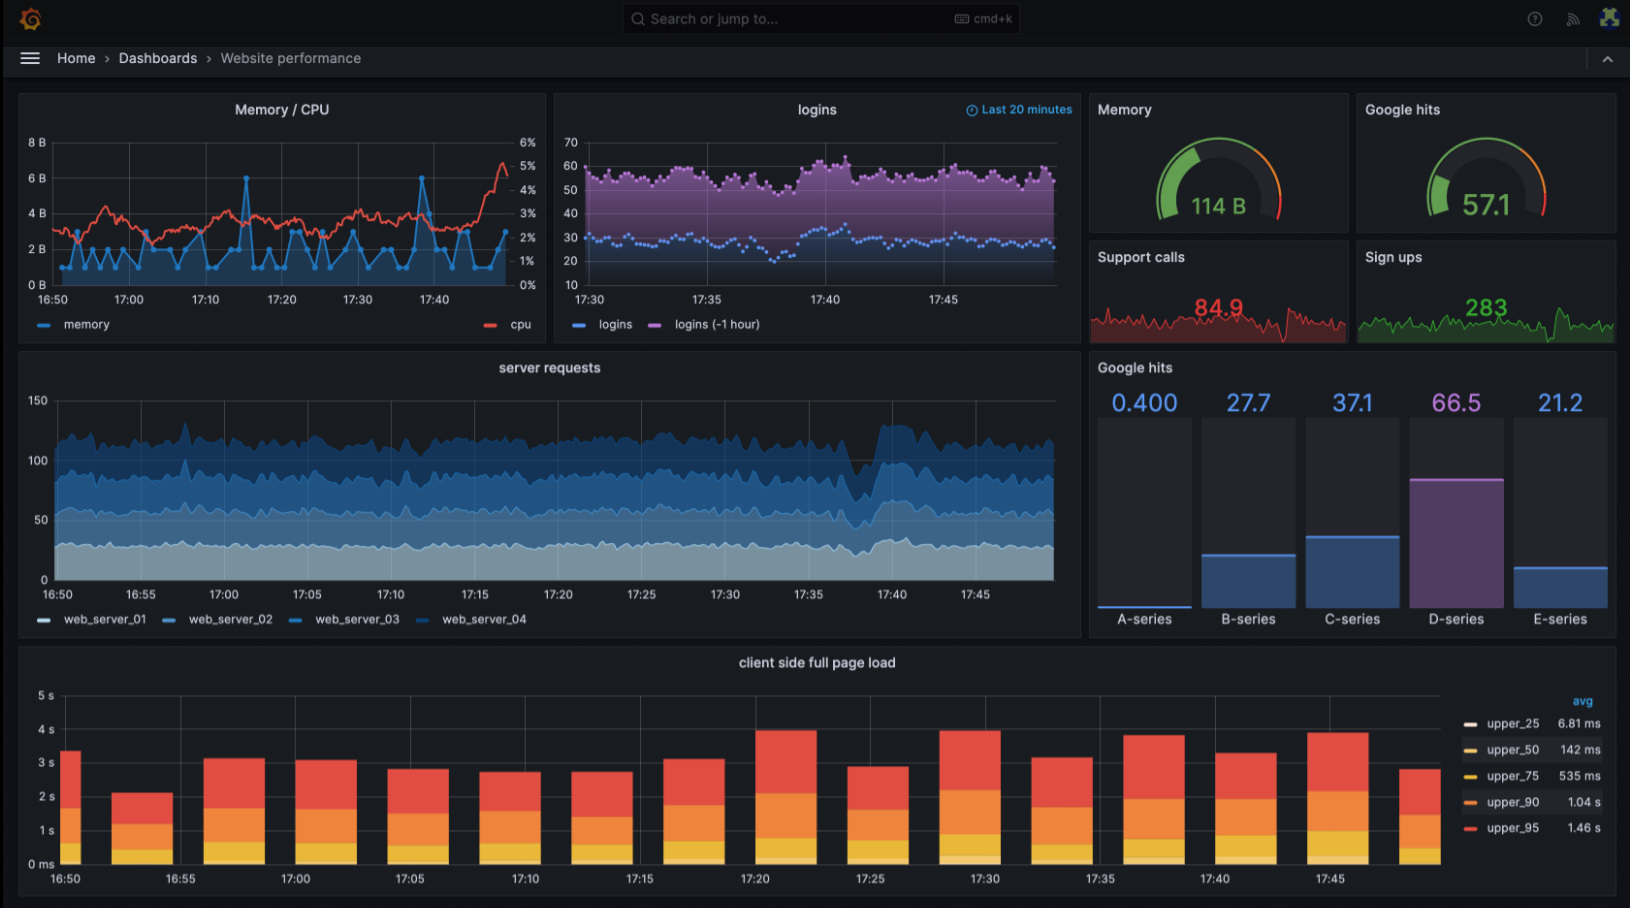
\includegraphics[width=1\linewidth]{grafanaPrzyklad.png}
    \caption{Przykładowy panel w Grafanie}
    \label{fig:enter-label}
\end{figure}

Główne cechy Grafany:

\begin{itemize}
    \item \textbf{Bogate możliwości wizualizacji} — szeroki wybór wykresów, paneli i formatów prezentacji danych,
    \item \textbf{Elastyczność} — możliwość dostosowania dashboardów do indywidualnych potrzeb poprzez edycję paneli i tworzenie własnych wtyczek,
    \item \textbf{Alerting} — wbudowany system alertowania z integracją z różnymi kanałami powiadomień, takimi jak e-mail, Slack czy PagerDuty,
    \item \textbf{Uwierzytelnianie i autoryzacja} — wsparcie dla różnych metod uwierzytelniania, w tym LDAP, OAuth czy Grafana Auth,
    \item \textbf{Społeczność i wsparcie} — aktywna społeczność użytkowników oraz regularne aktualizacje i ulepszenia.
\end{itemize}

Grafana jest często wykorzystywana w środowiskach \textit{enterprise-grade} ze względu na swoją skalowalność i możliwości dostosowania. Umożliwia monitorowanie w czasie rzeczywistym oraz analizę historycznych danych, co jest kluczowe dla dużych organizacji. Ponadto, interaktywne dashboardy ułatwiają zrozumienie złożonych zależności i szybkie reagowanie na problemy.

Podobnie jak w przypadku Prometheusa, wdrożenie Grafany może wymagać zaawansowanej wiedzy technicznej. Konfiguracja źródeł danych, tworzenie zaawansowanych dashboardów czy integracja z systemami alertowania może być skomplikowana dla mniej doświadczonych zespołów.

\subsubsection{VictoriaMetrics}

VictoriaMetrics to wysoko wydajny i skalowalny system przechowywania szeregów czasowych oraz narzędzie monitorujące, które jest kompatybilne z ekosystemem Prometheusa \cite{VictoriaMetricsBlog}. Został stworzony jako odpowiedź na niektóre ograniczenia Prometheusa, szczególnie w kontekście przechowywania długoterminowych danych oraz skalowalności w dużych środowiskach.

\begin{figure}[H]
    \centering
    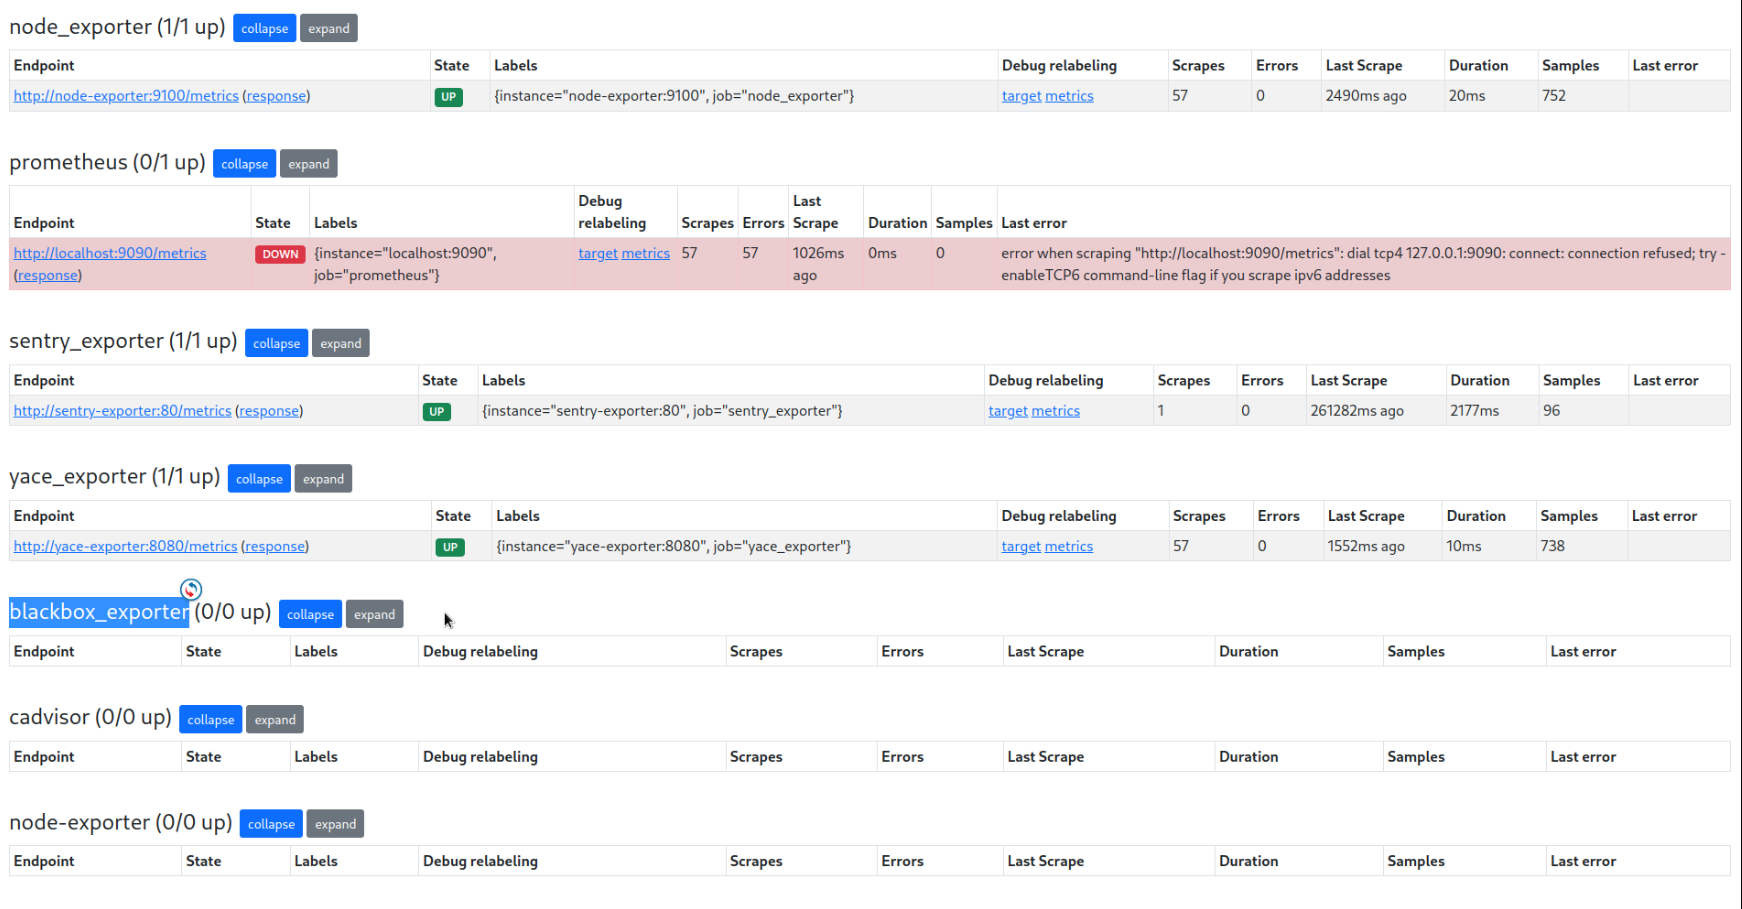
\includegraphics[width=1\linewidth]{victoriaMetricsPrzyklad.png}
    \caption{Przykładowy panel VictoriaMetrics}
    \label{fig:enter-label}
\end{figure}

Główne cechy VictoriaMetrics:

\begin{itemize}
    \item \textbf{Wysoka wydajność i skalowalność} — zaprojektowana do obsługi dużych ilości danych z minimalnym zużyciem zasobów,
    \item \textbf{Kompresja danych} — efektywne algorytmy kompresji, które redukują zużycie przestrzeni dyskowej,
    \item \textbf{Kompatybilność z Prometheusem} — obsługuje protokół zdalnego przechowywania (\textit{Remote Write/Read}), co umożliwia łatwą integrację,
    \item \textbf{Łatwość wdrożenia} — prosty w instalacji i konfiguracji, dostępny jako pojedynczy plik binarny,
    \item \textbf{Wsparcie dla klastrów} — możliwość uruchomienia w trybie klastrowym dla wysokiej dostępności i równoważenia obciążenia.
\end{itemize}

\paragraph{Historia powstania}\mbox{} \\

VictoriaMetrics została stworzona przez zespół inżynierów, którzy zauważyli ograniczenia w istniejących rozwiązaniach do monitorowania i przechowywania danych szeregów czasowych, takich jak Prometheus i InfluxDB. Ich celem było stworzenie narzędzia, które będzie bardziej wydajne pod względem zużycia zasobów oraz lepiej skalowalne w dużych środowiskach.

Pierwsza publiczna wersja VictoriaMetrics została wydana w 2018 roku. Od tego czasu projekt zyskał na popularności wśród firm i organizacji, które potrzebują skalowalnego i wydajnego systemu do monitorowania dużych ilości danych.

\paragraph{Porównanie z Prometheusem}\mbox{} \\


Choć VictoriaMetrics i Prometheus mają wiele wspólnego, istnieją między nimi istotne różnice:

\begin{table}[H]
    \centering
    \begin{tabular}{|l|c|c|}
        \hline
        \textbf{Cecha} & \textbf{Prometheus} & \textbf{VictoriaMetrics} \\ \hline
        Model danych & Szeregi czasowe & Szeregi czasowe \\ \hline
        Skalowalność & Ograniczona & Wysoka \\ \hline
        Długoterminowe przechowywanie & Ograniczone & Efektywne \\ \hline
        Kompresja danych & Podstawowa & Zaawansowana \\ \hline
        Obsługa klastrów & Eksperymentalna & Pełne wsparcie \\ \hline
        Instalacja & Wymaga konfiguracji & Pojedynczy plik binarny \\ \hline
        Ekosystem & Szeroki, duża społeczność & Kompatybilny z Prometheusem \\ \hline
    \end{tabular}
    \caption{Porównanie Prometheusa i VictoriaMetrics}
    \label{tab:porownanie-prometheus-victoriametrics}
\end{table}

\paragraph{Zalety VictoriaMetrics nad Prometheusem:}

\begin{itemize}
    \item \textbf{lepsza skalowalność} — VictoriaMetrics jest w stanie obsłużyć większe obciążenia przy mniejszym zużyciu zasobów,
    \item \textbf{efektywne przechowywanie długoterminowe} — dzięki zaawansowanym algorytmom kompresji, VictoriaMetrics jest bardziej efektywna w przechowywaniu danych historycznych,
    \item \textbf{prostsza instalacja i utrzymanie} — pojedynczy plik binarny ułatwia wdrożenie i zarządzanie,
    \item \textbf{wsparcie dla klastrów} — wbudowane wsparcie dla uruchamiania w trybie klastrowym.
\end{itemize}

\paragraph{Wady w porównaniu z Prometheusem:}

\begin{itemize}
    \item \textbf{mniejsza społeczność} — Prometheus ma większą bazę użytkowników i bardziej rozbudowany ekosystem,
    \item \textbf{mniej wtyczek i integracji} — niektóre narzędzia i wtyczki mogą nie być kompatybilne lub wymagać dodatkowej konfiguracji,
    \item \textbf{mniejsza elastyczność w niektórych obszarach} — niektóre zaawansowane funkcje Prometheusa mogą być trudniejsze do zaimplementowania w VictoriaMetrics.
\end{itemize}


VictoriaMetrics jest odpowiednim wyborem dla organizacji poszukujących skalowalnego systemu monitorowania z długoterminowym przechowywaniem danych. Kompatybilność z Prometheusem ułatwia migrację lub integrację, choć wybór między narzędziami zależy od specyficznych potrzeb organizacji.

\subsubsection{Graphite}
\label{subsubsec:graphite}

\textbf{Graphite} jest kolejnym narzędziem typu \emph{open source}, służącym do przechowywania oraz wizualizacji danych o charakterze szeregów czasowych. Projekt ten powstał pierwotnie w firmie Orbitz w celu monitorowania i analizowania wydajności aplikacji. Dzięki modularnej architekturze, Graphite umożliwia elastyczne gromadzenie metryk z różnych źródeł, oferując przy tym zintegrowany mechanizm wizualizacji danych w postaci wykresów \cite{GraphiteDocs}.

\paragraph{Architektura i główne komponenty.}\mbox{}\\
Podstawowy ekosystem Graphite składa się z trzech kluczowych elementów:
\begin{itemize}
    \item \textbf{Carbon} -- moduł odpowiedzialny za przyjmowanie, parsowanie i zapisywanie przychodzących metryk w bazie danych plików \emph{Whisper},
    \item \textbf{Whisper} -- silnik przechowujący dane szeregów czasowych na dysku w plikach o stałym rozmiarze, stanowiąc alternatywę dla rozwiązań bazodanowych,
    \item \textbf{Graphite Web} -- interfejs webowy, który umożliwia wyświetlanie zgromadzonych danych w postaci wykresów i paneli nawigacyjnych.
\end{itemize}

\paragraph{Funkcjonalności i charakterystyka.}
\begin{itemize}
    \item \textbf{Wielość formatów danych wejściowych} -- Graphite wspiera różne sposoby dostarczania metryk (np.\ protokół \emph{plaintext}, \emph{pickle}) oraz integracje z zewnętrznymi narzędziami.
    \item \textbf{Elastyczna wizualizacja} -- wbudowany interfejs umożliwia tworzenie i dostosowywanie wykresów, a także prostą eksplorację danych historycznych.
    \item \textbf{Skalowanie poziome} -- przy większych wolumenach danych możliwe jest uruchamianie wielu instancji \emph{Carbon} i \emph{Graphite Web} w celu rozłożenia obciążenia.
    \item \textbf{Możliwości analityczne} -- dostępne funkcje transformacji (np.\ \emph{summarize}, \emph{scale}, \emph{movingAverage}) pozwalają na przetwarzanie danych w czasie rzeczywistym.
\end{itemize}

\paragraph{Porównanie z Prometheusem i VictoriaMetrics.}\mbox{}\\
Graphite, w porównaniu z nowocześniejszymi systemami pokroju Prometheus czy VictoriaMetrics, oferuje bardziej tradycyjne podejście oparte na plikach \emph{Whisper} i modelu \emph{push}. Może to być korzystne w niektórych scenariuszach (np.\ tam, gdzie istnieje potrzeba prostego zapisu w lokalnym systemie plików bez rozbudowanej orkiestracji). Z drugiej strony, rozwiązania takie jak Prometheus czy VictoriaMetrics zazwyczaj lepiej sprawdzają się w środowiskach chmurowych oraz oferują wyższą skalowalność i bardziej rozbudowane funkcje analityczne.

\paragraph{Zalety Graphite:}
\begin{itemize}
    \item \textbf{sprawdzona technologia} -- długi okres rozwoju i stabilna społeczność,
    \item \textbf{relatywnie prosty system plików \emph{Whisper}} -- ułatwia samodzielne zarządzanie danymi i rozwiązywanie problemów z zapisem,
    \item \textbf{wbudowany interfejs graficzny} -- umożliwiający przeglądanie metryk bez konieczności integracji z dodatkowymi narzędziami.
\end{itemize}

\paragraph{Wady Graphite:}
\begin{itemize}
    \item \textbf{mniejsza skalowalność} -- w porównaniu z nowocześniejszymi systemami (np.\ Prometheus, VictoriaMetrics) wymaga dodatkowego wysiłku konfiguracyjnego przy dużej liczbie metryk,
    \item \textbf{brak wbudowanego systemu alertowania} -- integracja z zewnętrznymi usługami lub narzędziami (np.\ Grafana Alerting) jest konieczna do realizacji zaawansowanej funkcjonalności alertowania,
    \item \textbf{większy \emph{overhead} przy przechowywaniu danych} -- pliki \emph{Whisper} nie zawsze są optymalne w kontekście długoterminowego przechowywania dużych wolumenów danych.
\end{itemize}

\begin{table}[H]
    \centering
    \begin{tabular}{|l|c|c|c|}
        \hline
        \textbf{Cecha} & \textbf{Graphite} & \textbf{Prometheus} & \textbf{VictoriaMetrics} \\ \hline
        Główny sposób gromadzenia metryk & \emph{Push}         & \emph{Pull}          & \emph{Pull / Push}       \\ \hline
        Mechanizm przechowywania       & Pliki \emph{Whisper} & Wbudowany (TSDB)     & Wbudowany (TSDB)         \\ \hline
        Skalowalność                   & Średnia              & Wysoka               & Bardzo wysoka            \\ \hline
        Alerting                       & Brak wbudowanego      & Wbudowane            & Wbudowane                \\ \hline
        Architektura klastrowa         & Utrudniona           & Eksperymentalna      & Wsparcie pełne           \\ \hline
        Poziom złożoności instalacji   & Średni               & Średni / Wysoki      & Niski / Średni           \\ \hline
    \end{tabular}
    \caption{Porównanie Graphite, Prometheus i VictoriaMetrics}
    \label{tab:porownanie-graphite-prometheus-victoriametrics}
\end{table}

Graphite wciąż pozostaje popularnym rozwiązaniem, szczególnie w środowiskach, gdzie preferuje się klasyczny model \emph{push} lub istnieją już znaczące zasoby oparte na tym systemie. Dla projektów o względnie umiarkowanych potrzebach w zakresie skalowalności i długoterminowego przechowywania danych Graphite może być wystarczający. Jednak w sytuacjach wymagających większej elastyczności i wydajności często rozważa się wdrożenie rozwiązań nowszej generacji, takich jak Prometheus czy VictoriaMetrics.


\subsubsection{Podsumowanie}

Prometheus i Grafana to potężne narzędzia, które w połączeniu oferują kompleksowe rozwiązanie do monitorowania i wizualizacji danych w środowiskach o wysokich wymaganiach. Są one znacznie bardziej zaawansowane niż małe narzędzia omówione wcześniej i pozostają odpowiednim wyborem dla projektów \textit{enterprise-grade}. Z kolei \textbf{Graphite} stanowi alternatywę o dłuższej historii rozwoju, bazującą na modelu \emph{push} i plikach \emph{Whisper}. Mimo że w pewnych zastosowaniach wciąż spełnia swoje zadania (szczególnie przy istniejącej infrastrukturze opartej na tym systemie), w niektórych obszarach może ustępować Prometheusowi pod względem skalowalności, elastyczności oraz wbudowanych funkcji alertowania.

Implementacja i utrzymanie wspomnianych rozwiązań (Prometheus, Grafana oraz Graphite) wymagają jednak większych zasobów oraz wiedzy technicznej. W zamian oferują one skalowalność, wydajność oraz szerokie możliwości dostosowania, co sprawia, że są preferowanym wyborem w dużych organizacjach, gdzie niezawodność, bezpieczeństwo oraz pełna kontrola nad procesem gromadzenia i prezentowania danych stanowią kluczowe elementy infrastruktury.

\subsection{Provisioning}

W dalszej części pracy omówiono proces automatyzacji wdrażania i konfiguracji narzędzi monitorujących, z naciskiem na infrastrukturę. W przypadku monitoringu podejście to jest bardziej złożone i różni się w zależności od używanego narzędzia. Niemniej jednak, twórcy większości rozwiązań monitorujących są świadomi potrzeby automatyzacji, dzięki czemu narzędzia te są odpowiednio przystosowane do takich zastosowań.

Pominięto kroki manualnej instalacji na rzecz wdrażania przy pomocy zautomatyzowanych akcji.

\subsection{Implementacja}

\subsubsection{Uptime Kuma}

Uptime Kuma to lekkie narzędzie do monitorowania dostępności usług i endpointów HTTP. Powstało jako projekt hobbystyczny jednego programisty, który rozpoczął jego rozwój w celu stworzenia alternatywy dla komercyjnych i złożonych systemów monitorowania. Dzięki swojej prostocie i łatwości wdrożenia, szybko zyskało na popularności i przyciągnęło uwagę społeczności open source. Aktualnie projekt ma ponad \textbf{60 000 gwiazdek} na platformie GitHub, co świadczy o jego wysokiej użyteczności oraz aktywnej społeczności deweloperów i użytkowników, która wspólnie rozwija narzędzie \cite{UptimeKumaGithub}.

Główną funkcjonalnością Uptime Kuma jest możliwość monitorowania dostępności usług poprzez regularne wykonywanie żądań HTTP do określonych endpointów. W przypadku wykrycia niedostępności system powiadamia administratora za pomocą skonfigurowanych kanałów, takich jak e-mail, powiadomienia push, integracje z popularnymi komunikatorami, czy webhooki.

W związku z brakiem wsparcia dla automatycznego provisioningu, narzędzie zostało uruchomione za pomocą komendy:

\begin{lstlisting}[caption=Komenda użyta do uruchomienia Uptime Kuma, label=lst:uptime-kuma-run]
docker run -d --restart=unless-stopped -p 8000:3001 -v uptime-kuma:/app/data --name uptime-kuma louislam/uptime-kuma:1
\end{lstlisting}

Po uruchomieniu narzędzia oraz skonfigurowaniu podstawowych danych użytkownika (login i hasło), dodano odpowiedni rekord w ustawieniach domeny, umożliwiając dostęp do narzędzia pod adresem \texttt{status.ablaszkiewicz.pl}. 

Następnie dokonano modyfikacji pliku konfiguracyjnego reverse proxy w celu poprawnego routingu. Zaktualizowany plik konfiguracyjny przedstawiono poniżej:

\begin{lstlisting}[caption=Zmodyfikowany plik konfiguracyjny reverse proxy, label=lst:reverse-proxy-config]
grafana.ablaszkiewicz.pl=http://192.168.1.104:2000
dev.ablaszkiewicz.pl=http://192.168.1.104:4080
ablaszkiewicz.pl=http://192.168.1.104:3080
status.ablaszkiewicz.pl=http://192.168.1.104:8000
\end{lstlisting}

Dodanie monitorów w Uptime Kuma polega na podaniu adresu URL monitorowanego zasobu oraz konfiguracji następujących parametrów:
\begin{itemize}
    \item \textbf{interwał} – czas pomiędzy kolejnymi testami osiągalności serwisu,
    \item \textbf{ponowne próby} – liczba prób przed utworzeniem incydentu po pierwszej nieudanej próbie,
    \item \textbf{akceptowane statusy} – lista statusów HTTP uznawanych za poprawne.
\end{itemize}

Na rysunku \ref{fig:add-monitor} przedstawiono widok interfejsu Uptime Kuma podczas dodawania monitora.

\begin{figure}[H]
    \centering
    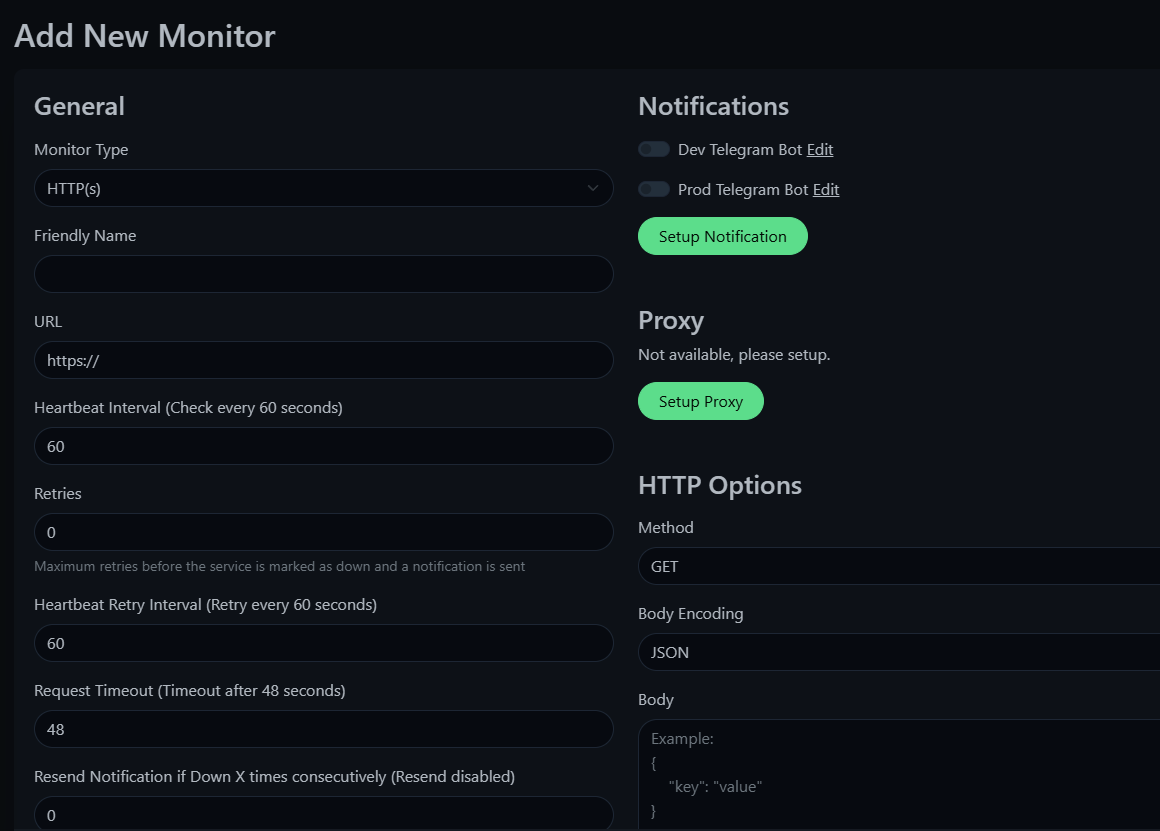
\includegraphics[width=1\linewidth]{uptimeKumaDodawanieMonitora.png}
    \caption{Interfejs dodawania monitora w Uptime Kuma}
    \label{fig:add-monitor}
\end{figure}

Po skonfigurowaniu wszystkich monitorów główny panel aplikacji prezentuje się jak na rysunku \ref{fig:dashboard}.

\begin{figure}[H]
    \centering
    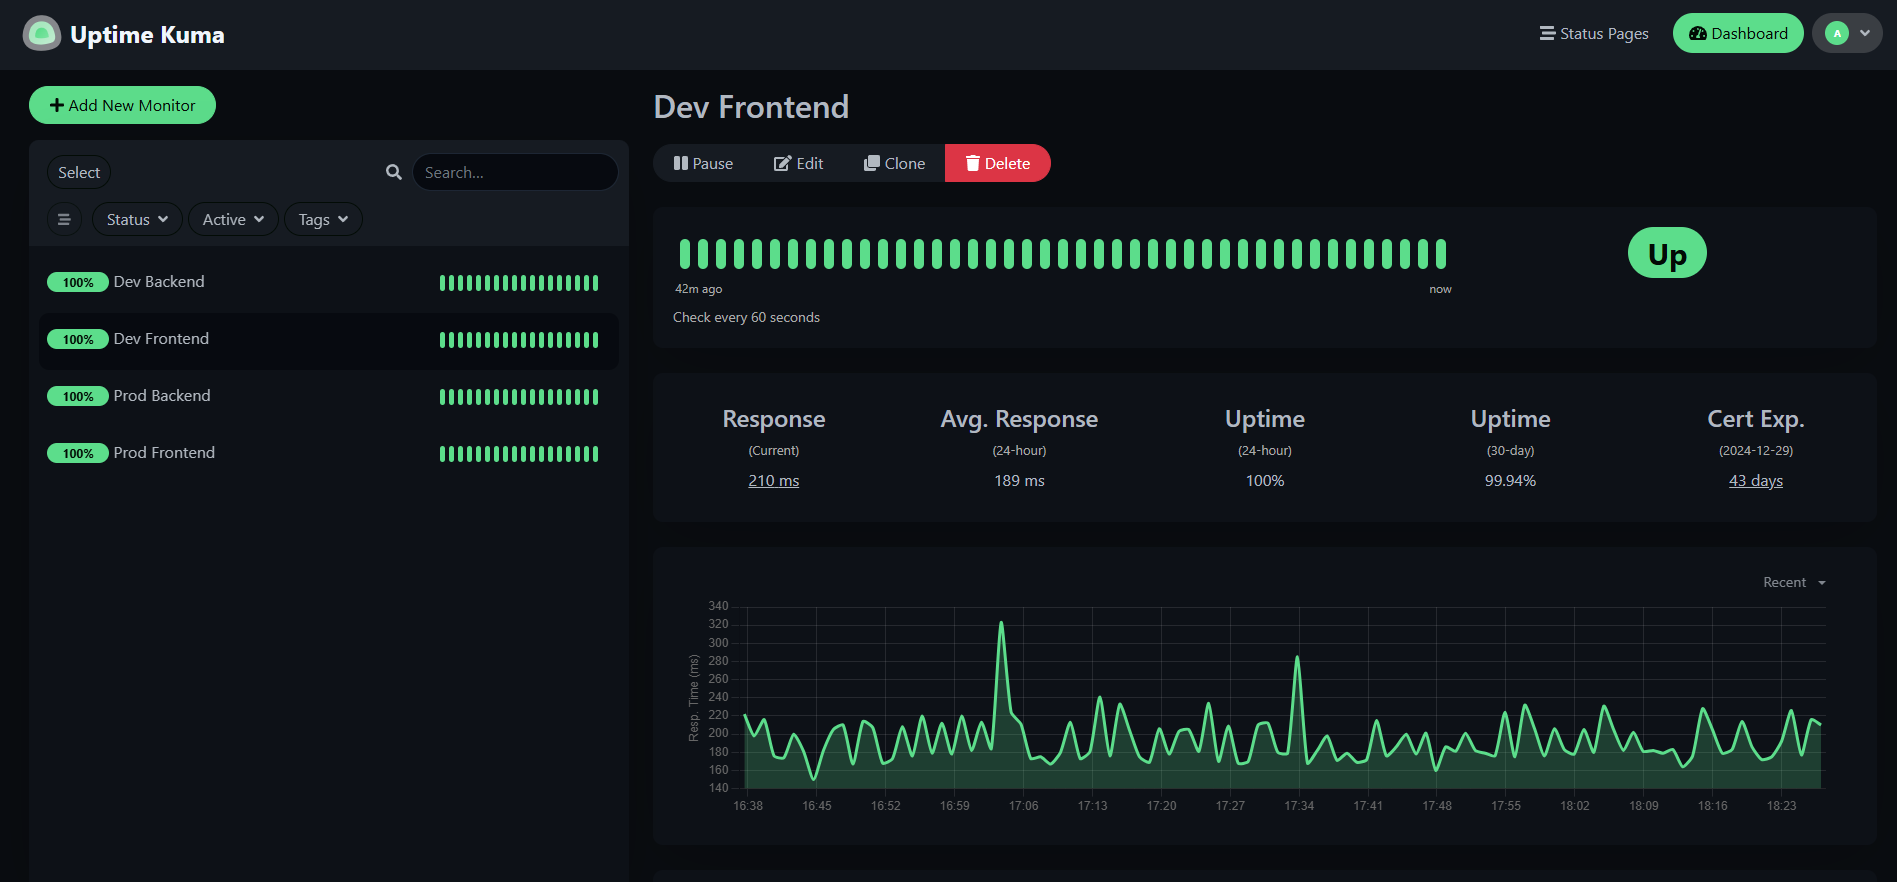
\includegraphics[width=1\linewidth]{uptimeKumaDashboard.png}
    \caption{Główny panel Uptime Kuma}
    \label{fig:dashboard}
\end{figure}


Jedną z istotnych funkcjonalności oferowanych przez Uptime Kuma jest możliwość wysyłania alertów. Po podstawowej konfiguracji bota Telegram, użytkownik otrzymuje powiadomienia o wystąpieniu oraz rozwiązaniu incydentu. Przykład powiadomienia przedstawiono na rysunku \ref{fig:telegram-alert}.

\begin{figure}[H]
    \centering
    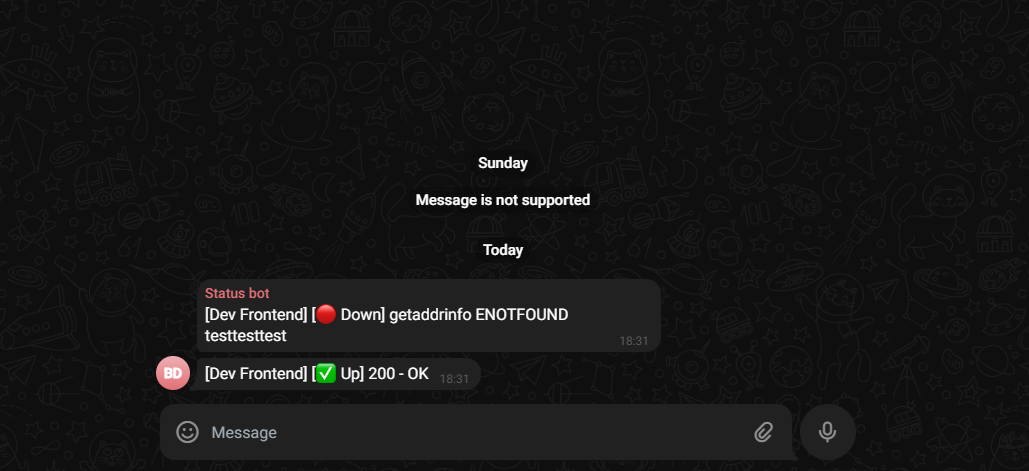
\includegraphics[width=1\linewidth]{uptimeKumaTelegram.png}
    \caption{Przykład powiadomienia Telegram z Uptime Kuma}
    \label{fig:telegram-alert}
\end{figure}

\subsubsection{Node Exporter}

Node Exporter to narzędzie zaprojektowane specjalnie do monitorowania zasobów serwera. Zbierane metryki obejmują zasoby sprzętowe, takie jak procesor, pamięć RAM, przestrzeń dyskową, a także inne parametry systemowe. W celu integracji Node Exportera z Prometheusem i jego wdrożenia na serwerze, narzędzie to uruchamiane jest w kontenerze.

Przygotowano pomocniczy szablon, którego zadaniem jest zatrzymywanie starych kontenerów na podstawie listy nazw dostarczonych jako parametry.

\begin{lstlisting}[caption=Plik \texttt{.github/templates/stop-old-containers/action.yml}]
name: Stop old containers

inputs:
  # ssh
  ssh-host:
    required: true
  ssh-username:
    required: true
  ssh-port:
    required: true
  ssh-key:
    required: true

  names:
    required: true

runs:
  using: 'composite'
  steps:
    - name: Stop old containers
      uses: appleboy/ssh-action@master
      with:
        host: ${{ inputs.ssh-host }}
        USERNAME: ${{ inputs.ssh-username }}
        PORT: ${{ inputs.ssh-port }}
        KEY: ${{ inputs.ssh-key }}
        script: |
          IFS=',' read -r -a container_names <<< "${{ inputs.names }}"

          # Loop through each container name in the array
          for container in "${container_names[@]}"
          do
              echo "Stopping and removing containers with exact name: $container"

              # Find container IDs with exact name match
              container_ids=$(docker ps -aq --filter "name=^${container}$")

              if [ ! -z "$container_ids" ]; then
                  echo "Containers found for ${container}, stopping and removing..."
                  docker stop $container_ids
                  docker rm $container_ids
              else
                  echo "No containers found with the exact name: $container"
              fi
          done
\end{lstlisting}

Następnie opracowano szablon, który uruchamia Node Exportera z odpowiednimi flagami umożliwiającymi szeroki dostęp do zasobów, ponieważ działa on w kontekście warstwy hosta.

\begin{lstlisting}[caption=Plik \texttt{.github/templates/deploy-node-exporter/action.yml}]
name: Deploy node exporter

inputs:
  # ssh
  ssh-host:
    required: true
  ssh-username:
    required: true
  ssh-port:
    required: true
  ssh-key:
    required: true

runs:
  using: 'composite'
  steps:
    - name: Deploy node exporter
      uses: appleboy/ssh-action@master
      with:
        host: ${{ inputs.ssh-host }}
        USERNAME: ${{ inputs.ssh-username }}
        PORT: ${{ inputs.ssh-port }}
        KEY: ${{ inputs.ssh-key }}
        script: |
          docker run -d \
          --name="monitoring-node-exporter" \
          --net="host" \
          --pid="host" \
          -v "/:/host:ro,rslave" \
          --restart=always \
          quay.io/prometheus/node-exporter:v1.7.0 \
          --path.rootfs=/host
\end{lstlisting}

Na końcu opracowano workflow, który wykorzystuje wcześniej zdefiniowane szablony.

\begin{lstlisting}[caption=Plik \texttt{.github/workflows/prod-deploy-node-exporter.yml}]
name: Deploy node exporter (prod)
on:
  workflow_dispatch: null
  push:
    branches:
      - main
jobs:
  deploy:
    runs-on: ubuntu-latest
    steps:
      - name: Checkout
        uses: actions/checkout@v3
      - name: Stop old containers
        uses: ./.github/templates/stop-old-containers
        with:
          ssh-host: ${{ secrets.SSH_HOST }}
          ssh-username: ${{ secrets.SSH_USER }}
          ssh-port: ${{ secrets.SSH_PORT }}
          ssh-key: ${{ secrets.SSH_KEY }}
          names: 'monitoring-node-exporter'
      - name: Deploy node exporter
        uses: ./.github/templates/deploy-node-exporter
        with:
          ssh-host: ${{ secrets.SSH_HOST }}
          ssh-username: ${{ secrets.SSH_USER }}
          ssh-port: ${{ secrets.SSH_PORT }}
          ssh-key: ${{ secrets.SSH_KEY }}

\end{lstlisting}

Weryfikacji poprawności wdrożenia dokonano poprzez wykonanie komendy \lstinline|curl localhost:9100/metrics|.

\begin{figure}[H]
    \centering
    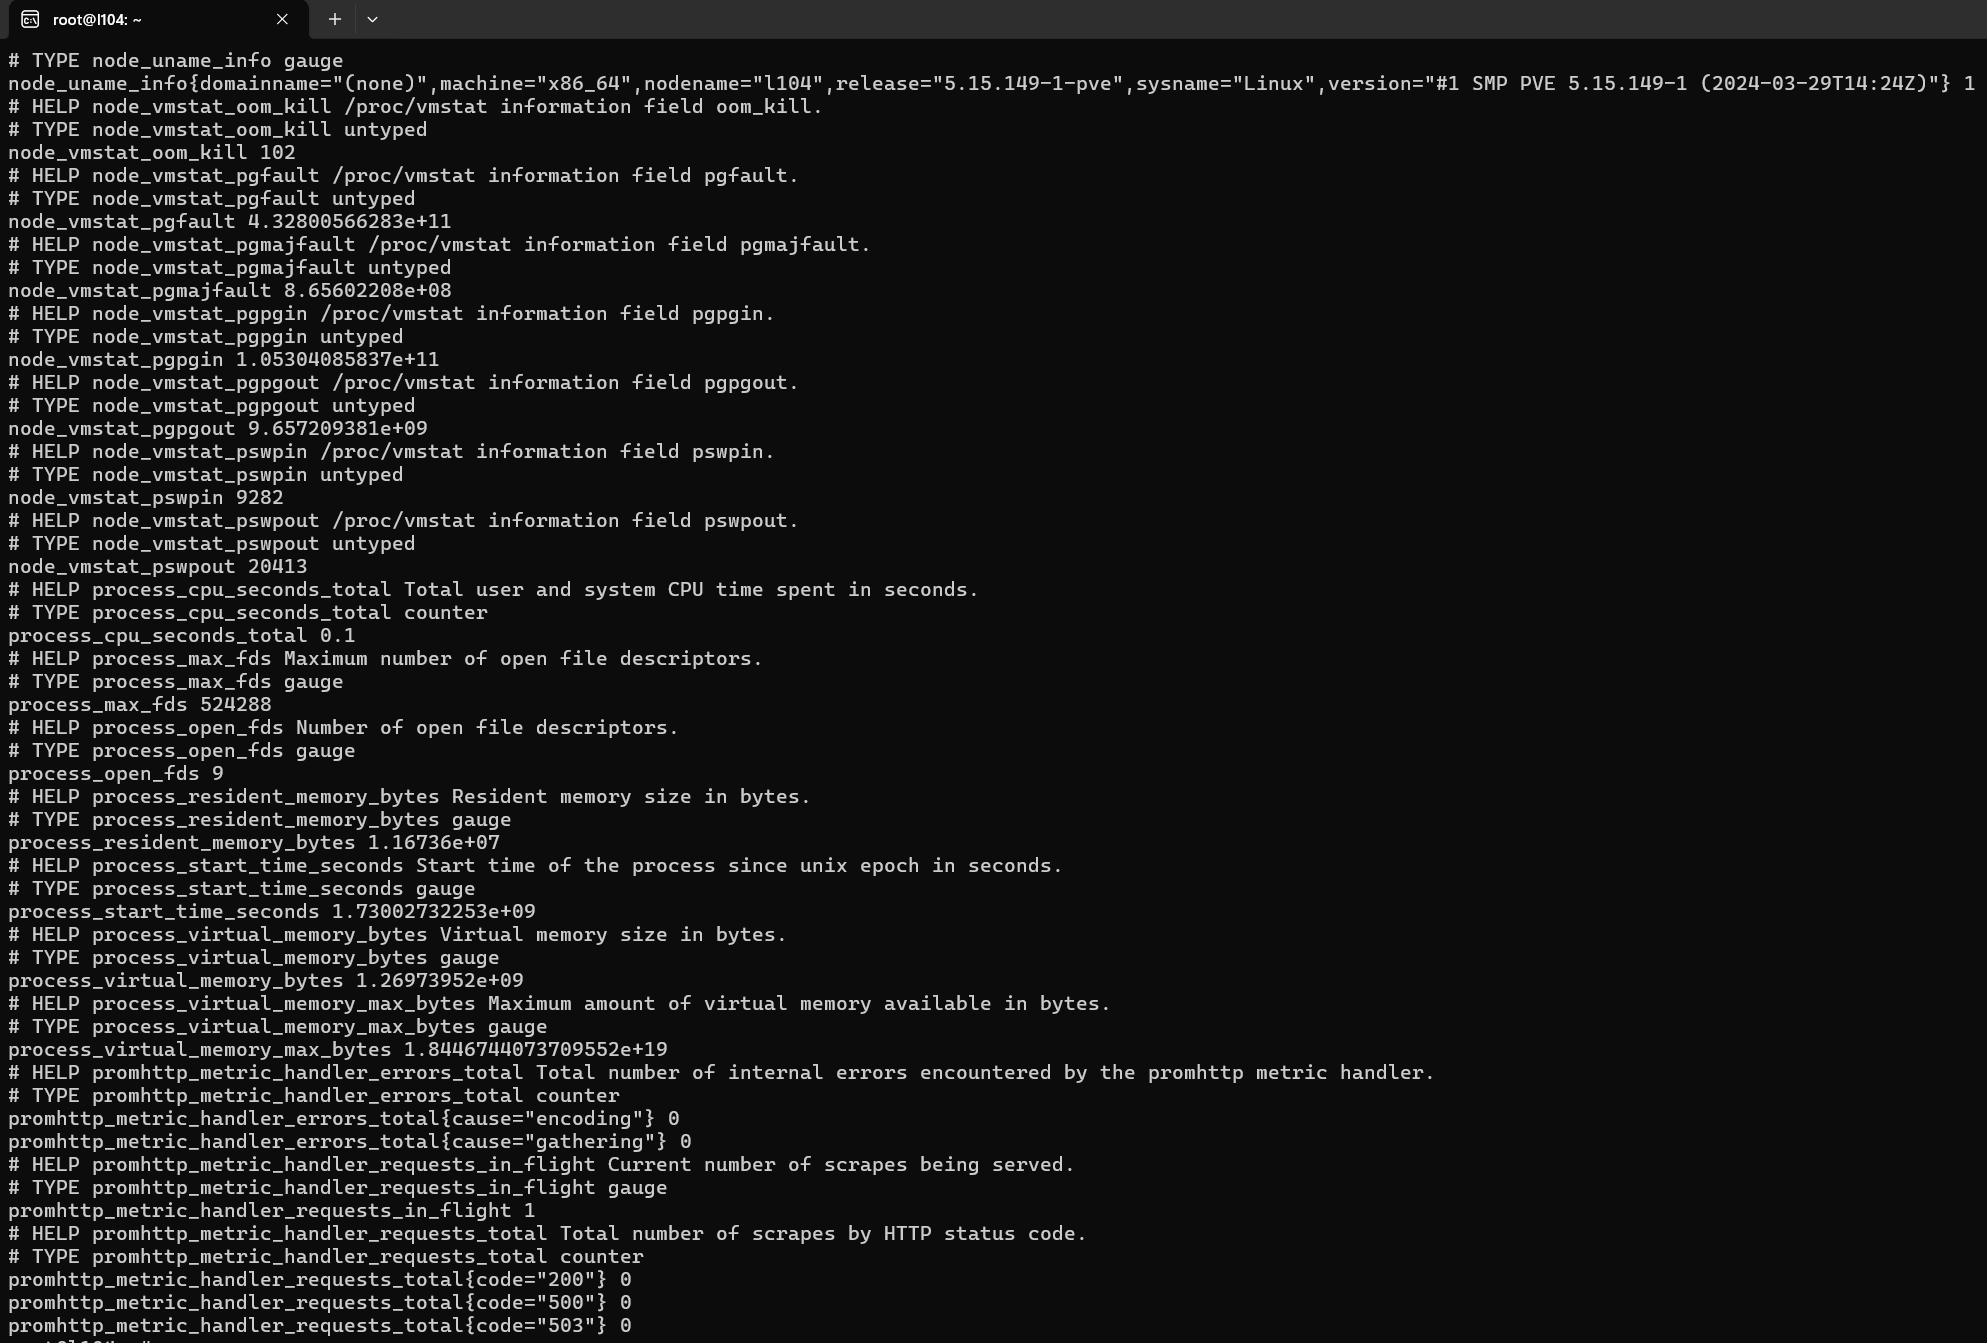
\includegraphics[width=0.75\linewidth]{metrykiNodeExporterRaw.png}
    \caption{Weryfikacja poprawności działania Node Exportera}
    \label{fig:enter-label}
\end{figure}

\subsubsection{Prometheus}

Narzędziem odpowiedzialnym za gromadzenie metryk produkowanych przez Node Exportera jest Prometheus. Konfiguracja tego narzędzia odbywa się przy pomocy pliku \lstinline|.yaml|.

Zaproponowana strategia automatycznej konfiguracji zakłada umieszczenie pliku konfiguracyjnego w repozytorium z infrastrukturą. Repozytorium to zostanie pobrane do specjalnie utworzonego katalogu na serwerze, a przy uruchamianiu Prometheusa plik konfiguracyjny zostanie zamontowany jako \textbf{volume} i przekazany jako odpowiedni argument.

\begin{figure}[H]
    \centering
    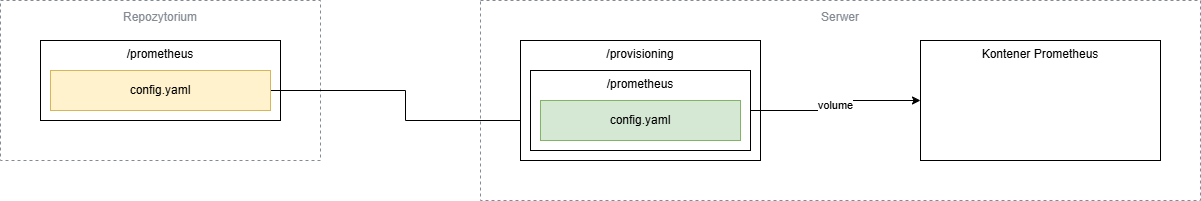
\includegraphics[width=1\linewidth]{diagramProvisionPrometheus.png}
    \caption{Diagram przedstawiający strategię provisioningu Prometheusa}
    \label{fig:enter-label}
\end{figure}

Pierwszym krokiem było przygotowanie pliku konfiguracyjnego, w którym określono adresy dostępnych metryk. Dodatkowo skonfigurowano częstotliwość zbierania danych oraz nazwy poszczególnych metryk.

W przedstawionej konfiguracji Prometheus posiada tylko jedno zadanie (job), którym jest zbieranie metryk z Node Exportera.

\begin{lstlisting}[caption=Plik \texttt{infrastructure/prometheus/prometheus.yml}]
global:
  scrape_interval: 5s
  external_labels:
    monitor: 'node'
scrape_configs:
  - job_name: 'node-exporter'
    static_configs:
      - targets: ['host.docker.internal:9100']

\end{lstlisting}

Następnie przygotowano szablon, który realizuje następujące kroki:
\begin{itemize}
    \item tworzy specjalny katalog na rzeczy związane z Prometheusem,
    \item przechodzi do utworzoneg katalogu,
    \item pobiera repozytorium git,
    \item włącza kontener montując plik konfiguracyjny prometheusa jako volume.
\end{itemize}

\begin{lstlisting}[caption=Plik \texttt{.github/templates/deploy-prometheus/action.yml}]
name: Deploy prometheus

inputs:
  # ssh
  ssh-host:
    required: true
  ssh-username:
    required: true
  ssh-port:
    required: true
  ssh-key:
    required: true

runs:
  using: 'composite'
  steps:
    - name: Deploy prometheus
      uses: appleboy/ssh-action@master
      with:
        host: ${{ inputs.ssh-host }}
        USERNAME: ${{ inputs.ssh-username }}
        PORT: ${{ inputs.ssh-port }}
        KEY: ${{ inputs.ssh-key }}
        script: |
          rm -rf ~/provisioning/prometheus
          mkdir -p ~/provisioning/prometheus
          cd ~/provisioning/prometheus
          git clone https://github.com/ablaszkiewicz/devops-sandbox.git
          cd devops-sandbox/infrastructure/prometheus

          docker run -d \
          --name="monitoring-prometheus" \
          --add-host=host.docker.internal:host-gateway \
          -p 9090:9090 \
          -v $PWD/prometheus.yml:/etc/prometheus/prometheus.yml \
          --restart=always \
          prom/prometheus:v2.49.1
\end{lstlisting}

Na końcu utworzono workflow, który wykorzystuje wspomniany wcześniej szablon.

\begin{lstlisting}[caption=Plik \texttt{.github/workflows/prod-deploy-prometheus.yml}]
name: Deploy prometheus (prod)
on:
  workflow_dispatch: null
  push:
    branches:
      - never
jobs:
  deploy:
    runs-on: ubuntu-latest
    steps:
      - name: Checkout
        uses: actions/checkout@v3
      - name: Stop old containers
        uses: ./.github/templates/stop-old-containers
        with:
          ssh-host: ${{ secrets.SSH_HOST }}
          ssh-username: ${{ secrets.SSH_USER }}
          ssh-port: ${{ secrets.SSH_PORT }}
          ssh-key: ${{ secrets.SSH_KEY }}
          names: 'monitoring-prometheus'
      - name: Deploy prometheus
        uses: ./.github/templates/deploy-prometheus
        with:
          ssh-host: ${{ secrets.SSH_HOST }}
          ssh-username: ${{ secrets.SSH_USER }}
          ssh-port: ${{ secrets.SSH_PORT }}
          ssh-key: ${{ secrets.SSH_KEY }}

\end{lstlisting}

Przetestowano poprawność konfiguracji używając komendy \lstinline|ssh -L 9090:localhost:9090 magisterka|, aby przekierować ruch portu \textbf{Prometheusa} na moją maszynę, po czym odwiedzono \lstinline|http://localhost:9090/targets|, aby zobaczyć skonfigurowane cele.

\begin{figure}[H]
    \centering
    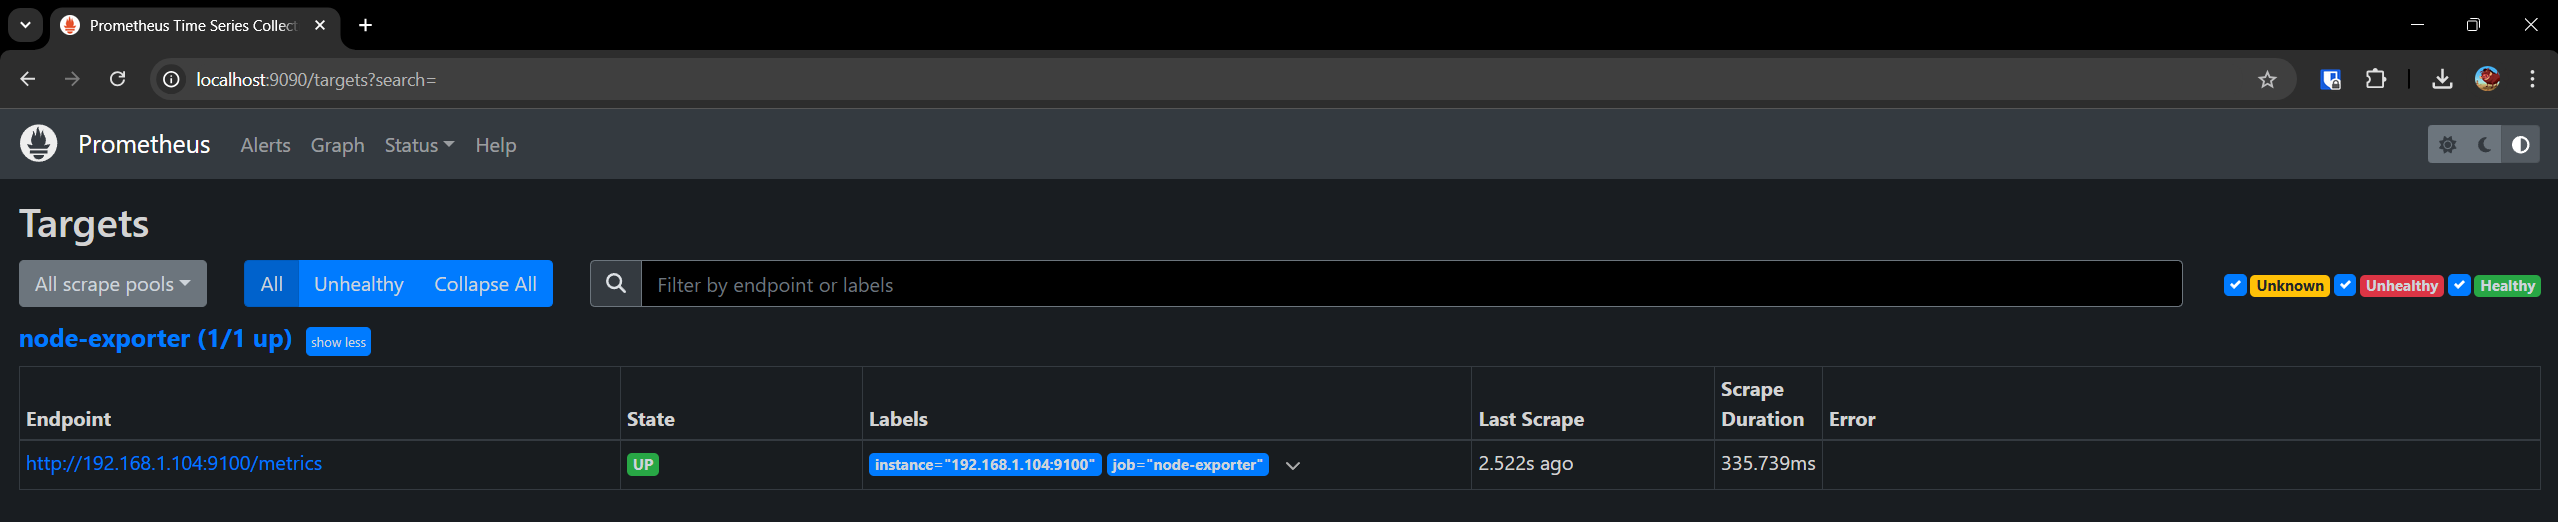
\includegraphics[width=1\linewidth]{prometheusSprawdzenieKonfiguracji.png}
    \caption{Skonfigurowane cele scrapowania w panelu Prometheus}
    \label{fig:enter-label}
\end{figure}

Na powyższym rysunku przedstawiono, że \textbf{Prometheus} poprawnie zbiera dane z \textbf{Node Exportera}.

\subsubsection{Grafana}

Grafana jest narzędziem wizualizacyjnym, które umożliwia przeglądanie i analizowanie danych zbieranych przez Prometheusa. Dzięki integracji z Prometheusem użytkownik może z łatwością tworzyć zaawansowane panele do wizualizacji danych.

Przygotowano szablon, który uruchamia kontener z Grafaną.

\begin{lstlisting}[caption=Plik \texttt{.github/templates/deploy-grafana/action.yml}]
name: Deploy grafana

inputs:
  ssh-host:
    required: true
  ssh-username:
    required: true
  ssh-port:
    required: true
  ssh-key:
    required: true

  grafana-username:
    required: true
  grafana-password:
    required: true

runs:
  using: 'composite'
  steps:
    - name: Deploy grafana
      uses: appleboy/ssh-action@master
      with:
        host: ${{ inputs.ssh-host }}
        USERNAME: ${{ inputs.ssh-username }}
        PORT: ${{ inputs.ssh-port }}
        KEY: ${{ inputs.ssh-key }}
        script: |
          docker run \
            -d \
            -p 2000:3000 \
            --add-host=host.docker.internal:host-gateway \
            --name=monitoring-grafana \
            -e "GF_SECURITY_ADMIN_USER=${{ inputs.grafana-username }}" \
            -e "GF_SECURITY_ADMIN_PASSWORD=${{ inputs.grafana-password }}" \
            --restart=always \
            grafana/grafana:10.3.3
\end{lstlisting}

Dodatkowo utworzono workflow korzystający z powyższego szablonu.

\begin{lstlisting}[caption=Plik \texttt{.github/workflows/prod-deploy-grafana.yml}]
name: Deploy grafana (prod)
on:
  workflow_dispatch: null
  push:
    branches:
      - main
jobs:
  deploy:
    runs-on: ubuntu-latest
    steps:
      - name: Checkout
        uses: actions/checkout@v3
      - name: Stop old containers
        uses: ./.github/templates/stop-old-containers
        with:
          ssh-host: ${{ secrets.SSH_HOST }}
          ssh-username: ${{ secrets.SSH_USER }}
          ssh-port: ${{ secrets.SSH_PORT }}
          ssh-key: ${{ secrets.SSH_KEY }}
          names: 'monitoring-grafana'
      - name: Deploy grafana
        uses: ./.github/templates/deploy-grafana
        with:
          ssh-host: ${{ secrets.SSH_HOST }}
          ssh-username: ${{ secrets.SSH_USER }}
          ssh-port: ${{ secrets.SSH_PORT }}
          ssh-key: ${{ secrets.SSH_KEY }}
          grafana-username: ${{ secrets.MONITORING_USERNAME }}
          grafana-password: ${{ secrets.MONITORING_PASSWORD }}
\end{lstlisting}

Następnie dodano sekrety uwierzytelnienia w repozytorium.

\begin{figure}[H]
    \centering
    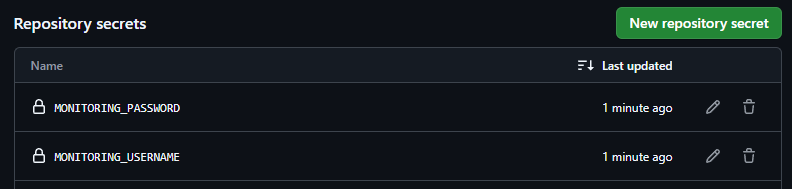
\includegraphics[width=1\linewidth]{sekretyGrafana.png}
    \caption{Sekrety uwierzytelniania do grafany dodane do repozytorium}
    \label{fig:enter-label}
\end{figure}

Skonfigurowano również domenę w usłudze Cloudflare.

\begin{figure}[H]
    \centering
    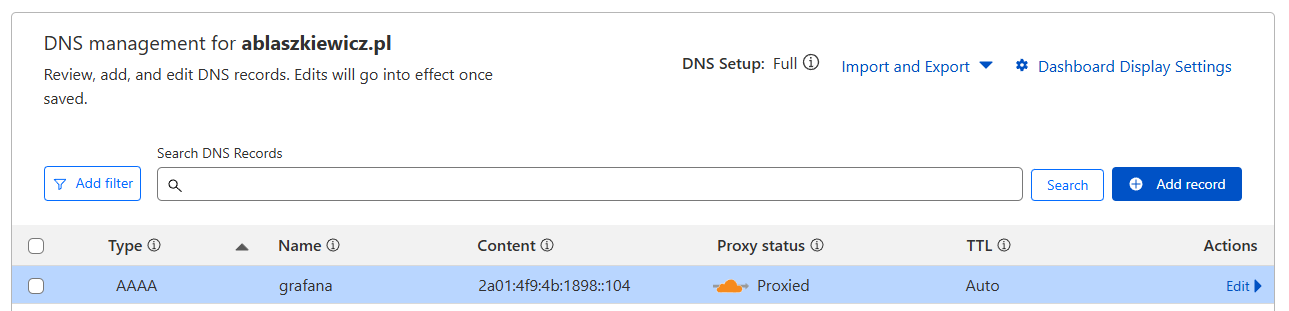
\includegraphics[width=1\linewidth]{grafanaDNS.png}
    \caption{Ustawienia DNS Grafana}
    \label{fig:enter-label}
\end{figure}

Ostatnim krokiem była modyfikacja konfiguracji reverse proxy, aby przekierowywać ruch z \lstinline|grafana.ablaszkiewicz.pl| na \lstinline|localhost:2000|, gdzie wdrożona jest Grafana.

\begin{lstlisting}[caption=Zaktualizowany plik \texttt{infrastructure/reverse-proxy-shared/config}]
grafana.ablaszkiewicz.pl=http://192.168.1.104:2000
dev.ablaszkiewicz.pl=http://192.168.1.104:4080
ablaszkiewicz.pl=http://192.168.1.104:3080
\end{lstlisting}

Po ukończeniu konfiguracji można uzyskać dostęp do Grafany.

\begin{figure}[H]
    \centering
    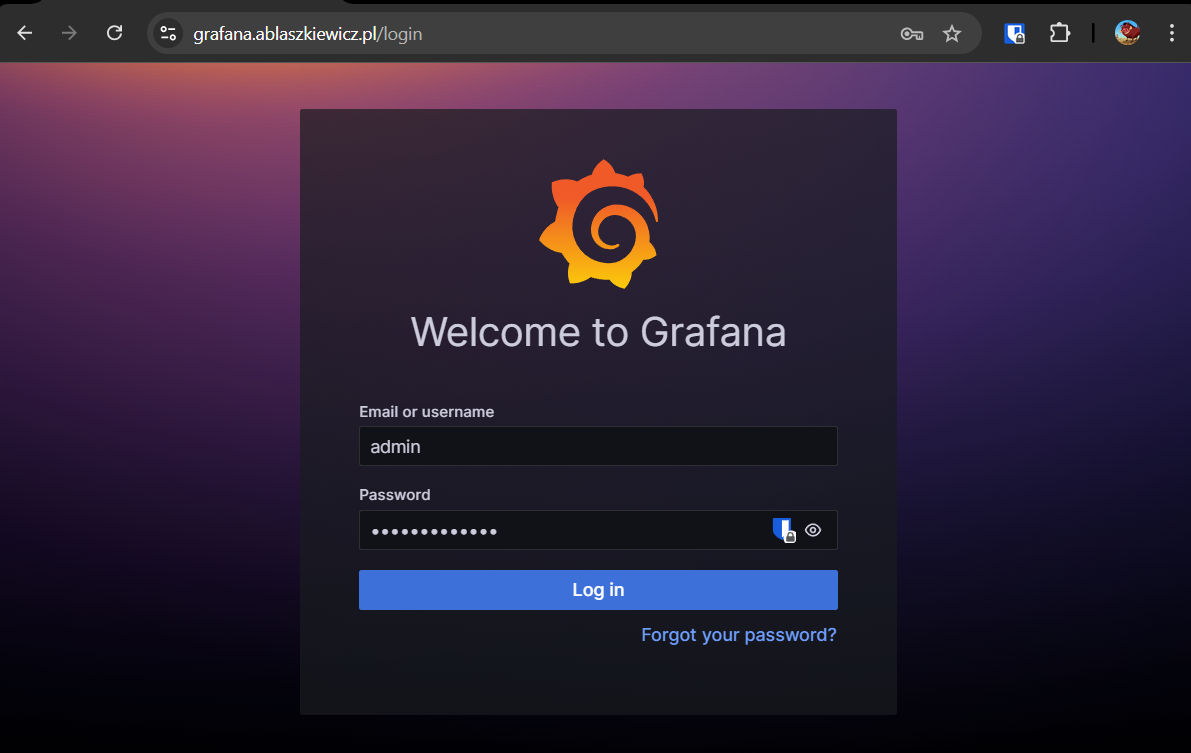
\includegraphics[width=0.75\linewidth]{grafanaLogowanie.png}
    \caption{Odwiedzenie adresu Grafany}
    \label{fig:enter-label}
\end{figure}

Uwierzytelnienie przebiega pomyślnie przy użyciu danych zapisanych w sekretach.

\begin{figure}[H]
    \centering
    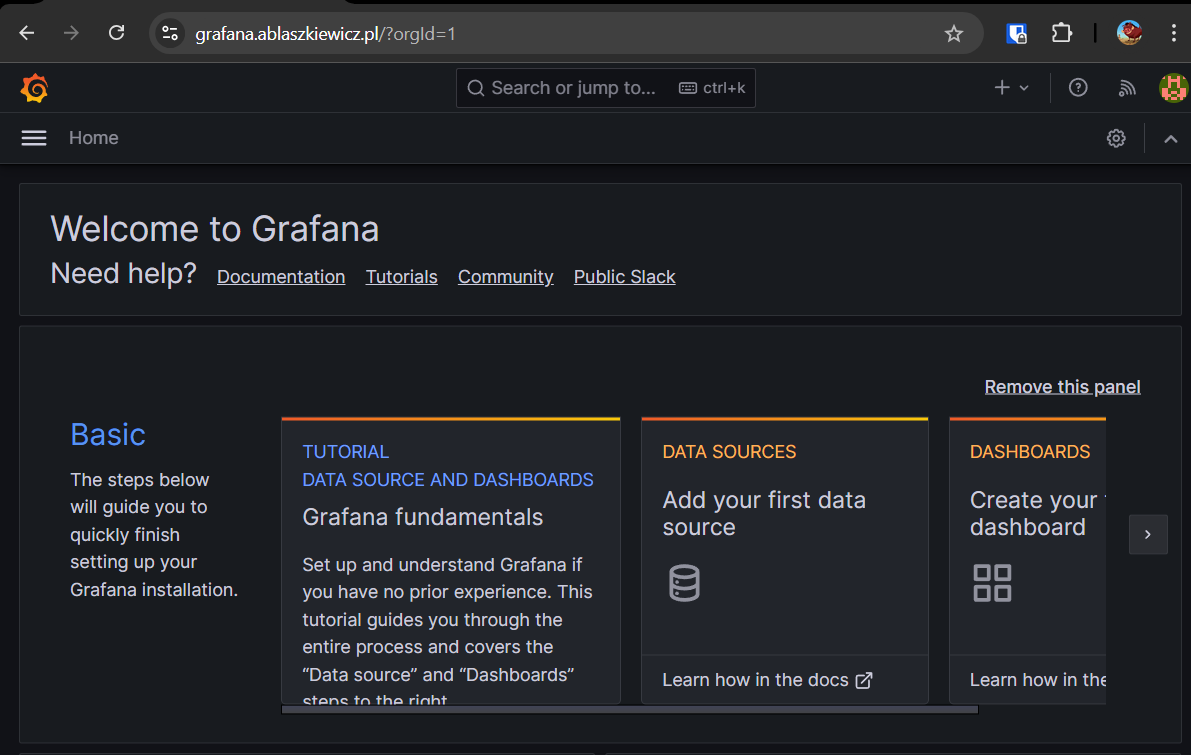
\includegraphics[width=0.75\linewidth]{grafanaPomyslneZalogowanie.png}
    \caption{Pomyślne zalogowanie do Grafany}
    \label{fig:enter-label}
\end{figure}

Aby sprawdzić poprawność konfiguracji, dodano Prometheusa jako źródło danych (\textit{Data Source}) w zakładce Data Sources, podając odpowiedni adres.

\begin{figure}[H]
    \centering
    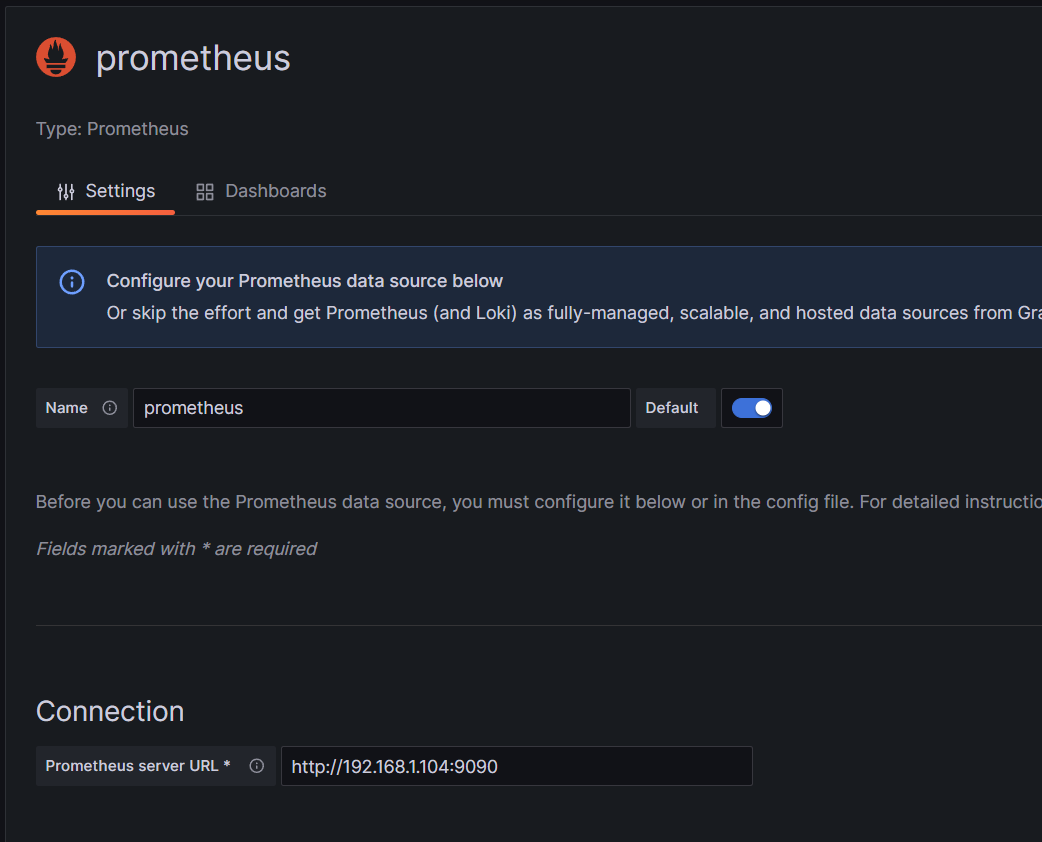
\includegraphics[width=1\linewidth]{prometheusDodanieGrafana.png}
    \caption{Dodanie Prometheusa w Grafanie}
    \label{fig:enter-label}
\end{figure}

Po zapisaniu konfiguracji pojawiła się informacja potwierdzająca poprawne połączenie.

\begin{figure}[H]
    \centering
    
\includegraphics[width=1\linewidth]{grafanaPoprawnyPrometheus.png}
    \caption{Wiadomość sygnalizująca poprawne skonfigurowanie Prometheusa}
    \label{fig:enter-label}
\end{figure}

Aby uzyskać wizualizację statystyk serwera, utworzono nowy dashboard w Grafanie, oparty na dashboardzie udostępnionym przez społeczność pod adresem \lstinline|https://grafana.com/grafana/dashboards/1860-node-exporter-full/|.

Po zapisaniu ustawień możliwe jest wyświetlenie zwizualizowanych statystyk serwera.

Aby uniknąć utraty konfiguracji w przypadku restartu kontenera, przeniesiono konfigurację Grafany do plików montowanych przy uruchamianiu kontenera, podobnie jak w przypadku Prometheusa.

\begin{figure}[H]
    \centering
    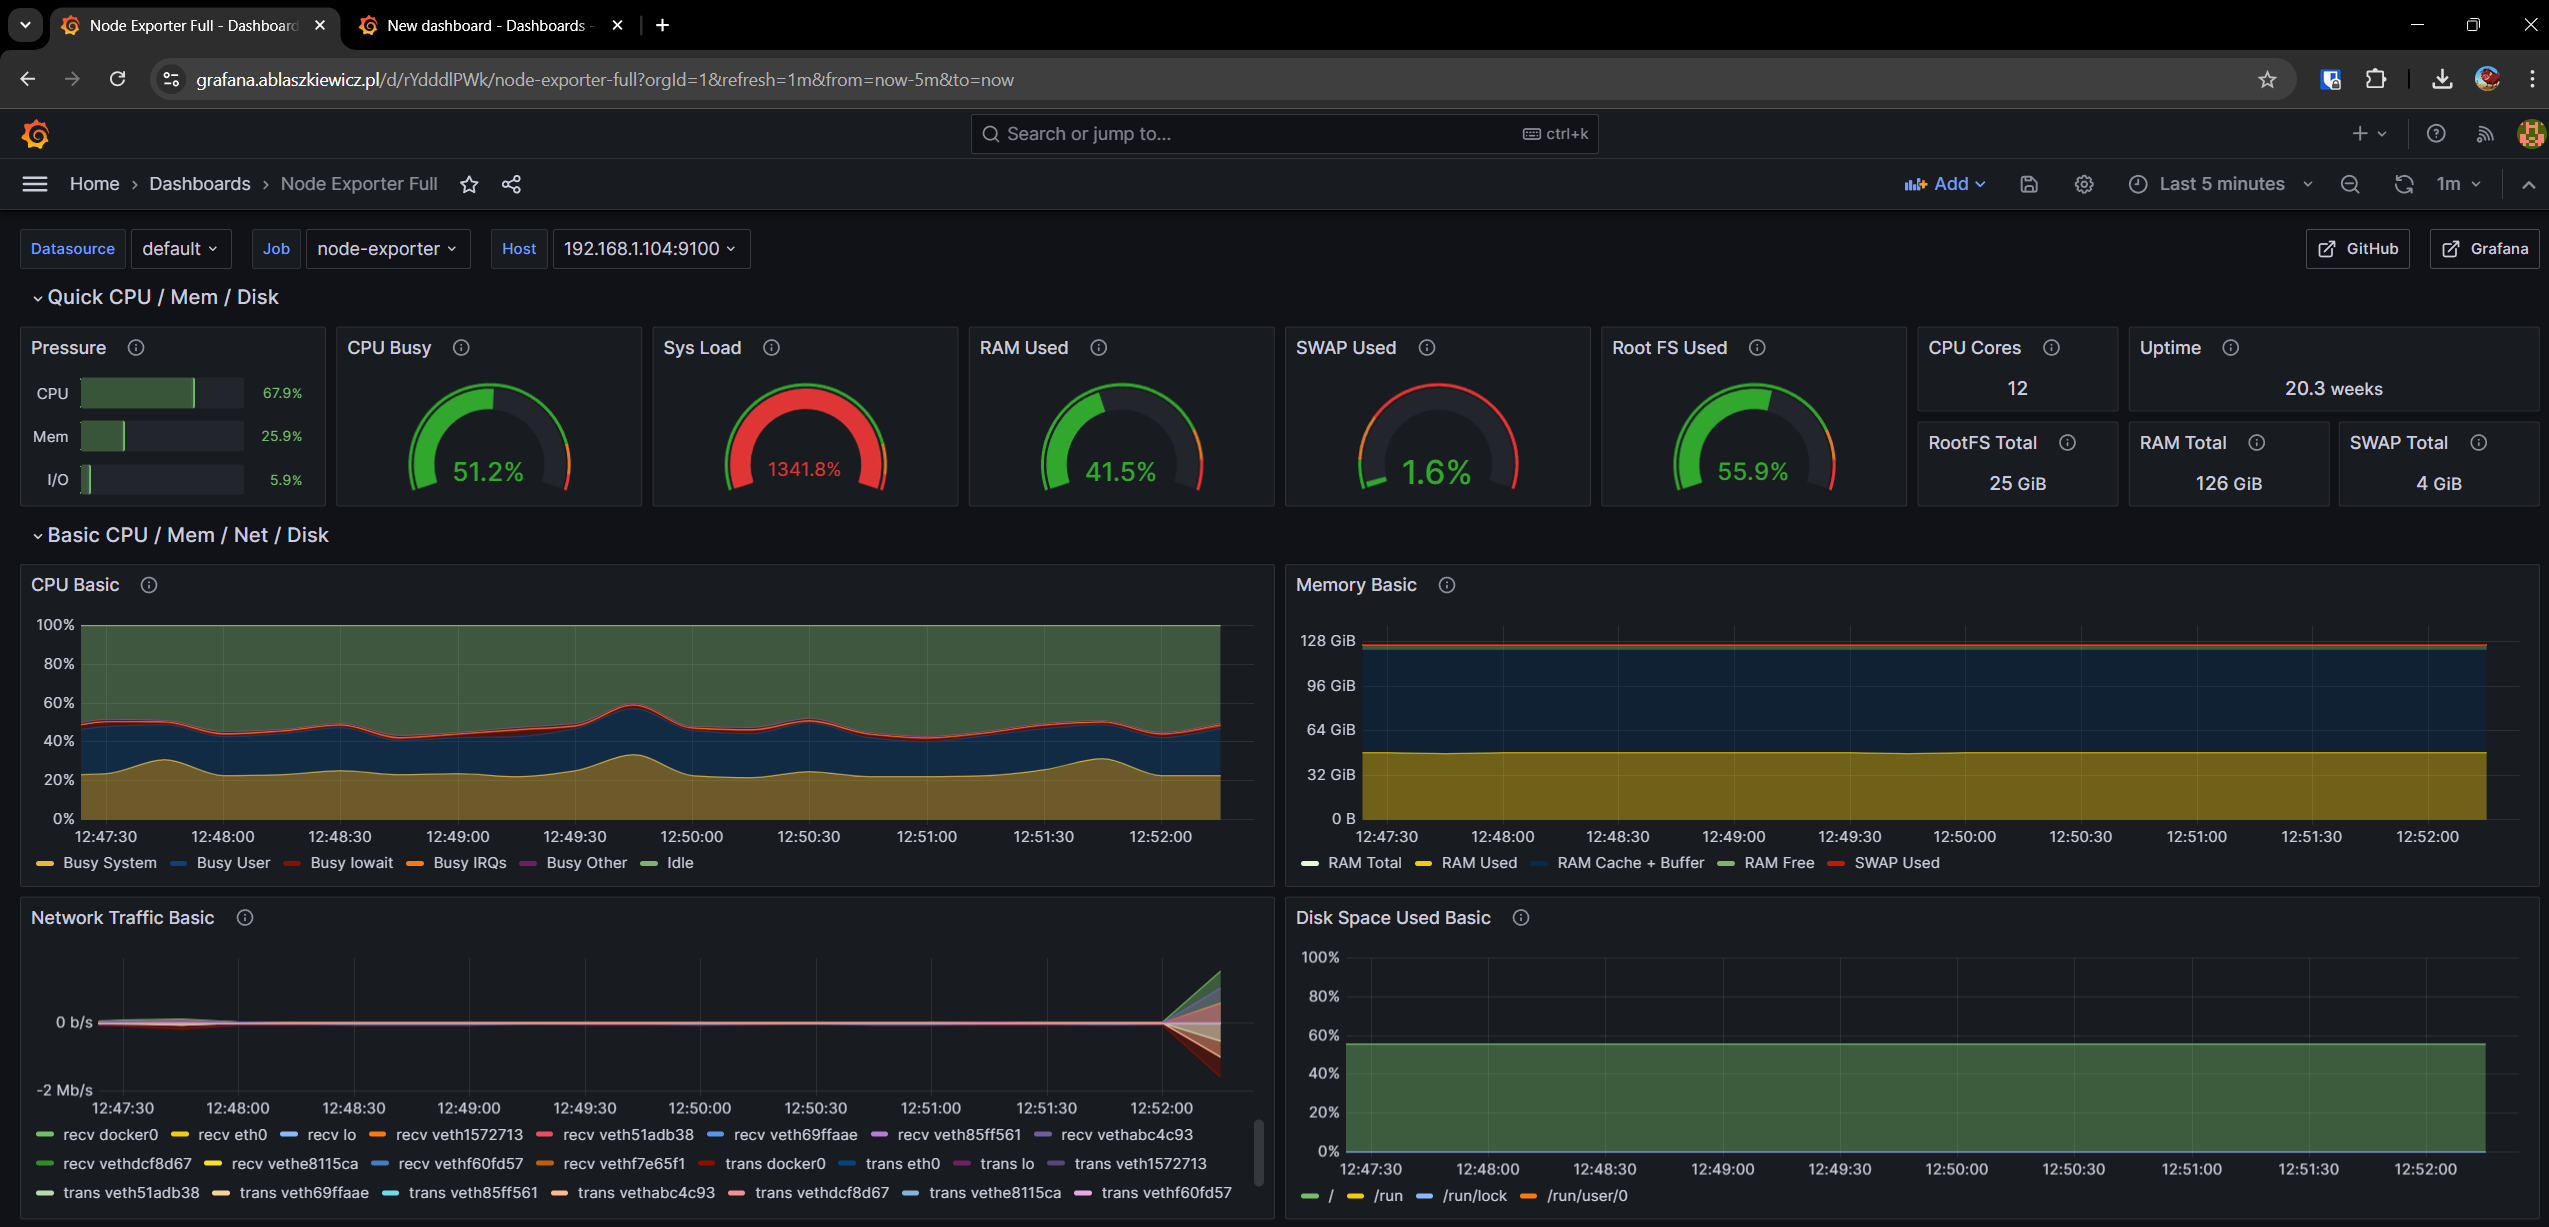
\includegraphics[width=1\linewidth]{grafanaNodeExporterDashboard.png}
    \caption{Dashboard Node Exportera w Grafanie}
    \label{fig:enter-label}
\end{figure}

\begin{lstlisting}[caption=Plik \texttt{infrastructure/grafana/datasources/datasources.yml}]
apiVersion: 1

datasources:
  - name: Prometheus
    type: prometheus
    access: proxy
    uid: prometheus_datasource_uid
    url: http://192.168.1.104:9090
\end{lstlisting}

\begin{lstlisting}[caption=Plik \texttt{infrastructure/grafana/dashboards/dashboards.yml}]
apiVersion: 1

providers:
  - name: dashboards
    type: file
    updateIntervalSeconds: 30
    options:
      path: /etc/grafana/provisioning/dashboards
      foldersFromFilesStructure: true
\end{lstlisting}

Korzystając z interfejsu Grafany, wyeksportowano aktualny dashboard w formacie JSON i zapisano go w pliku \lstinline|infrastructure/grafana/dashboards/node-exporter.json|.

Ostatecznie zmodyfikowano szablon wdrożeniowy Grafany, aby montował nowo utworzone pliki konfiguracyjne jako \textbf{volume}.

\begin{lstlisting}[caption=Zmodyfikowany plik \texttt{.github/templates/deploy-grafana/action.yml}]
name: Deploy grafana

inputs:
  ssh-host:
    required: true
  ssh-username:
    required: true
  ssh-port:
    required: true
  ssh-key:
    required: true

  grafana-username:
    required: true
  grafana-password:
    required: true

runs:
  using: 'composite'
  steps:
    - name: Deploy grafana
      uses: appleboy/ssh-action@master
      with:
        host: ${{ inputs.ssh-host }}
        USERNAME: ${{ inputs.ssh-username }}
        PORT: ${{ inputs.ssh-port }}
        KEY: ${{ inputs.ssh-key }}
        script: |
          rm -rf ~/provisioning/grafana
          mkdir -p ~/provisioning/grafana
          cd ~/provisioning/grafana
          git clone https://github.com/ablaszkiewicz/devops-sandbox.git
          cd devops-sandbox/infrastructure/grafana


          docker run \
            -d \
            -p 2000:3000 \
            --add-host=host.docker.internal:host-gateway \
            --name=monitoring-grafana \
            -e "GF_INSTALL_PLUGINS=grafana-worldmap-panel" \
            -e "GF_PATHS_PROVISIONING=/etc/grafana/provisioning" \
            -e "GF_SECURITY_ADMIN_USER=${{ inputs.grafana-username }}" \
            -e "GF_SECURITY_ADMIN_PASSWORD=${{ inputs.grafana-password }}" \
            -v $PWD/dashboards:/etc/grafana/provisioning/dashboards \
            -v $PWD/datasources:/etc/grafana/provisioning/datasources \
            --restart=always \
            grafana/grafana:10.3.3
\end{lstlisting}

Po ponownym wdrożeniu kontenera Grafany konfiguracja źródeł danych i dashboardów została zachowana.

\subsubsection{Alerty grafana}

\begin{figure}[H]
    \centering
    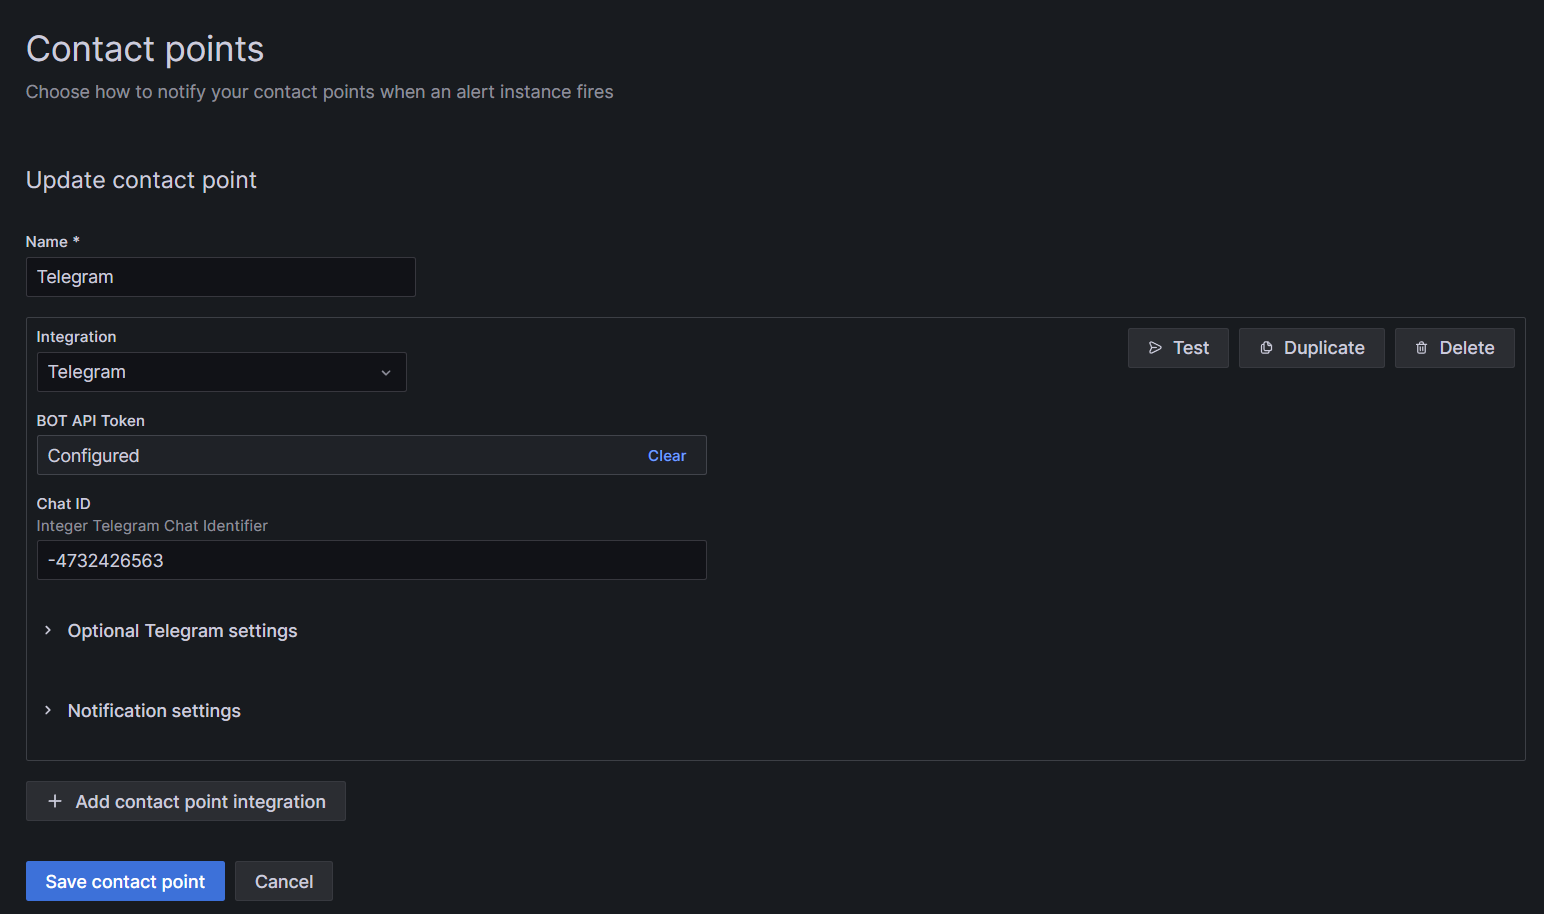
\includegraphics[width=1\linewidth]{konfiguracjaContactPointGrafana.png}
    \caption{Konfiguracja contact point w Grafanie}
    \label{fig:enter-label}
\end{figure}

\begin{figure}[H]
    \centering
    \includegraphics[width=1\linewidth]{konfiguracjaAlertGrafana.png}
    \caption{Konfiguracja alertu w Grafanie}
    \label{fig:enter-label}
\end{figure}

\begin{figure}[H]
    \centering
    \includegraphics[width=1\linewidth]{alertGrafana.png}
    \caption{Alert widoczny na telegramie, który przyszedł z Grafany}
    \label{fig:enter-label}
\end{figure}

\subsubsection{Alerty Grafana}

Aby w sposób zautomatyzowany powiadamiać administratora o potencjalnych nieprawidłowościach w działaniu systemu, w narzędziu Grafana skonfigurowano mechanizm alertów. Proces ten obejmuje przede wszystkim zdefiniowanie \textit{contact point}, czyli kanału dystrybucji powiadomień (np.\ komunikator Telegram, e-mail lub inna wybrana usługa), a następnie utworzenie reguły (tzw.\ \textit{alert rule}), która określa warunki wyzwalające wysłanie alertu.

Pierwszym etapem konfiguracji systemu alertów w Grafanie jest dodanie tzw.\ \textit{contact point}, czyli miejsca docelowego, do którego kierowane będą powiadomienia o pojawiających się zdarzeniach krytycznych (rys.\ref{fig:contact-point-grafana}). W tym celu należy określić typ kanału (womawianym środowisku użyto komunikatora Telegram) oraz wprowadzić niezbędne dane uwierzytelniające i konfiguracje połączenia.

\begin{figure}[H] \centering \includegraphics[width=0.9\linewidth]{konfiguracjaContactPointGrafana.png} \caption{Konfiguracja \textit{contact point} w Grafanie} \label{fig:contact-point-grafana} \end{figure}

Kolejnym krokiem jest utworzenie reguły alertu, która określa warunki wysyłania powiadomień (rys.~\ref{fig:alert-rule-grafana}). Reguła ta może opierać się na dowolnych danych dostępnych w Grafanie, np.\ metrykach z Prometheusa. Administrator definiuje metrykę lub zapytanie (ang.\ \textit{query}), a następnie ustawia progi (np.\ zużycie pamięci, obciążenie CPU) lub warunki braku odpowiedzi serwisu, powodujące powstanie stanu \textit{alerting} i wygenerowanie powiadomienia.

\begin{figure}[H] \centering \includegraphics[width=0.9\linewidth]{konfiguracjaAlertGrafana.png} \caption{Konfiguracja reguły alertu w Grafanie} \label{fig:alert-rule-grafana} \end{figure}

Po spełnieniu zadeklarowanych w regule warunków (np.\ przekroczeniu ustalonego progu metryki) alert przechodzi w stan \textit{firing}, a Grafana wysyła powiadomienie do skonfigurowanego \textit{contact point}. Dzięki takiemu podejściu administrator ma możliwość szybkiej reakcji na potencjalne problemy. Na rysunku~\ref{fig:alert-grafana-telegram} zaprezentowano przykład alertu odebranego w komunikatorze Telegram.

\begin{figure}[H] \centering \includegraphics[width=0.9\linewidth]{alertGrafana.png} \caption{Przykładowy alert z Grafany wysłany do Telegrama} \label{fig:alert-grafana-telegram} \end{figure}

Dzięki konfiguracji alertów w Grafanie zespół administratorów otrzymuje szybkie i~zautomatyzowane powiadomienia o występujących problemach (np.\ przeciążeniu serwera, nieosiągalności usługi czy przekroczeniu istotnych progów metryk). Pozwala to na błyskawiczne podjęcie działań naprawczych oraz minimalizuje ryzyko dłuższych przestojów czy awarii.

\subsection{Porównanie Grafany i Uptime Kuma}


Uptime Kuma oraz Grafana to narzędzia służące do monitorowania środowisk IT, jednak różnią się one zarówno zakresem funkcjonalności, jak i stopniem zaawansowania konfiguracji. Poniżej przedstawiono kluczowe cechy obu rozwiązań, uzupełnione o tabelaryczne zestawienie.

\paragraph{Zakres i funkcjonalność}
\begin{itemize}
    \item \textbf{Uptime Kuma} -- skupia się przede wszystkim na monitorowaniu dostępności usług poprzez wysyłanie żądań HTTP (pingi do endpointów) w ustalonych interwałach. Narzędzie to w sposób intuicyjny pozwala na obserwację podstawowych wskaźników \emph{uptime} i \emph{downtime},
    \item \textbf{Grafana} -- pełni rolę kompleksowego rozwiązania do wizualizacji i analizy danych. Dzięki integracji z wieloma źródłami metryk (np.\ Prometheus, InfluxDB, ElasticSearch), użytkownicy mogą tworzyć rozbudowane dashboardy i w czasie rzeczywistym analizować obciążenie serwera, wykorzystanie zasobów czy inne niestandardowe metryki.
\end{itemize}

\paragraph{Łatwość instalacji i konfiguracji}
\begin{itemize}
    \item \textbf{Uptime Kuma} -- charakteryzuje się prostotą instalacji i szybką konfiguracją. Narzędzie może zostać uruchomione w kontenerze Docker (bez rozbudowanych zależności) i po krótkim wstępnym skonfigurowaniu od razu dostarcza podstawowy panel monitorujący,
    \item \textbf{Grafana} -- sama instalacja Grafany (również w kontenerze Docker) nie jest skomplikowana, jednak aby w pełni wykorzystać jej możliwości, należy dodatkowo zintegrować ją z dostawcami danych (np.\ Prometheus). Proces ten wymaga bardziej zaawansowanej konfiguracji i zrozumienia modelu danych.
\end{itemize}

\paragraph{Monitorowanie i alertowanie}
\begin{itemize}
    \item \textbf{Uptime Kuma} -- zapewnia podstawowe alerty (np.\ Telegram, e-mail) w przypadku wykrycia niedostępności usługi. Jest to intuicyjne w konfiguracji i wystarczające do prostych zastosowań, takich jak sprawdzanie, czy dana usługa HTTP odpowiada,
    \item \textbf{Grafana} -- posiada bardziej rozbudowany system alertów (m.in.\ stany \emph{warning}, \emph{critical}) oparty o reguły zdefiniowane na podstawie metryk zintegrowanych źródeł. Umożliwia tworzenie złożonych warunków alertowania oraz powiadomień przez różne kanały (Slack, e-mail, Telegram, itp.). 
\end{itemize}

\paragraph{Rozszerzalność i elastyczność}
\begin{itemize}
    \item \textbf{Uptime Kuma} -- koncentruje się na jednym głównym zadaniu (monitorowanie dostępności). Nie oferuje rozbudowanych możliwości wizualizacji czy analizy, choć można go zintegrować z innymi narzędziami w środowisku,
    \item \textbf{Grafana} -- jest wysoce konfigurowalna i rozszerzalna poprzez \emph{pluginy}, gotowe panele społeczności (tzw.\ \emph{community dashboards}) oraz integracje z wieloma usługami. Pozwala to na pełen wgląd w stan i wydajność aplikacji.
\end{itemize}

\paragraph{Przykładowe zastosowania}
\begin{itemize}
    \item \textbf{Uptime Kuma} -- szybkie uruchomienie i monitorowanie kluczowych endpointów aplikacji internetowych, prosty mechanizm alertowania o niedostępności,
    \item \textbf{Grafana} -- zaawansowana analityka, przeglądanie metryk historycznych, agregacja danych z wielu źródeł (logi, metryki, zdarzenia), możliwość tworzenia złożonych raportów.
\end{itemize}

\begin{table}[H]
\centering
\begin{tabular}{|p{4.5cm}|p{4.5cm}|p{4.5cm}|}
\hline
\textbf{Cecha}                  & \textbf{Uptime Kuma}                                                                 & \textbf{Grafana}                                                         \\ \hline
\textbf{Główne zadanie}         & Monitorowanie dostępności i czasu reakcji usług                                     & Kompleksowa wizualizacja i analiza danych z różnych źródeł               \\ \hline
\textbf{Łatwość instalacji}     & Bardzo prosta (kontener Docker, minimalna konfiguracja)                             & Również prosta, ale pełny potencjał wymaga integracji z zewnętrznymi DB   \\ \hline
\textbf{Alerty}                 & Proste powiadomienia (Telegram, e-mail, \emph{push})                                & Zaawansowane (reguły warunkowe, wielopoziomowe stany, różne kanały)       \\ \hline
\textbf{Dashboardy}             & Podstawowy panel z listą monitorowanych usług                                       & Rozbudowane, konfigurowalne panele i wizualizacje                         \\ \hline
\textbf{Skalowalność}           & Możliwe skalowanie w poziomie (więcej monitorów, wiele instancji Docker)           & Łatwe skalowanie i integracja z wieloma źródłami (Prometheus, InfluxDB)   \\ \hline
\textbf{Próg wejścia}           & Niski (łatwość konfiguracji, szybkie uruchomienie)                                   & Wysoki (konieczna znajomość źródeł danych i reguł alertowania) \\ \hline
\textbf{Zaawansowana analityka} & Ograniczona głównie do wykrywania stanu \emph{up/down}                               & Bogate możliwości (statystyki, korelacje, współdziałanie z innymi narzędziami) \\ \hline
\end{tabular}
\caption{Porównanie Uptime Kuma i Grafana}
\label{tab:porownanie-uptime-kuma-grafana}
\end{table}

Podsumowując, \textbf{Uptime Kuma} jest doskonałym wyborem, gdy celem jest szybkie wdrożenie podstawowego monitoringu dostępności usług oraz prostych alertów. Z kolei \textbf{Grafana} wyróżnia się znacznie szerszym zakresem zastosowań, zwłaszcza w obszarach zaawansowanej analizy i wizualizacji danych. W zależności od potrzeb projektu, oba rozwiązania można również zintegrować, aby uzyskać z jednej strony \emph{uptime monitoring}, a z drugiej -- pełną analitykę i wgląd w szczegółowe metryki. 


\begin{thebibliography}{9}

\bibitem{flickr}
John Allspaw, Paul Hammond, "10+ Deploys per Day: Dev and Ops Cooperation at Flickr", 2009. [Prezentacja] \url{https://www.slideshare.net/jallspaw/10-deploys-per-day-dev-and-ops-cooperation-at-flickr} [Dostęp: 20 listopada 2024]

\bibitem{devOpsDays}
"DevOpsDays". [Strona internetowa] \url{https://devopsdays.org/} [Dostęp: 20 listopada 2024]

\bibitem{devOpsHandbook}
Gene Kim, Patrick Debois, Professor John Willis, Jez Humble, "The DevOPS Handbook: How to Create World-Class Agility, Reliability, and Security in Technology Organizations", 2016.

\bibitem{damonEdwards}
Damon Edwards, "What is DevOps?", 2010. [Blog] \url{http://dev2ops.org/2010/02/what-is-devops/} [Dostęp: 20 listopada 2024]

\bibitem{cdDockerJenkins}
Rafał Leszko, "Building CI/CD using Docker and Jenkins", 2017.

\bibitem{royceWaterfall}
Winston Royce, "Managing the Development of Large Software Systems", 1970.

\bibitem{stateOfDevops}
"2023 State of DevOps", 2023. [Blog] \url{https://www.splunk.com/en_us/blog/learn/state-of-devops.html} [Dostęp: 21 listopada 2024]

\bibitem{babisha}
Bhabishya Gorung, "A comparative analysis of create-react-app (CRA) and Vite for React.js projects", 2024. [Praca] \url{https://www.theseus.fi/bitstream/handle/10024/860241/Gurung_Bhabishya.pdf?sequence=2&isAllowed=y} [Dostęp: 21 listopada 2024]

\bibitem{cleanArchitecture}
Robert C. Martin, "Clean Architecture: A Craftsman's Guide to Software Structure and Design", 2017.

\bibitem{understandingIdempotency}
Thalia Barrera, "Understanding Idempotency: A Key to Reliable and Scalable Data Pipelines", 2023. [Blog] \url{https://airbyte.com/data-engineering-resources/idempotency-in-data-pipelines} [Dostęp: 21 listopada 2024]

\bibitem{continuousDelivery}
Jez Humble, David Farley, "Continuous Delivery: Reliable Software Releases through Build, Test, and Deployment Automation", 2010.

\bibitem{characterizationFramework}
Fugetta Alfonso, Hall Richard S., Carzaniga Antonio, Heimbigner Dennis M, "A Characterization Framework for Software Deployment Technologies", 2010. [Praca] \url{https://scholar.colorado.edu/concern/reports/v405sb15g} [Dostęp: 22 listopada 2024]

\bibitem{efficientDocker}
Mokshith Reddy Eda, N. Srinivasu, Suneetha Bulla, "Mokshith Reddy Eda, N. Srinivasu, Suneetha Bulla", 2023. [Praca] \url{https://www.researchgate.net/publication/373346783_Efficient_Docker_Image_Optimization_using_Multi-Stage_Builds_and_Nginx_for_Enhanced_Application_Deployment} [Dostęp: 22 listopada 2024]

\bibitem{smallerContainers}
Tonis Tiigi, "How to Build Smaller Container Images: Docker Multi-Stage Builds", 2024. [Praca] \url{https://labs.iximiuz.com/tutorials/docker-multi-stage-builds} [Dostęp: 22 listopada 2024]

\bibitem{reduceDockerImages}
Travis Media, "How to Significantly Reduce Your Docker Images with Multi-Stage Builds", 2010. [Blog] \url{https://travis.media/blog/docker-multi-stage-builds/} [Dostęp: 23 listopada 2024]

\bibitem{AzureDevOpsGitHubActionsComparison}
Melanie, "Azure DevOps vs GitHub Actions: Which is the best CI/CD tool?", 2023. [Artykuł] \url{https://datascientest.com/en/azure-devops-vs-github-actions-which-is-the-best-ci-cd-tool} [Dostęp: 23 listopada 2024]

\bibitem{GitLabAzureDevOpsComparison}
Piotr Zięba, "Porównanie narzędzi DevOps: GitLab i Azure DevOps", 2020. [Blog] \url{https://deviniti.com/pl/blog/devops-pl/porownanie-narzedzi-devops-gitlab-azure/} [Dostęp: 23 listopada 2024]

\bibitem{CircleCIGitHubActionsGitLab}
Vince Power, "CircleCI vs. GitHub Actions vs. GitLab: Key Differences", 2023. [Blog] \url{https://saucelabs.com/resources/blog/circleci-vs-github-actions-vs-gitlab-key-differences} [Dostęp: 24 listopada 2024]

\bibitem{GitHubActionsImporter}
GitHub, "GitHub Actions Importer". [Repozytorium] \url{https://github.com/actions/importer-labs} [Dostęp: 24 listopada 2024]

\bibitem{BabelWikipedia}
Wikipedia, "Babel (transcompiler)". [Artykuł] \url{https://en.wikipedia.org/wiki/Babel_%28transcompiler%29} [Dostęp: 24 listopada 2024]

\bibitem{BabelDailyDev}
DailyDev, "Typescript Transpiler Tools Comparison". [Artykuł] \url{https://daily.dev/blog/typescript-transpiler-tools-comparison?utm_source=chatgpt.com} [Dostęp: 25 listopada 2024]

\bibitem{BabelLogRocket}
LogRocket, "Why you should use SWC (and not Babel)". [Artykuł] \url{https://blog.logrocket.com/why-you-should-use-swc} [Dostęp: 25 listopada 2024]

\bibitem{DevCra}
DevTo, "Goodbye create-react-app". [Artykuł] \url{https://dev.to/ag2byte/create-react-app-is-officially-dead-h7o} [Dostęp: 25 listopada 2024]

\bibitem{ViteSite}
Vite. [Strona] \url{https://vite.dev/} [Dostęp: 26 listopada 2024]

\bibitem{NodemonArticle}
Refine, "How to Use Nodemon to Automatically Restart Node.js Applications". [Artykuł] \url{https://refine.dev/blog/nodemon/} [Dostęp: 26 listopada 2024]

\bibitem{NodejsAviary}
Aviary, "Node.js – przewodnik po środowisku uruchomieniowym JavaScript". [Artykuł] \url{https://aviary.pl/node-js/} [Dostęp: 26 listopada 2024]

\bibitem{DockerAlpine}
Docker, "How to Use the Alpine Docker Official Image". [Artykuł] \url{https://www.docker.com/blog/how-to-use-the-alpine-docker-official-image/} [Dostęp: 27 listopada 2024]

\bibitem{MediumDistroless}
Pratik Nalawade, "Distroless Images in Docker: Streamlining Containers for Security and Efficiency". [Artykuł] \url{https://medium.com/@nalawade1000work/distroless-images-in-docker-streamlining-containers-for-security-and-efficiency-42372d1b7fb9} [Dostęp: 27 listopada 2024]

\bibitem{Krakweb}
Krakweb, "4 najpopularniejsze mechanizmy uwierzytelniania". [Artykuł] \url{https://www.krakweb.pl/4-najpopularniejsze-mechanizmy-uwierzytelniania-klucze-ssh-tokeny-oauth-certyfikaty-ssl-oraz-dane-uwierzytelniajace-loginy-i-hasla} [Dostęp: 27 listopada 2024]

\bibitem{NginxDocs}
Nginx, "NGINX Reverse Proxy". [Dokumentacja] \url{https://docs.nginx.com/nginx/admin-guide/web-server/reverse-proxy} [Dostęp: 28 listopada 2024]

\bibitem{BizetyGrafana}
Bizety, "Open Source Monitoring Stack: Prometheus and Grafana", 2019. [Artykuł] \url{https://bizety.com/2019/01/25/open-source-monitoring-stack-prometheus-and-grafana/} [Dostęp: 28 listopada 2024]

\bibitem{VictoriaMetricsBlog}
Sajfeddine Rajhi, "VictoriaMetrics: A Guide, Comparing It to Prometheus, and Implementing Kubernetes Monitoring", 2024. [Blog] \url{https://seifrajhi.github.io/blog/victoriametrics-time-series-db-prometheus-k8s/} [Dostęp: 28 listopada 2024]


\bibitem{UptimeKumaGithub}
Uptime Kuma. [Dokumentacja] \url{https://github.com/louislam/uptime-kuma} [Dostęp: 29 listopada 2024]


\bibitem{GatusGithub}
Gatus. [Dokumentacja] \url{https://github.com/TwiN/gatus} [Dostęp: 29 listopada 2024]


\bibitem{StatpingGithub}
Statping. [Dokumentacja] \url{https://github.com/statping/statping} [Dostęp: 30 listopada 2024]

\bibitem{UptimeRobotMedium}
Tang Rufus, "Monitoring Uptime with Uptime Robot for Free", 2017. [Artykuł] \url{https://medium.com/typist-tech/monitoring-uptime-with-uptime-robot-for-free-a6231fca1ff0} [Dostęp: 30 listopada 2024]

\bibitem{GraphiteDocs}
Graphite``. [Dokumentacja] \url{https://graphite.readthedocs.io/en/latest/} [Dostęp: 29 grudnia 2024]



\end{thebibliography}

\end{document}

